\documentclass[12pt]{report}  

% ===== ĐỊNH DẠNG =====
\usepackage[a4paper,
  top=3.5cm,
  bottom=3cm,
  left=3.5cm,
  right=2cm]{geometry}

% ===== FONT VÀ TIẾNG VIỆT =====
\usepackage{fontspec}
\setmainfont{Times New Roman}

% ===== SPACING VÀ FORMAT =====
\usepackage{setspace}
\onehalfspacing

\usepackage{indentfirst}% thụt đầu dòng đoạn đầu tiên

\usepackage{titlesec}
\usepackage{float}

% ===== ĐỒ HỌA =====
\usepackage{graphicx}
\usepackage{tikz}
\usetikzlibrary{positioning, arrows.meta}
\usetikzlibrary{shapes.multipart}
\usepackage{url}
\usepackage{booktabs}

\usepackage{csvsimple}
% ===== BẢNG =====
\usepackage{longtable}
\usepackage{array}
\usepackage{enumitem}
\usepackage{amsmath, amssymb}

\usepackage{caption}


% ===== MỤC LỤC =====
\usepackage{tocloft}

% Format cho Chapter trong mục lục
\renewcommand{\cftchapfont}{\bfseries}
\renewcommand{\cftchappagefont}{\bfseries}
\renewcommand{\cftchapleader}{\cftdotfill{\cftdotsep}}

% Khoảng cách giữa các dòng
\setlength{\cftbeforechapskip}{8pt}
\setlength{\cftbeforesecskip}{4pt}
\setlength{\cftbeforesubsecskip}{2pt}

% Indent (thụt lề)
\setlength{\cftsecindent}{1.5cm}
\setlength{\cftsubsecindent}{3cm}

% Font size
\renewcommand{\cftsecfont}{\normalsize}
\renewcommand{\cftsubsecfont}{\small}

% Khoảng cách dấu chấm
\renewcommand{\cftdotsep}{1}

% ===== HYPERLINK (ĐẶT CUỐI) =====
\usepackage{hyperref}
\hypersetup{
    colorlinks=true,
    linkcolor=black,
    filecolor=black,
    urlcolor=blue,
    citecolor=black
}

% ===== CUSTOM TÊN =====
% ===== CUSTOM TÊN =====
% ===== CUSTOM TÊN =====
\renewcommand{\figurename}{Hình}
\renewcommand{\tablename}{Bảng}
\renewcommand{\contentsname}{MỤC LỤC}
\renewcommand{\listfigurename}{DANH MỤC HÌNH ẢNH}
\renewcommand{\listtablename}{DANH MỤC BẢNG}
\renewcommand{\bibname}{TÀI LIỆU THAM KHẢO}

% Format tiêu đề - BỎ thụt lề, căng giữa, 14pt in đậm
\renewcommand{\cfttoctitlefont}{\hfill\fontsize{14pt}{18pt}\selectfont\bfseries}
\renewcommand{\cftaftertoctitle}{\hfill\mbox{}}
\setlength{\cftbeforetoctitleskip}{0pt}
\setlength{\cftaftertoctitleskip}{20pt}
% ===== FORMAT MỤC LỤC - Thêm chữ CHƯƠNG =====
\renewcommand{\cftchappresnum}{CHƯƠNG }
\renewcommand{\cftchapaftersnum}{:}
\setlength{\cftchapnumwidth}{3cm}  % Tăng độ rộng để chứa "CHƯƠNG X:"

\renewcommand{\cftloftitlefont}{\hfill\fontsize{14pt}{18pt}\selectfont\bfseries}
\renewcommand{\cftafterloftitle}{\hfill\mbox{}}
\setlength{\cftbeforeloftitleskip}{0pt}
\setlength{\cftafterloftitleskip}{20pt}

\renewcommand{\cftlottitlefont}{\hfill\fontsize{14pt}{18pt}\selectfont\bfseries}
\renewcommand{\cftafterlottitle}{\hfill\mbox{}}
\setlength{\cftbeforelottitleskip}{0pt}
\setlength{\cftafterlottitleskip}{20pt}

% ===== FORMAT CHAPTER =====
% \titleformat{\chapter}[block]
%   {\bfseries\fontsize{14pt}{18pt}\selectfont\centering}
%   {CHƯƠNG \thechapter}
%   {0.5em}
%   {\MakeUppercase}

% \titlespacing*{\chapter}{0pt}{0pt}{20pt}
\titlespacing*{\chapter}{0pt}{-10pt}{20pt}


\titleformat{\chapter}[block]
  {\bfseries\fontsize{14pt}{18pt}\selectfont\centering} % chapter 14pt, dòng cách 18pt
  {CHƯƠNG \thechapter}
  {0.5em}
  {\MakeUppercase}

\titleformat{\section}
  {\bfseries\fontsize{13pt}{16pt}\selectfont}            % section 13pt, dòng cách 16pt
  {\thesection}
  {1em}
  {}
\titleformat{\subsection}
  {\bfseries\itshape\fontsize{13pt}{16pt}\selectfont} % in đậm + in nghiêng + cỡ 13pt, dòng cách 16pt
  {\thesubsection}
  {1em}
  {}

\titlespacing*{\subsection}{0pt}{10pt}{5pt}

% Nếu vẫn không work, thêm dòng này:
\titleformat*{\subsection}{\bfseries\itshape\fontsize{13pt}{16pt}\selectfont}


% ===== định dạng bảng và hình =====

\renewcommand{\cftfigpresnum}{Hình }
\renewcommand{\cfttabpresnum}{Bảng }
% Tên Hình và Bảng in nghiêng
\captionsetup{
  labelfont=it,
  textfont=it
}


% Tăng độ rộng số để chứa "Hình X.X" và "Bảng X.X"
\setlength{\cftfignumwidth}{2cm}
\setlength{\cfttabnumwidth}{2cm}

% Optional: Thêm dấu hai chấm sau số
% \renewcommand{\cftfigaftersnum}{:}
% \renewcommand{\cfttabaftersnum}{:}
% ===== BẮT ĐẦU DOCUMENT =====
\begin{document}
\setlength{\parindent}{1.25cm} % độ thụt đầu dòng chuẩn
\setlength{\leftskip}{1.25pt} 
% ===== ĐẶT CỠ CHỮ 13PT =====
\fontsize{13pt}{20pt}\selectfont

% ===== PHẦN ĐẦU (KHÔNG ĐÁNH SỐ) =====
\pagenumbering{gobble}

% 1. TRANG BÌA

\thispagestyle{empty} % không đánh số trang
\usetikzlibrary{calc}

\begin{tikzpicture}[remember picture, overlay]
  \draw[line width=3pt, rounded corners=5pt]
    ($(current page.north west) + (1cm,-1cm)$) rectangle
    ($(current page.south east) + (-1cm,1cm)$);
\end{tikzpicture}
\vspace{-2.5cm}
% Nội dung bìa
\begin{center}
\textbf{TRƯỜNG ĐẠI HỌC GIAO THÔNG VẬN TẢI TP. HỒ CHÍ MINH}\\[0.3cm]
\textbf{VIỆN CÔNG NGHỆ THÔNG TIN VÀ ĐIỆN, ĐIỆN TỬ}
\end{center}

\vspace{1cm}

\begin{center}

\includegraphics[width=12cm]{figures/logo_uth.png}
\end{center}



\begin{center}
\vspace{0.5cm}
\textbf{\Large THỰC TẬP TỐT NGHIỆP}
\end{center}

\vspace{0.5cm}

\begin{center}
\makebox[\textwidth][c]{\Large\textbf{XÂY DỰNG HỆ THỐNG QUẢN LÝ BÃI ĐỖ XE THÔNG MINH}}\\[0.3cm]

\end{center}

\vspace{1.5cm}

\begin{flushleft}
\hspace{3.2cm}Ngành: \hspace{0.5cm}\textbf{CÔNG NGHỆ THÔNG TIN}\\[0.3cm]
\hspace{3.2cm}Chuyên ngành: \textbf{CÔNG NGHỆ THÔNG TIN}\\[0.3cm]
\vspace{0.8cm}
\hspace{3.2cm}Giảng viên hướng dẫn:Th.S Trần Thị Mỹ Tiên\\
\hspace{2.5cm}Sinh viên thực hiện: Hồ Huỳnh Nhu \\
\hspace{2.5cm}MSSV: 2251120433 \hspace{1cm}Lớp: CN22H\\
\end{flushleft}

\vfill

\begin{center}
TP. Hồ Chí Minh, 2025
\end{center}



\clearpage

% 2. NHẬN XÉT GVHD
\clearpage
\thispagestyle{plain}

% \vspace*{-2.5cm} % kéo toàn bộ nội dung lên

\begin{center}
\textbf{\MakeUppercase{Nhận xét của giáo viên hướng dẫn}}
\end{center}



% \addcontentsline{toc}{chapter}{NHẬN XÉT CỦA GIÁO VIÊN HƯỚNG DẪN}


\vspace{0.5cm}

\noindent\makebox[\linewidth]{\dotfill}\\[0.5cm]
\noindent\makebox[\linewidth]{\dotfill}\\[0.5cm]
\noindent\makebox[\linewidth]{\dotfill}\\[0.5cm]
\noindent\makebox[\linewidth]{\dotfill}\\[0.5cm]
\noindent\makebox[\linewidth]{\dotfill}\\[0.5cm]
\noindent\makebox[\linewidth]{\dotfill}\\[0.5cm]
\noindent\makebox[\linewidth]{\dotfill}\\[0.5cm]
\noindent\makebox[\linewidth]{\dotfill}\\[0.5cm]
\noindent\makebox[\linewidth]{\dotfill}\\[0.5cm]
\noindent\makebox[\linewidth]{\dotfill}\\[0.5cm]
\noindent\makebox[\linewidth]{\dotfill}\\[0.5cm]
\noindent\makebox[\linewidth]{\dotfill}\\[0.5cm]
\noindent\makebox[\linewidth]{\dotfill}\\[0.5cm]
\noindent\makebox[\linewidth]{\dotfill}\\[0.5cm]
\noindent\makebox[\linewidth]{\dotfill}\\[0.5cm]



\vspace{1.5cm}

% \begin{flushright}
% TP. Hồ Chí Minh, ngày ...... tháng ...... năm ......\\[1cm]
% \textbf{Giáo viên hướng dẫn}\\[3cm]
% (Ký và ghi rõ họ tên)
% \end{flushright}

\clearpage



% 3. NHẬN XÉT PHẢN BIỆN
\clearpage
\thispagestyle{plain}

% \vspace*{-2.5cm} % kéo toàn bộ nội dung lên
\begin{center}
\textbf{\MakeUppercase{Nhận xét của hội đồng phản biện}}
\end{center}
% \addcontentsline{toc}{chapter}{NHẬN XÉT CỦA HỘI ĐỒNG PHẢN BIỆN}

\vspace{0.5cm}

\noindent\makebox[\linewidth]{\dotfill}\\[0.5cm]
\noindent\makebox[\linewidth]{\dotfill}\\[0.5cm]
\noindent\makebox[\linewidth]{\dotfill}\\[0.5cm]
\noindent\makebox[\linewidth]{\dotfill}\\[0.5cm]
\noindent\makebox[\linewidth]{\dotfill}\\[0.5cm]
\noindent\makebox[\linewidth]{\dotfill}\\[0.5cm]
\noindent\makebox[\linewidth]{\dotfill}\\[0.5cm]
\noindent\makebox[\linewidth]{\dotfill}\\[0.5cm]
\noindent\makebox[\linewidth]{\dotfill}\\[0.5cm]
\noindent\makebox[\linewidth]{\dotfill}\\[0.5cm]
\noindent\makebox[\linewidth]{\dotfill}\\[0.5cm]
\noindent\makebox[\linewidth]{\dotfill}\\[0.5cm]
\noindent\makebox[\linewidth]{\dotfill}\\[0.5cm]
\noindent\makebox[\linewidth]{\dotfill}\\[0.5cm]
\noindent\makebox[\linewidth]{\dotfill}\\[0.5cm]




\vspace{1.5cm}


\clearpage


\clearpage

% 4. LỜI CẢM ƠN

\begin{center}
\textbf{\MakeUppercase{LỜI CẢM ƠN}}
\end{center}

% \addcontentsline{toc}{chapter}{LỜI CẢM ƠN}

Trong quá trình thực hiện báo cáo luận văn tốt nghiệp, em đã nhận được sự quan tâm, giúp đỡ và hướng dẫn tận tình của nhiều cá nhân và tập thể.

Trước hết, em xin bày tỏ lòng biết ơn sâu sắc đến quý thầy cô Viện Công nghệ Thông tin và Điện, Điện tử, Trường Đại học Giao thông Vận tải TP. Hồ Chí Minh đã trang bị cho em những kiến thức nền tảng quý báu trong suốt quá trình học tập tại trường.

Em xin chân thành cảm ơn thầy ThS. Bùi Văn Thượng đã tận tình hướng dẫn, đóng góp ý kiến và tạo điều kiện thuận lợi để em có thể hoàn thành tốt báo cáo luận văn tốt nghiệp với đề tài “Hệ thống phát hiện và cảnh báo hành vi nguy hiểm từ camera giám sát theo thời gian thực”.

Trong quá trình học tập và thực hiện báo cáo, em xin gửi lời cảm ơn sâu sắc đến các thầy cô giảng viên đã trực tiếp giảng dạy và truyền đạt những kiến thức quý báu trong các môn học như kỹ thuật lập trình, trí tuệ nhân tạo, xử lý ảnh, phân tích thiết kế hệ thống, lập trình di động,… Những kiến thức và kỹ năng thu nhận được từ các môn học này đã hỗ trợ em rất nhiều trong việc xây dựng và hoàn thiện hệ thống.

Em cũng xin chân thành cảm ơn Trường Đại học Giao thông Vận tải TP. Hồ Chí Minh, đặc biệt là Viện Công nghệ Thông tin và Điện, Điện tử đã tạo điều kiện thuận lợi về cơ sở vật chất, môi trường học tập và nghiên cứu để em có thể phát huy khả năng và hoàn thành tốt khóa luận tốt nghiệp này.

Trân trọng cảm ơn!

\clearpage



\clearpage

% 5. LỜI CAM ĐOAN
\begin{center}
    \textbf{\MakeUppercase{LỜI CAM ĐOAN}}
\end{center}
% \addcontentsline{toc}{chapter}{LỜI CAM ĐOAN}

Em xin cam đoan rằng báo cáo thực tập tốt nghiệp với đề tài Xây dựng hệ thống quản lý bãi đỗ xe thông minh là công trình nghiên cứu do chính em thực hiện dưới sự hướng dẫn của giảng viên hướng dẫn.

Các số liệu, kết quả trình bày trong báo cáo là trung thực, được thu thập trong quá trình thực tập và nghiên cứu. Những nội dung tham khảo từ các tài liệu khác đều đã được trích dẫn rõ ràng và ghi trong phần tài liệu tham khảo.

Em xin chịu hoàn toàn trách nhiệm về nội dung báo cáo này.



\clearpage


\clearpage

% ===== PHẦN ĐẦU (LA MÃ) =====
\clearpage
\pagenumbering{roman}
\setcounter{page}{1}

% 6. MỤC LỤC
\tableofcontents

\clearpage

% 7. DANH MỤC TỪ VIẾT TẮT
\clearpage
\begin{center}
\textbf{\MakeUppercase{DANH MỤC TỪ VIẾT TẮT}}
\end{center}
\addcontentsline{toc}{chapter}{DANH MỤC TỪ VIẾT TẮT}

\begin{center}
\begin{longtable}{|p{4cm}|p{9cm}|}
\hline
\textbf{Từ viết tắt} & \textbf{Diễn giải} \\ \hline
AI/ML & Artificial Intelligence / Machine Learning \\ \hline
API & Application Programming Interface \\ \hline
OCR & Optical Character Recognition \\ \hline
YOLOv8 & You Only Look Once version 8 \\ \hline
CNN & Convolutional Neural Network \\ \hline
TTTN & Thực tập tốt nghiệp \\ \hline
ReLU & Rectified Linear Unit \\ \hline
UI & User Interface \\ \hline
CRUD & Create, Read, Update, Delete \\ \hline
MVC & Model-View-Controller \\ \hline
MVVM & Model-View-ViewModel \\ \hline
GPU & Graphics Processing Unit \\ \hline
LFW & Labeled Faces in the Wild \\ \hline
CSDL & Cơ sở dữ liệu \\ \hline
mAP & mean Average Precision \\ \hline
mAP@50--95 & mean Average Precision at IoU thresholds from 0.5 to 0.95 \\ \hline
FDD & Functional Design Document \\ \hline
IoU & Intersection over Union \\ \hline
JVM & Java Virtual Machine \\ \hline
IDE & Integrated Development Environment \\ \hline
NoSQL & Not Structured Query Language \\ \hline



\end{longtable}
\end{center}

\clearpage



\clearpage

% 8. DANH MỤC HÌNH ẢNH
\listoffigures
\addcontentsline{toc}{chapter}{DANH MỤC HÌNH ẢNH}
\clearpage

% 9. DANH MỤC BẢNG
\listoftables
\addcontentsline{toc}{chapter}{DANH MỤC BẢNG}
\clearpage

% ===== NỘI DUNG CHÍNH (Ả RẬP) =====
\pagenumbering{arabic}
\setcounter{page}{1}

% Trong file intro.tex
\chapter*{LỜI MỞ ĐẦU}
\addcontentsline{toc}{chapter}{LỜI MỞ ĐẦU}
% \begin{center}
%     \textbf{\MakeUppercase{Lời mở đầu}}
% \end{center}
% \chapter*{LỜI MỞ ĐẦU}
% \addcontentsline{toc}{chapter}{Lời mở đầu}



\section*{1. Lý do chọn đề tài}
Trong bối cảnh đô thị hóa diễn ra mạnh mẽ, số lượng phương tiện giao thông cá nhân ngày càng gia tăng, đặc biệt là tại các thành phố lớn. Việc quản lý bãi đỗ xe theo phương thức thủ công hiện nay còn tồn tại nhiều hạn chế như mất nhiều thời gian cho việc kiểm soát xe ra vào, khó khăn trong việc thống kê số lượng xe, dễ xảy ra sai sót và gian lận, đồng thời gây ùn tắc tại khu vực cổng bãi xe vào giờ cao điểm.

Để đánh giá thực trạng quản lý bãi đỗ xe và nhu cầu sử dụng dịch vụ giữ xe thông minh, em thực hiện đã tiến hành khảo sát 151 người dùng tại khu vực thành phố Hồ Chí Minh. Kết quả khảo sát được thể hiện qua các biểu đồ sau:

\begin{figure}[H]
    \centering
    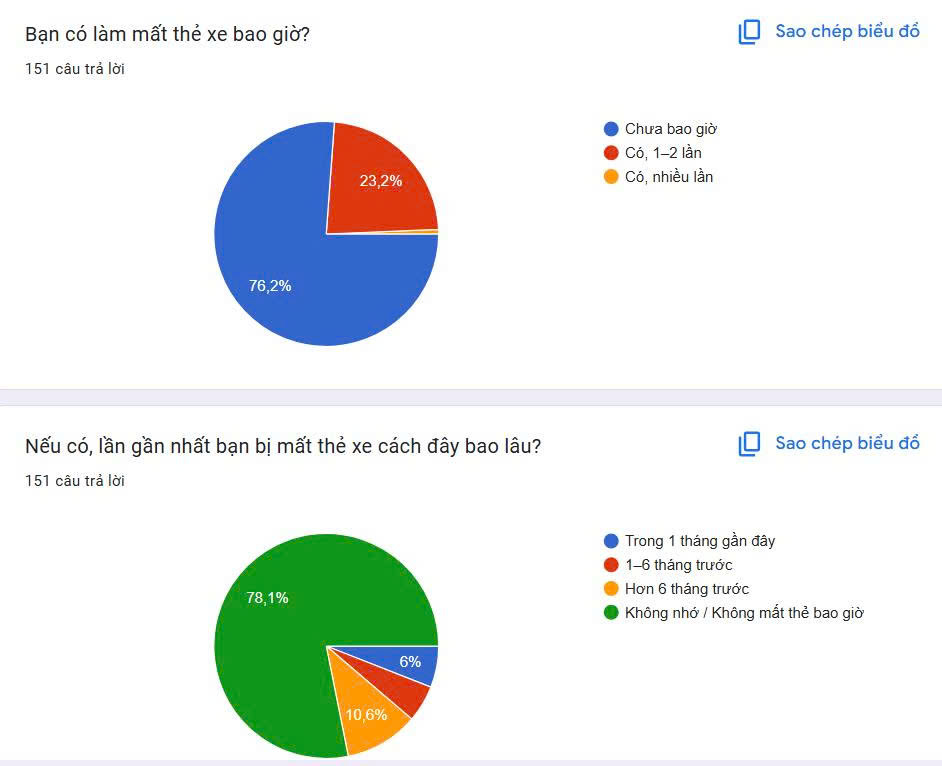
\includegraphics[width=0.9\textwidth]{figures/mat_the.jpg}
    \caption{Kết quả khảo sát về tình trạng mất thẻ xe}
    \label{fig:khaosat1}
\end{figure}

Kết quả cho thấy 76,2\% người tham gia chưa từng bị mất thẻ xe, trong khi 23,2\% đã có trải nghiệm mất thẻ từ 1-2 lần. Đặc biệt, trong số những người từng bị mất thẻ, 78,1\% không nhớ hoặc không có thẻ bảo giờ, điều này cho thấy sự bất tiện lớn của hệ thống thẻ từ truyền thống.

\begin{figure}[H]
    \centering
    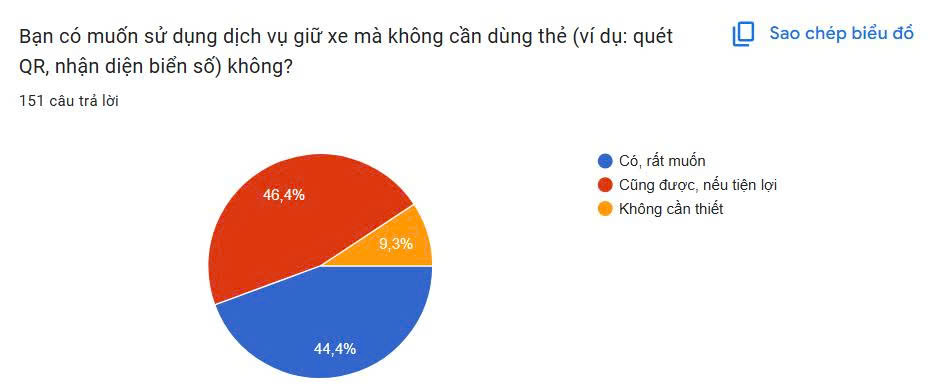
\includegraphics[width=0.9\textwidth]{figures/doi_dv.jpg}
    \caption{Kết quả khảo sát về nhu cầu sử dụng dịch vụ không cần thẻ}
    \label{fig:khaosat2}
\end{figure}
Về nhu cầu sử dụng công nghệ hiện đại, 44,4\% người được hỏi cho biết muốn sử dụng dịch vụ giữ xe không cần thẻ truyền thống , 46,4\% cũng đồng ý nếu tiện lợi hơn và chỉ 9,3\% cho rằng không cần thiết. Điều này chứng tỏ có nhu cầu thực tế cao (90,7\%) đối với giải pháp quản lý bãi đỗ xe thông minh.


Bên cạnh đó, sự phát triển mạnh mẽ của trí tuệ nhân tạo đã mở ra nhiều hướng tiếp cận mới trong việc xây dựng các hệ thống quản lý thông minh. Việc ứng dụng các công nghệ này vào quản lý bãi đỗ xe không chỉ giúp tự động hóa quy trình vận hành mà còn nâng cao hiệu quả quản lý, giảm chi phí nhân lực và cải thiện trải nghiệm người sử dụng.

Xuất phát từ những vấn đề thực tiễn và kết quả khảo sát nêu trên, đề tài Xây dựng hệ thống quản lý bãi đỗ xe thông minh được lựa chọn nhằm nghiên cứu và xây dựng một giải pháp ứng dụng công nghệ hiện đại vào công tác quản lý bãi đỗ xe, loại bỏ sự phụ thuộc vào thẻ từ vật lý, góp phần nâng cao hiệu quả khai thác và vận hành hệ thống.

\section*{2. Tình hình nghiên cứu}
Trong những năm gần đây, nhiều hệ thống quản lý bãi đỗ xe thông minh đã được triển khai sử dụng thẻ từ, mã QR, camera nhận diện biển số và cảm biến phát hiện chỗ trống.

Tại Việt Nam, phần lớn bãi đỗ xe vẫn dùng thẻ từ truyền thống. Theo khảo sát của em thực hiện với 151 người dùng, 23,2\% đã từng mất thẻ xe, trong đó 78,1\% không nhớ hoặc không còn thẻ khi cần lấy xe. Điều này cho thấy hệ thống thẻ từ còn nhiều bất cập.

Một số giải pháp công nghệ cao đã được áp dụng như mã QR hoặc camera nhận diện biển số, nhưng vẫn còn hạn chế về chi phí, khả năng mở rộng và chưa tận dụng triệt để trí tuệ nhân tạo, học sâu cùng điện toán đám mây.

Khảo sát cho thấy 90,7\% người dùng có nhu cầu sử dụng dịch vụ giữ xe không cần thẻ vật lý, chứng tỏ thị trường có tiềm năng lớn cho giải pháp quản lý bãi đỗ xe thông minh.

Do đó, việc xây dựng hệ thống quản lý bãi đỗ xe thông minh sử dụng công nghệ nhận diện biển số và khuôn mặt với chi phí hợp lý là cần thiết và có ý nghĩa thực tiễn tại Việt Nam.
\section*{4. Nhiệm vụ nghiên cứu}
Để đạt được mục tiêu đề ra, đề tài tập trung thực hiện các nhiệm vụ sau:
\begin{itemize}
    \item Khảo sát và phân tích thực trạng quản lý bãi đỗ xe hiện nay.
    \item Nghiên cứu các công nghệ và giải pháp liên quan đến hệ thống quản lý bãi đỗ xe thông minh.
    \item Phân tích yêu cầu chức năng và phi chức năng của hệ thống.
    \item Thiết kế kiến trúc tổng thể, cơ sở dữ liệu và giao diện hệ thống.
    \item Xây dựng và cài đặt hệ thống quản lý bãi đỗ xe thông minh.
    \item Thực hiện kiểm thử và đánh giá kết quả đạt được của hệ thống.
\end{itemize}

\section*{5. Phương pháp nghiên cứu}
Trong quá trình thực hiện đề tài, các phương pháp nghiên cứu sau được sử dụng:
\begin{itemize}
    \item Phương pháp nghiên cứu tài liệu: Thu thập, phân tích các tài liệu, bài báo khoa học và các hệ thống liên quan đến quản lý bãi đỗ xe.
    \item Phương pháp phân tích và thiết kế hệ thống: Phân tích yêu cầu, xây dựng mô hình hệ thống và các sơ đồ UML.
    \item Phương pháp thực nghiệm: Triển khai cài đặt hệ thống, kiểm thử các chức năng và đánh giá hiệu quả hoạt động.
\end{itemize}

\section*{5. Các kết quả đạt được}
Kết quả của đề tài là xây dựng được một hệ thống quản lý bãi đỗ xe thông minh đáp ứng các yêu cầu đề ra. Hệ thống cho phép quản lý xe ra vào một cách tự động, lưu trữ và xử lý dữ liệu chính xác, hỗ trợ giám sát, thống kê và báo cáo tình trạng bãi đỗ xe.

Ngoài ra, đề tài giúp em củng cố và vận dụng kiến thức đã học về lập trình và phân tích thiết kế hệ thống vào thực tế, đồng thời nâng cao kỹ năng nghiên cứu, triển khai và làm việc với các công nghệ mới.
\section*{6. Kết cấu của TTTN}
Bố cục của TTTN được tổ chức thành 5 chương như sau:
\begin{itemize}
    \item \textbf{Chương 1: Cơ sở lý thuyết} - Trình bày các khái niệm, công nghệ và phương pháp liên quan đến hệ thống quản lý bãi đỗ xe thông minh.
    \item \textbf{Chương 2: Phân tích và thiết kế và xây dựng hệ thống} - Phân tích yêu cầu, thiết kế kiến trúc hệ thống và giao diện người dùng.
    \item \textbf{Chương 3: Cài đặt và kiểm thử} - Mô tả quá trình cài đặt, cấu hình và triển khai hệ thống quản lý bãi đỗ xe thông minh.
    \item \textbf{Chương 4: Kết luận và hướng phát triển} - Tổng kết kết quả đạt được, đánh giá hiệu quả của hệ thống và đề xuất hướng phát triển trong tương lai.
\end{itemize}
% Nội dung lời mở đầu...

% 11. CHƯƠNG 1
\chapter{CƠ SỞ LÝ THUYẾT}

\section{Tổng quan bài toán phát hiện hành vi nguy hiểm}

\subsection{Định nghĩa và phạm vi bài toán}

Phát hiện hành vi nguy hiểm từ camera giám sát là bài toán thuộc lĩnh vực thị giác máy tính, nhằm tự động nhận dạng các tình huống đe dọa đến sức khỏe hoặc tính mạng con người thông qua phân tích luồng video theo thời gian thực. Trong phạm vi đề tài này, hành vi nguy hiểm được tập trung vào sự kiện té ngã — một trong những nguyên nhân hàng đầu gây thương tích nghiêm trọng ở người cao tuổi và bệnh nhân.

Bài toán được định nghĩa chính thức như sau: cho một chuỗi khung hình video $\{f_1, f_2, \ldots, f_T\}$ từ camera giám sát, hệ thống cần xác định tại mỗi thời điểm $t$ liệu người trong khung hình có đang thực hiện hành vi té ngã hay không, đồng thời phát cảnh báo tức thời khi phát hiện sự kiện.

\subsection{Các hướng tiếp cận hiện có}

Các phương pháp phát hiện té ngã hiện nay có thể phân thành ba nhóm chính:

\begin{itemize}
    \item \textbf{Dựa trên cảm biến (Sensor-based):} Sử dụng gia tốc kế, con quay hồi chuyển hoặc thiết bị đeo tay để đo chuyển động cơ thể. Ưu điểm là độ chính xác cao trong môi trường kiểm soát, nhưng nhược điểm là yêu cầu người dùng phải luôn mang thiết bị.

    \item \textbf{Dựa trên thị giác máy tính (Vision-based):} Phân tích hình ảnh từ camera mà không cần tiếp xúc trực tiếp. Hướng tiếp cận này đang được nghiên cứu rộng rãi nhờ sự phát triển của các kỹ thuật học sâu.

    \item \textbf{Kết hợp đa phương thức (Multimodal):} Tích hợp nhiều nguồn dữ liệu như camera, cảm biến âm thanh và cảm biến môi trường để tăng độ tin cậy.
\end{itemize}

Đề tài này tập trung vào hướng tiếp cận vision-based, kết hợp ước lượng tư thế người, phân tích luật và mô hình học sâu để đạt được sự cân bằng giữa độ chính xác và tốc độ xử lý thời gian thực.

\subsection{Thách thức và hướng giải quyết}

Bài toán phát hiện té ngã từ camera đối mặt với nhiều thách thức:

\begin{itemize}
    \item \textbf{Phân biệt té ngã với hành động tương tự:} Các hành động như ngồi xuống nhanh hoặc cúi người dễ bị nhầm lẫn với té ngã. Hệ thống kết hợp MediaPipe và YOLOv8-Pose để trích xuất keypoints cơ thể, tính vận tốc và góc nghiêng cơ thể theo thời gian thực. Mô hình Transformer được sử dụng để phân tích chuỗi chuyển động theo thời gian nhằm phân biệt quá trình té ngã với các hoạt động bình thường.


    \item \textbf{Biến đổi góc nhìn và chiếu sáng:} Camera đặt ở các góc độ khác nhau ảnh hưởng đến chất lượng ước lượng tư thế. Giải pháp là fusion hai mô hình MediaPipe và YOLOv8 để bù trừ lỗi.

    \item \textbf{Yêu cầu thời gian thực:} Hệ thống phải phản hồi trong vài giây để cảnh báo kịp thời. Giải pháp là tối ưu pipeline trên GPU và giảm độ trễ WebSocket.

    
\end{itemize}

% ─────────────────────────────────────────────────────────────────────────────

\section{Ước lượng tư thế người}

Ước lượng tư thế người (Human Pose Estimation) là kỹ thuật xác định vị trí các điểm khớp (keypoints) trên cơ thể người trong ảnh hoặc video, bao gồm vai, hông, gối, cổ tay và các khớp khác. Đây là nền tảng để phân tích chuyển động và nhận dạng hành vi.

\subsection{MediaPipe Pose}

MediaPipe Pose là framework ước lượng tư thế người được phát triển bởi Google, hoạt động theo thời gian thực với 33 điểm keypoint trên toàn thân. Framework sử dụng kiến trúc BlazePose — một mạng nơ-ron nhẹ được tối ưu cho thiết bị di động và máy tính cá nhân.

Quá trình xử lý của MediaPipe Pose gồm hai giai đoạn:

\begin{itemize}
    \item \textbf{Giai đoạn phát hiện (Detection):} Một mạng detector nhẹ xác định vùng chứa người trong khung hình.
    \item \textbf{Giai đoạn ước lượng (Estimation):} Mạng chính dự đoán tọa độ $(x, y, z)$ và độ tin cậy (visibility) của 33 keypoint.
\end{itemize}

Mỗi keypoint được biểu diễn bởi vector 4 chiều $(x, y, z, v)$ trong đó $x, y$ là tọa độ pixel đã chuẩn hóa, $z$ là độ sâu tương đối và $v \in [0, 1]$ là độ tin cậy. Trong đề tài này, MediaPipe được sử dụng như mô hình chính để trích xuất tư thế do khả năng xử lý nhanh và ổn định trên CPU.

\subsection{YOLOv8 Pose và ByteTrack}

YOLOv8 Pose là phiên bản mở rộng của kiến trúc YOLO (You Only Look Once) kết hợp phát hiện đối tượng và ước lượng tư thế trong một mô hình duy nhất. Mô hình dự đoán đồng thời bounding box của người và 17 keypoint theo chuẩn COCO.

Kiến trúc YOLOv8 gồm ba thành phần chính:
\begin{itemize}
    \item \textbf{Backbone:} Mạng trích xuất đặc trưng dựa trên CSPNet cải tiến.
    \item \textbf{Neck:} Mạng PAN-FPN tổng hợp đặc trưng đa tỉ lệ.
    \item \textbf{Head:} Đầu ra song song cho bounding box và keypoints.
\end{itemize}

ByteTrack là thuật toán theo dõi đa đối tượng (Multi-Object Tracking) được tích hợp vào YOLOv8 để duy trì ID ổn định cho mỗi người qua các khung hình. Thuật toán sử dụng IoU (Intersection over Union) kết hợp với bộ lọc Kalman để dự đoán vị trí và liên kết detection giữa các frame liên tiếp.

\subsection{Fusion đa mô hình}

Để tận dụng ưu điểm của cả hai mô hình, hệ thống thực hiện fusion có trọng số theo độ tin cậy:

\begin{equation}
    m_{fused} = \frac{w_{mp} \cdot m_{mp} + w_{yolo} \cdot m_{yolo}}{w_{mp} + w_{yolo}}
\end{equation}

trong đó $w_{mp}$ và $w_{yolo}$ lần lượt là độ tin cậy của MediaPipe và YOLOv8, $m$ là các chỉ số tư thế cần fusion (góc cơ thể, tỉ lệ bounding box). Vector đặc trưng thô được ghép nối từ 33 keypoint MediaPipe và 17 keypoint YOLO tạo thành vector 200 chiều đầu vào cho mô hình Transformer.

% ─────────────────────────────────────────────────────────────────────────────

\section{Phát hiện té ngã}

\subsection{Phương pháp dựa trên luật}

Phương pháp rule-based phát hiện té ngã dựa trên việc phân tích các đặc trưng hình học và vận tốc của cơ thể người theo thời gian. Phương pháp này có ưu điểm là có thể giải thích được (explainable) và không yêu cầu dữ liệu huấn luyện.

\subsection{Phân loại tư thế và phân tích vận tốc}

Hệ thống phân loại tư thế người thành bốn trạng thái: STANDING (đứng), SITTING (ngồi), LYING (nằm) và WALKING (đi lại). Việc phân loại dựa trên hai chỉ số chính:

\begin{itemize}
    \item \textbf{Góc cơ thể (body\_angle):} Góc giữa vector cột sống (từ vai đến hông) và trục thẳng đứng, tính theo công thức:
    \begin{equation}
        \theta = \arctan\left(\frac{|\Delta x_{spine}|}{|\Delta y_{spine}| + \epsilon}\right)
    \end{equation}
    Khi $\theta \geq 75°$, người được phân loại là LYING.

    \item \textbf{Tỉ lệ bounding box (aspect\_ratio):} Tỉ lệ chiều cao trên chiều rộng của bounding box $r = h/w$. Khi $r \leq 0.45$, người được phân loại là LYING.
\end{itemize}

Vận tốc hướng xuống của trọng tâm cơ thể được tính theo cửa sổ trượt:
\begin{equation}
    v_y = \frac{y_{center}(t) - y_{center}(t - \Delta t)}{\Delta t}
\end{equation}

Sự kiện té ngã được xác nhận khi thỏa mãn đồng thời các điều kiện: vận tốc đủ lớn ($v_y > v_{threshold}$), có lịch sử tư thế đứng/ngồi/đi, trạng thái LYING duy trì đủ số frame, thời gian chuyển trạng thái đủ ngắn, và không phải hành động cúi người.

\subsection{Mạng Transformer cho nhận dạng hành động}

Kiến trúc Transformer, được giới thiệu bởi Vaswani et al. (2017) trong bài báo ``Attention is All You Need'', ban đầu được thiết kế cho xử lý ngôn ngữ tự nhiên nhưng đã chứng minh hiệu quả vượt trội trong nhận dạng hành động từ chuỗi tư thế. Ưu điểm của Transformer so với RNN/LSTM là khả năng học mối quan hệ dài hạn giữa các frame thông qua cơ chế Self-Attention mà không bị giới hạn bởi độ dài chuỗi.

\textbf{Cơ chế Self-Attention} cho phép mô hình học được mối quan hệ giữa các frame trong chuỗi thời gian. Cho chuỗi đầu vào $X \in \mathbb{R}^{T \times d}$, Self-Attention được tính:

\begin{equation}
    \text{Attention}(Q, K, V) = \text{softmax}\left(\frac{QK^T}{\sqrt{d_k}}\right)V
\end{equation}

trong đó $Q = XW^Q$, $K = XW^K$, $V = XW^V$ là các ma trận Query, Key, Value; $d_k$ là chiều của không gian key. Multi-Head Attention kết hợp $h$ đầu attention song song để học nhiều mối quan hệ khác nhau:

\begin{equation}
    \text{MultiHead}(Q,K,V) = \text{Concat}(\text{head}_1, \ldots, \text{head}_h)W^O
\end{equation}

\textbf{Positional Embedding} là tham số học được $P \in \mathbb{R}^{(T+1) \times d_{model}}$ được cộng vào biểu diễn đầu vào để đưa thông tin vị trí thời gian vào mô hình, do Transformer không có tính chất tuần tự như RNN.

\textbf{CLS Token} là một vector đặc biệt $\mathbf{c} \in \mathbb{R}^{d_{model}}$ được thêm vào đầu chuỗi, học cách tổng hợp thông tin toàn chuỗi để phục vụ phân loại:

\begin{equation}
    \hat{y} = \text{MLP}(\text{TransformerEncoder}([\mathbf{c}; x_1; \ldots; x_T])[0])
\end{equation}

\subsection{Kết hợp Rule-based và AI}

Hệ thống sử dụng chiến lược AND logic — cả hai thành phần phải đồng ý mới phát cảnh báo:

\begin{equation}
    \text{fall\_detected} = \text{rule\_fall} \wedge \text{ai\_fall}
\end{equation}

Trong đó $\text{rule\_fall}$ là kết quả từ FallDetector (rule-based) và $\text{ai\_fall}$ là kết quả từ TransformerEngine với ngưỡng xác suất $p_{fall} \geq 0.65$. Chiến lược này giúp giảm cả false positive lẫn false negative so với dùng từng phương pháp riêng lẻ.

\subsection{Đánh giá mô hình với K-Fold Cross Validation}

K-Fold Cross Validation là kỹ thuật đánh giá mô hình học máy nhằm giảm thiểu sự phụ thuộc vào cách phân chia tập dữ liệu, đặc biệt hữu ích khi dữ liệu có kích thước giới hạn.

Quy trình K-Fold Cross Validation gồm các bước sau:

\begin{enumerate}
    \item Chia toàn bộ dataset $\mathcal{D}$ thành $K$ phần (fold) có kích thước xấp xỉ bằng nhau: $\mathcal{D} = \{D_1, D_2, \ldots, D_K\}$.
    \item Lặp $K$ lần: ở vòng lặp thứ $i$, sử dụng $D_i$ làm tập validation và $K-1$ phần còn lại làm tập huấn luyện.
    \item Huấn luyện và đánh giá mô hình tại mỗi fold, thu được độ chính xác $\text{acc}_i$.
    \item Tính độ chính xác trung bình và độ lệch chuẩn:
    \begin{equation}
        \overline{\text{acc}} = \frac{1}{K}\sum_{i=1}^{K}\text{acc}_i, \qquad
        \sigma = \sqrt{\frac{1}{K}\sum_{i=1}^{K}(\text{acc}_i - \overline{\text{acc}})^2}
    \end{equation}
\end{enumerate}

Ưu điểm của K-Fold so với phân chia train/test đơn giản:

\begin{itemize}
    \item \textbf{Đánh giá tin cậy hơn:} Mỗi mẫu dữ liệu được dùng làm validation đúng một lần, tránh sự ngẫu nhiên của một lần phân chia.
    \item \textbf{Phát hiện overfitting:} Độ lệch chuẩn $\sigma$ cao giữa các fold cho thấy mô hình không ổn định và có thể đang overfit trên một phần dữ liệu.
    \item \textbf{Tận dụng toàn bộ dữ liệu:} Đặc biệt quan trọng khi tập dữ liệu nhỏ, vì tất cả các mẫu đều được dùng cho cả huấn luyện lẫn đánh giá.
\end{itemize}

Đề tài sử dụng Stratified K-Fold với $K = 5$, đảm bảo tỉ lệ nhãn \textit{fall}/\textit{non\_fall} được giữ nguyên trong mỗi fold để tránh mất cân bằng dữ liệu ảnh hưởng đến kết quả đánh giá. Ngoài ra, kỹ thuật data augmentation (lật ngang, thay đổi tốc độ, thêm nhiễu Gaussian) chỉ được áp dụng trên tập huấn luyện của từng fold, không áp dụng trên tập validation, đảm bảo đánh giá khách quan.

% ─────────────────────────────────────────────────────────────────────────────

\section{Nhận diện khuôn mặt}

\subsection{RetinaFace và ArcFace}

RetinaFace là mô hình phát hiện khuôn mặt (face detection) đa tác vụ, đồng thời dự đoán bounding box khuôn mặt, 5 điểm landmark (mắt, mũi, miệng) và điểm tin cậy. Mô hình sử dụng kiến trúc Feature Pyramid Network để phát hiện khuôn mặt ở nhiều tỉ lệ khác nhau, phù hợp với môi trường camera giám sát có nhiều người ở các khoảng cách khác nhau.

ArcFace (Additive Angular Margin Loss) là phương pháp học biểu diễn khuôn mặt (face representation) hiện đại, huấn luyện mạng để tạo ra vector đặc trưng 512 chiều cho mỗi khuôn mặt. ArcFace thêm margin góc $m$ vào hàm loss để tăng khả năng phân biệt giữa các danh tính:

\begin{equation}
    \mathcal{L} = -\frac{1}{N}\sum_{i=1}^{N}\log\frac{e^{s\cos(\theta_{y_i} + m)}}{e^{s\cos(\theta_{y_i}+m)} + \sum_{j \neq y_i} e^{s\cos\theta_j}}
\end{equation}

trong đó $\theta_{y_i}$ là góc giữa vector đặc trưng và trọng số lớp, $s$ là hệ số tỉ lệ và $m$ là margin góc.

\subsection{Cosine Similarity}

Để so sánh hai vector đặc trưng khuôn mặt $\mathbf{u}$ và $\mathbf{v}$, hệ thống sử dụng độ tương đồng cosine:

\begin{equation}
    \text{sim}(\mathbf{u}, \mathbf{v}) = \frac{\mathbf{u} \cdot \mathbf{v}}{\|\mathbf{u}\| \cdot \|\mathbf{v}\|}
\end{equation}

Giá trị $\text{sim} \in [-1, 1]$, trong đó giá trị càng gần 1 thì hai khuôn mặt càng giống nhau. Ngưỡng nhận dạng được đặt tại $\text{sim} \geq 0.6$ để cân bằng giữa false accept rate và false reject rate.

% ─────────────────────────────────────────────────────────────────────────────

% ─────────────────────────────────────────────────────────────────────────────

\section{Các công nghệ sử dụng}

\subsection{FastAPI}

FastAPI là framework Python hiện đại để xây dựng REST API, dựa trên tiêu chuẩn OpenAPI và JSON Schema. FastAPI sử dụng type hints của Python và Pydantic để tự động xác thực dữ liệu đầu vào, đồng thời tự động sinh tài liệu API tương tác (Swagger UI). Framework hỗ trợ lập trình bất đồng bộ (async/await) với ASGI, cho phép xử lý hàng nghìn kết nối đồng thời với hiệu năng cao.

\subsection{Flutter}

Flutter là framework phát triển ứng dụng đa nền tảng của Google, sử dụng ngôn ngữ Dart. Flutter biên dịch trực tiếp sang mã máy native, cho hiệu năng gần tương đương ứng dụng native. Hệ thống widget phong phú cho phép xây dựng giao diện đẹp, nhất quán trên cả Android và iOS từ một codebase duy nhất. Ứng dụng mobile trong đề tài sử dụng Provider cho quản lý trạng thái và GoRouter cho điều hướng.

\subsection{NuxtJS}

NuxtJS là framework Vue.js cho phát triển ứng dụng web, hỗ trợ Server-Side Rendering (SSR) và Static Site Generation (SSG). Trong đề tài, NuxtJS được dùng để xây dựng giao diện web quản trị cho phép admin theo dõi và quản lý hệ thống từ trình duyệt.

\subsection{PostgreSQL và Neon}

PostgreSQL là hệ quản trị cơ sở dữ liệu quan hệ mã nguồn mở, nổi tiếng với tính ổn định, hỗ trợ ACID và khả năng mở rộng. Neon là dịch vụ PostgreSQL serverless trên đám mây, cho phép tự động mở rộng theo tải và tách biệt môi trường đọc/ghi để tối ưu hiệu năng. Hệ thống sử dụng SQLAlchemy với chế độ async (asyncpg) để truy vấn không đồng bộ.

\subsection{Firebase Authentication}

Firebase Authentication là dịch vụ xác thực của Google, cung cấp cơ chế đăng nhập an toàn với nhiều phương thức như email/mật khẩu và OAuth. Hệ thống sử dụng JWT (JSON Web Token) từ Firebase để xác thực người dùng tại backend, đảm bảo mỗi request đều được kiểm tra quyền truy cập.

\subsection{Cloudinary}

Cloudinary là dịch vụ lưu trữ và quản lý media trên đám mây, hỗ trợ upload, chuyển đổi và phân phối ảnh/video qua CDN toàn cầu. Khi phát hiện té ngã, hệ thống cắt đoạn video 6 giây (90 frame trước + 90 frame sau sự kiện) và upload lên Cloudinary để lưu trữ và chia sẻ qua URL với người thân.

% \subsection{ONNX Runtime}

% ONNX (Open Neural Network Exchange) là định dạng chuẩn mở để lưu trữ và triển khai mô hình học máy. ONNX Runtime là engine tối ưu hóa thực thi mô hình ONNX, hỗ trợ tăng tốc trên nhiều loại phần cứng (CPU, GPU, NPU). Trong hệ thống, ONNX Runtime được sử dụng để triển khai mô hình nhận diện khuôn mặt (RetinaFace/ArcFace) với hiệu năng cao mà không cần framework học sâu đầy đủ.

% 12. CHƯƠNG 2
% \chapter{PHÂN TÍCH, THIẾT KẾ VÀ XÂY DỰNG HỆ THỐNG}

% \section{Yêu cầu chức năng}
% \section{Yêu cầu phi chức năng}
% \section{Kiến trúc hệ thống}
% \section{Sơ đồ Use Case}
% \section{Sơ đồ lớp}
% \section{Sơ đồ activity}
% \section{Thiết kế cơ sở dữ liệu}
% \section{Thiết kế giao diện}


\chapter{PHÂN TÍCH, THIẾT KẾ VÀ XÂY DỰNG HỆ THỐNG}

\section{Yêu cầu chức năng}

Dựa trên phân tích nghiệp vụ và khảo sát thực tế, hệ thống quản lý bãi đỗ xe thông minh cần đáp ứng các yêu cầu chức năng sau đây.

\begin{figure}[H]
    \centering
    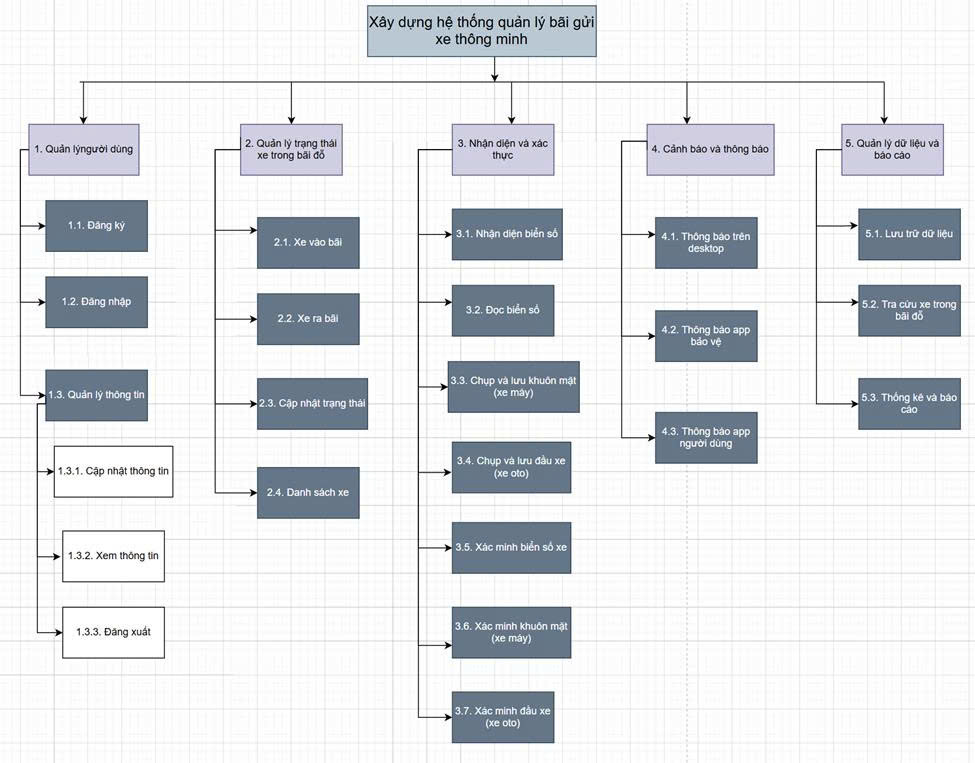
\includegraphics[width=1.0\textwidth]{figures/fdd.jpg}
    \caption{Sơ đồ phân tách chức năng hệ thống (FDD)}
    \label{fig:fdd}
\end{figure}

Hệ thống được phân tách thành 5 nhóm chức năng chính như Hình \ref{fig:fdd}: (1) Quản lý người dùng, (2) Quản lý trạng thái xe trong bãi đỗ, (3) Nhận diện và xác thực, (4) Cảnh báo và thông báo, (5) Quản lý dữ liệu và báo cáo. Các chức năng này được triển khai trên ba thành phần chính của hệ thống: Desktop Application, Mobile Application cho người dùng, và Mobile Application cho bảo vệ. Dưới đây là mô tả chi tiết yêu cầu chức năng theo từng thành phần ứng dụng.
\subsection{Yêu cầu chức năng cho Desktop Application}

\begin{itemize}
    \item Nhận diện biển số xe:
    \begin{itemize}
        \item Tự động phát hiện và đọc biển số xe khi xe vào/ra bãi đỗ
        \item Hỗ trợ nhận diện biển số xe Việt Nam các loại
        \item Lưu trữ ảnh biển số và thông tin nhận diện
        \item Độ chính xác tối thiểu 95\%
    \end{itemize}
    
    \item Nhận diện khuôn mặt cho xe máy:
    \begin{itemize}
        \item Phát hiện và trích xuất đặc trưng khuôn mặt người lái xe
        \item Chụp và lưu trữ ảnh khuôn mặt khi xe vào bãi
        \item So khớp với cơ sở dữ liệu khuôn mặt đã đăng ký
        \item Xác thực danh tính khi xe vào và ra khỏi bãi
        \item Cảnh báo khi phát hiện khuôn mặt không khớp
    \end{itemize}
    
    \item Xác minh xe máy khi ra bãi:
    \begin{itemize}
        \item So sánh khuôn mặt người lái khi ra với khuôn mặt khi vào
        \item Tính toán độ tương đồng khuôn mặt (similarity score)
        \item Xác minh biển số xe khớp với thông tin đã lưu
        \item Cảnh báo khi độ tương đồng cao hơn ngưỡng cho phép  
        \item Yêu cầu xác nhận từ chủ xe qua mobile app nếu phát hiện bất thường
    \end{itemize}
    
    \item Nhận diện logo và đặc trưng xe ô tô:
    \begin{itemize}
        \item Phát hiện và nhận dạng logo thương hiệu xe ô tô
        \item Chụp và lưu trữ ảnh crop và toàn cảnh xe khi vào  bãi
        \item Trích xuất đặc trưng đầu xe bằng Siamese Network
        \item Lưu trữ vào database
    \end{itemize}
    
    \item Xác minh xe ô tô khi ra bãi:
    \begin{itemize}
        \item Chụp ảnh xe hiện tại và trích xuất đặc trưng
        \item So sánh đặc trưng xe ra với đặc trưng xe vào bằng Siamese Network
        \item Tính toán độ tương đồng giữa hai ảnh xe 
        \item So sánh logo xe vào và xe ra
        \item Xác minh biển số xe khớp với thông tin đã lưu
        \item Cảnh báo khi độ tương đồng cao hơn ngưỡng cho phép 
        \item Yêu cầu xác nhận từ chủ xe qua mobile app nếu phát hiện bất thường
    \end{itemize}
    
    \item Quản lý cảnh báo:
    \begin{itemize}
        \item Phát hiện xe ra không có xác nhận từ mobile app
        \item Phát hiện khuôn mặt/xe không khớp với dữ liệu vào
        \item Tạo và gửi cảnh báo đến ứng dụng bảo vệ
        \item Hiển thị thông tin chi tiết về cảnh báo (ảnh so sánh, độ tương đồng)
        \item Chặn xe khi phát hiện bất thường nghiêm trọng
    \end{itemize}
    
    \item Giao diện giám sát:
    \begin{itemize}
        \item Hiển thị luồng video từ camera real-time
        \item Hiển thị kết quả nhận diện trên màn hình
        \item Hiển thị kết quả so sánh khi xe ra (khuôn mặt, xe, độ tương đồng)
        \item Log các sự kiện hệ thống
    \end{itemize}
\end{itemize}

\subsection{Yêu cầu chức năng cho Mobile Application (Người dùng)}

\begin{itemize}
    \item Quản lý tài khoản:
    \begin{itemize}
        \item Đăng ký tài khoản mới
        \item Đăng nhập/đăng xuất
        \item Cập nhật thông tin cá nhân
        \item Đổi mật khẩu
    \end{itemize}
    
    \item Quản lý phương tiện:
    \begin{itemize}
        \item Đăng ký biển số xe 
        \item Đăng ký khuôn mặt cho xe máy 
        \item Chỉnh sửa thông tin xe
        \item Xóa xe khỏi hệ thống
    \end{itemize}
    
    \item Xác nhận rời bãi đỗ xe:
    \begin{itemize}
        \item Hiển thị danh sách xe đang đỗ trong bãi
        \item Chọn xe và bấm nút "Xác nhận rời đi"
        \item Hiển thị thông tin thời gian đỗ
    \end{itemize}
    
    \item Xem lịch sử:
    \begin{itemize}
        \item Xem lịch sử các lần vào/ra bãi đỗ
        \item Lọc theo thời gian, xe
        \item Xem chi tiết từng lần đỗ (thời gian vào, ra)
        \item Xuất báo cáo định kỳ
    \end{itemize}
    
    \item Nhận thông báo:
    \begin{itemize}
        \item Thông báo khi xe được xác nhận vào bãi
        \item Thông báo khi có cảnh báo về xe
        \item Nhắc nhở khi xe đỗ quá thời gian cho phép

    \end{itemize}
\end{itemize}

\subsection{Yêu cầu chức năng cho Mobile Application (Bảo vệ)}

\begin{itemize}
    \item Đăng nhập và xác thực:
    \begin{itemize}
        \item Đăng nhập với tài khoản bảo vệ
      
        \item Quản lý phiên làm việc
    \end{itemize}
    
    \item Giám sát xe trong bãi:
    \begin{itemize}
        \item Xem danh sách tất cả xe đang đỗ
        \item Hiển thị thông tin: biển số, loại xe, thời gian vào, vị trí
        \item Tìm kiếm xe theo biển số
        \item Lọc theo loại xe, khu vực
        \item Xem sơ đồ bãi đỗ với vị trí các xe
        \item Cập nhật real-time khi có xe vào/ra
    \end{itemize}
    
    \item Xem lịch sử ra vào:
    \begin{itemize}
        \item Tra cứu lịch sử của từng xe cụ thể
        \item Lọc theo khoảng thời gian
        \item Xem ảnh chụp khi xe vào/ra
        \item Xem video giám sát (nếu có)
        \item Xuất báo cáo chi tiết
        \item Thống kê theo ngày/tuần/tháng
    \end{itemize}
    
    \item Xử lý cảnh báo:
    \begin{itemize}
        \item Nhận thông báo cảnh báo real-time
   
        \item Phê duyệt hoặc từ chối cho xe ra
        \item Cập nhật trạng thái cảnh báo
       
        \item Báo cáo cho bảo vệ
    \end{itemize}
    
    
\end{itemize}

\section{Yêu cầu phi chức năng}

\subsection{Hiệu năng }

\begin{itemize}
    \item Thời gian phản hồi:
    \begin{itemize}
        \item Nhận diện biển số xe: $\leq 10$ giây
        \item Nhận diện khuôn mặt: $\leq 5$ giây
        \item Nhận diện logo: $\leq 2$ giây
        \item So sánh Siamese Network: $\leq 7$ giây
        \item Tải danh sách xe trong bãi: $\leq 3$ giây
    \end{itemize}
    
    \item Độ chính xác AI Models:
    \begin{itemize}
        \item Nhận diện biển số: $\geq 95\%$
        \item Nhận diện khuôn mặt: $\geq 98\%$ (False Acceptance Rate < 0.1\%)
        \item Nhận diện logo xe: $\geq 90\%$
        \item So sánh Siamese : $\geq 95\%$ (threshold similarity < 0.5)
    \end{itemize}
    
    
    
    \item Dung lượng lưu trữ:
    \begin{itemize}
        \item Lưu trữ tối thiểu 100,000 bản ghi lịch sử
        \item Lưu trữ ảnh/video tối đa 30 ngày
        
    \end{itemize}
\end{itemize}


\section{Kiến trúc hệ thống}

\subsection{Tổng quan kiến trúc}

Hệ thống gồm ba thành phần chính: ứng dụng desktop, backend server và ứng dụng mobile. Mỗi thành phần đảm nhiệm một vai trò riêng nhưng phối hợp chặt chẽ thông qua các giao thức và API thống nhất.

\begin{itemize}
    \item Ứng dụng desktop đóng vai trò client chính, thực hiện các tác vụ xử lý trí tuệ nhân tạo và giao tiếp trực tiếp với camera.
    \item Backend server chịu trách nhiệm xử lý nghiệp vụ, quản lý dữ liệu và cung cấp API cho các client.
    \item Ứng dụng mobile cho phép người dùng và nhân viên bảo vệ tương tác, theo dõi trạng thái và nhận thông báo theo thời gian thực.
\end{itemize}

\subsection{Kiến trúc ứng dụng Desktop}

Ứng dụng desktop được phát triển bằng Python, đảm nhiệm các tác vụ xử lý nặng như:
\begin{itemize}
    \item Nhận diện biển số xe bằng mô hình YOLOv8.
    \item Nhận diện khuôn mặt cho bãi xe máy.
    \item Nhận diện logo và so khớp xe ô tô bằng mạng Siamese.
    \item Xử lý luồng video từ camera theo thời gian thực.
\end{itemize}

Sau khi xử lý, kết quả được gửi về backend thông qua FLASK API để lưu trữ và đồng bộ với các client khác.

\subsection{Kiến trúc Backend}

Backend server được xây dựng theo mô hình kiến trúc MVC, trong đó:
\begin{itemize}
    \item Model quản lý dữ liệu và kết nối với các hệ cơ sở dữ liệu.
    \item Controller xử lý logic nghiệp vụ, tiếp nhận và phản hồi các request từ client.
    \item View được thể hiện dưới dạng dữ liệu JSON trả về cho các ứng dụng client.
\end{itemize}


\subsection{Kiến trúc ứng dụng Mobile}

Ứng dụng mobile được phát triển bằng Kotlin theo mô hình MVVM, bao gồm:
\begin{itemize}
    \item View hiển thị giao diện người dùng.
    \item ViewModel xử lý logic hiển thị và quản lý trạng thái.
    \item Model đại diện cho dữ liệu và giao tiếp với backend thông qua API.
\end{itemize}

Kiến trúc MVVM giúp tách biệt rõ ràng giữa giao diện và logic xử lý, tăng khả năng mở rộng và dễ bảo trì.

\subsection{Kiến trúc lưu trữ dữ liệu}

Hệ thống sử dụng nhiều nền tảng lưu trữ phù hợp với từng loại dữ liệu:
\begin{itemize}
    \item Firebase Realtime Database để đồng bộ trạng thái xe và cảnh báo theo thời gian thực.
    \item MongoDB để lưu trữ thông tin người dùng, phương tiện và lịch sử ra vào.
    \item Cloudinary để lưu trữ và quản lý hình ảnh biển số, khuôn mặt và phương tiện.
\end{itemize}

Dưới đây là sơ đồ kiến trúc tổng thể của hệ thống quản lý bãi đỗ xe thông minh:
\begin{figure}[H]
\centering
\begin{tikzpicture}[
    box/.style={draw, rectangle, rounded corners, minimum width=2.5cm, minimum height=0.8cm, align=center, font=\small},
    arrow/.style={->, thick}
]

% Camera
\node[box] (camera) {Camera};

% Desktop
\node[box, below=1.2cm of camera] (desktop) {Desktop App\\AI Processing\\YOLOv8, Deep Learning};

% Backend
\node[box, right=2.5cm of desktop] (backend) {Backend Server\\MVC Architecture};

% Mobile
\node[box, below=1.2cm of backend] (mobile) {Mobile App\\Kotlin -- MVVM};

% Databases - DI CHUYỂN QUA TRÁI
\node[box, right=2.5cm of backend] (db1) {Realtime Database};
\node[box, below=0.8cm of db1] (db2) {MongoDB};
\node[box, below=0.8cm of db2] (cloud) {Cloudinary};

% Arrows
\draw[arrow] (camera) -- (desktop);
\draw[arrow] (desktop) -- node[above, font=\tiny]{FlaskAPI} (backend);
\draw[arrow] (backend) -- (mobile);

\draw[arrow] (backend) -- (db1);
\draw[arrow] (backend) -- (db2);
\draw[arrow] (backend) -- (cloud);

\end{tikzpicture}
\caption{Kiến trúc tổng thể hệ thống quản lý bãi đỗ xe thông minh}
\end{figure}



\section{Sơ đồ Use Case tổng quát}
\begin{figure}[H]
    \centering
    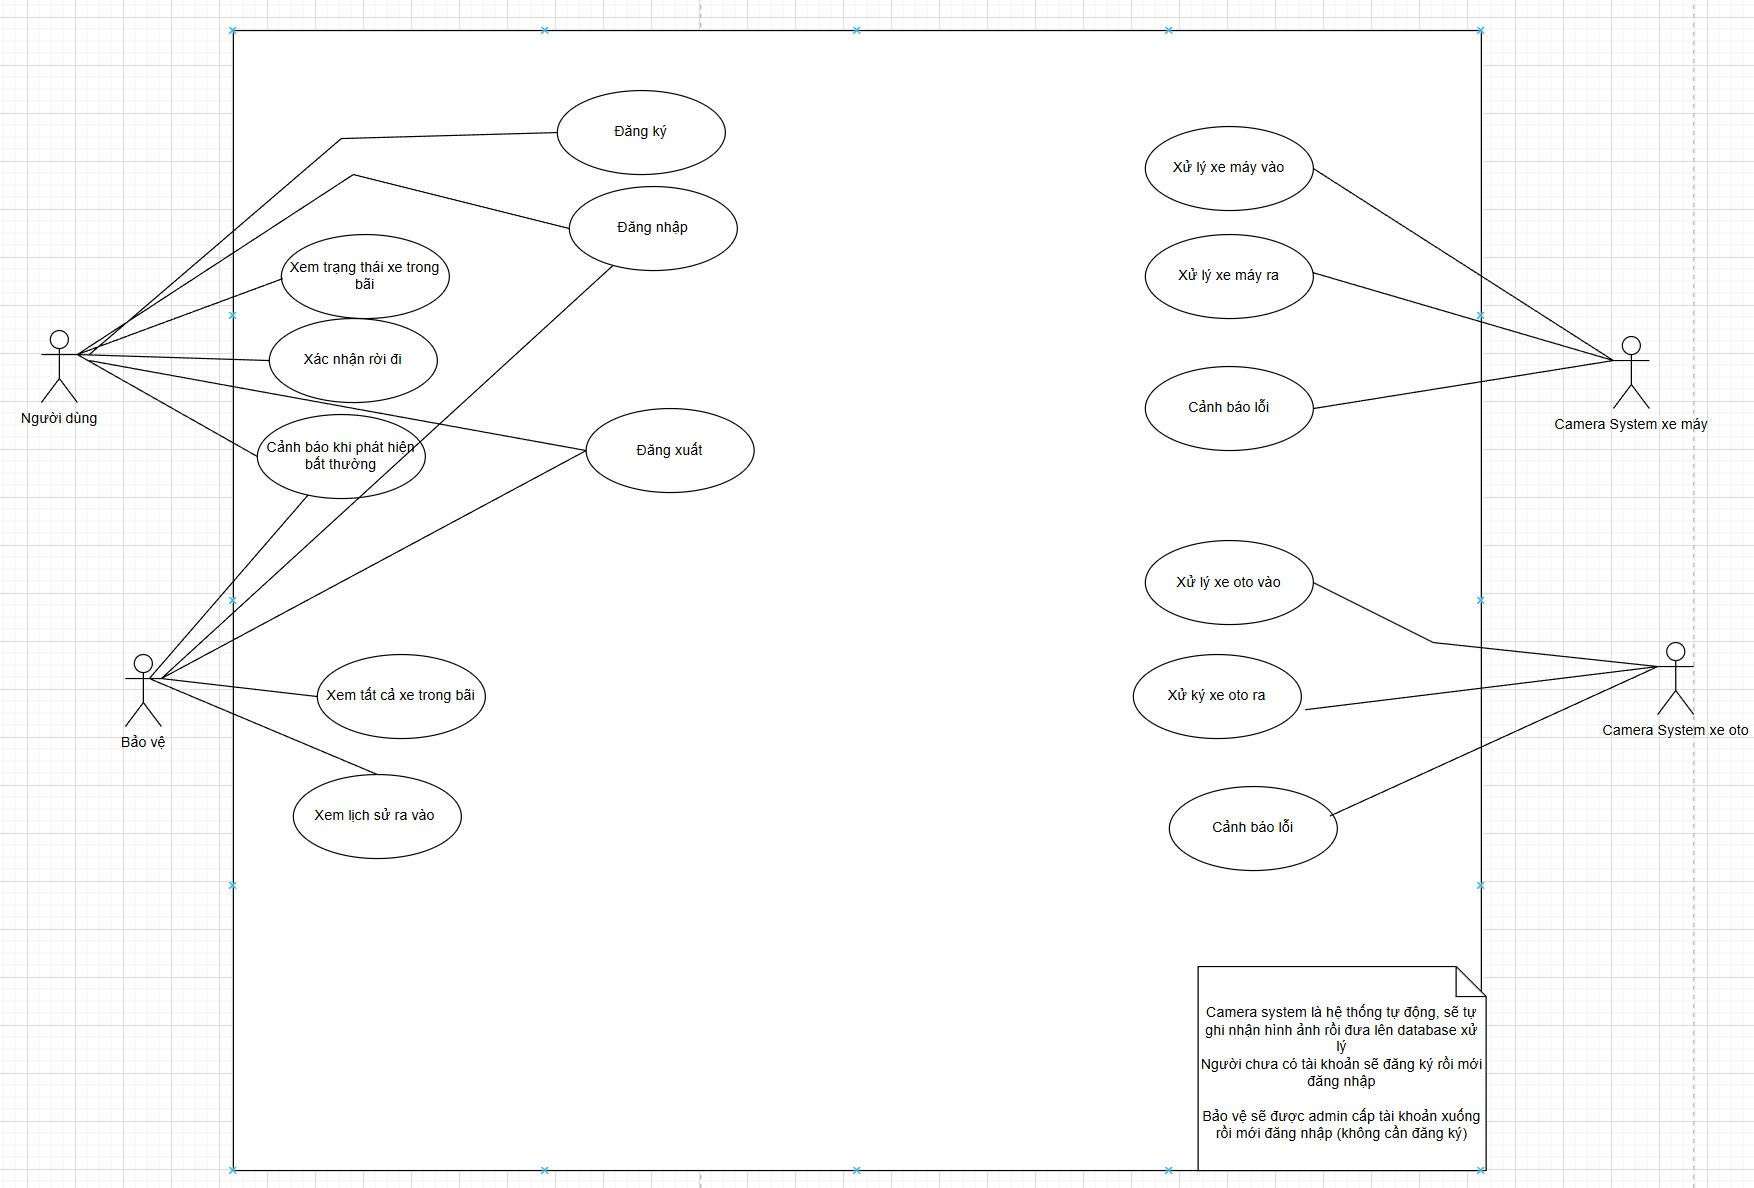
\includegraphics[width=1.0\textwidth]{figures/tq.jpg}
    \caption{Sơ đồ Use Case  tổng quát}
    \label{fig:usecase_tq}
\end{figure}

\subsection{Các actor trong hệ thống}

Hệ thống quản lý bãi đỗ xe thông minh bao gồm 4 actor chính như được thể hiện trong Hình \ref{fig:usecase_tq}:

\begin{itemize}
    \item \textbf{Người dùng (Chủ xe):} Người sở hữu phương tiện và sử dụng dịch vụ bãi đỗ xe. Actor này tương tác với hệ thống thông qua mobile application để đăng ký tài khoản, quản lý thông tin xe, xác nhận rời bãi đỗ, xem lịch sử và nhận thông báo về trạng thái xe.
    
    \item \textbf{Bảo vệ:} Nhân viên bảo vệ quản lý và giám sát bãi đỗ xe. Actor này sử dụng mobile application để xem danh sách xe trong bãi, tra cứu lịch sử ra vào, xử lý các cảnh báo bất thường và phê duyệt xe ra trong trường hợp cần thiết. Bảo vệ được cấp tài khoản riêng với quyền hạn cao hơn người dùng thường.
    
    \item \textbf{Camera System xe máy:} Hệ thống camera tự động tại cổng xe máy, chịu trách nhiệm chụp ảnh, nhận diện biển số xe và khuôn mặt người lái khi xe vào/ra. Hệ thống sẽ so sánh khuôn mặt người lái khi ra với dữ liệu đã lưu khi vào để phát hiện bất thường. Camera system là actor không phải con người, tự động hóa hoàn toàn.
    
    \item \textbf{Camera System xe ô tô:} Hệ thống camera tự động tại cổng xe ô tô, thực hiện chụp ảnh, nhận diện biển số xe, logo thương hiệu và đặc trưng toàn bộ xe sử dụng Siamese Network. Khi xe ra, hệ thống sẽ so sánh hình ảnh xe hiện tại với ảnh đã lưu khi vào để xác minh và phát hiện bất thường.
\end{itemize}

\textit{Lưu ý:} Camera System được xem là một actor trong hệ thống vì có khả năng tương tác chủ động và trực tiếp mà không cần sự can thiệp của con người. Hệ thống camera tự động thu thập dữ liệu (biển số, khuôn mặt, đặc trưng phương tiện), xử lý bằng các mô hình AI như YOLOv8, CNN, DeepFace và Siamese Network, từ đó kích hoạt các use case như nhận diện, xác minh và cảnh báo. Đây là một actor phi con người (non-human actor), hoạt động độc lập và tự động hóa toàn bộ quy trình kiểm soát xe ra vào. Người dùng chỉ cần đăng ký thông tin một lần và xác nhận lấy xe qua ứng dụng di động. Và bảo vệ thực hiện giám sát và xử lý các tình huống bất thường.




\subsection{Sơ đồ Use Case chi tiết cho camera systemxe máy }

\begin{figure}[H]
    \centering
    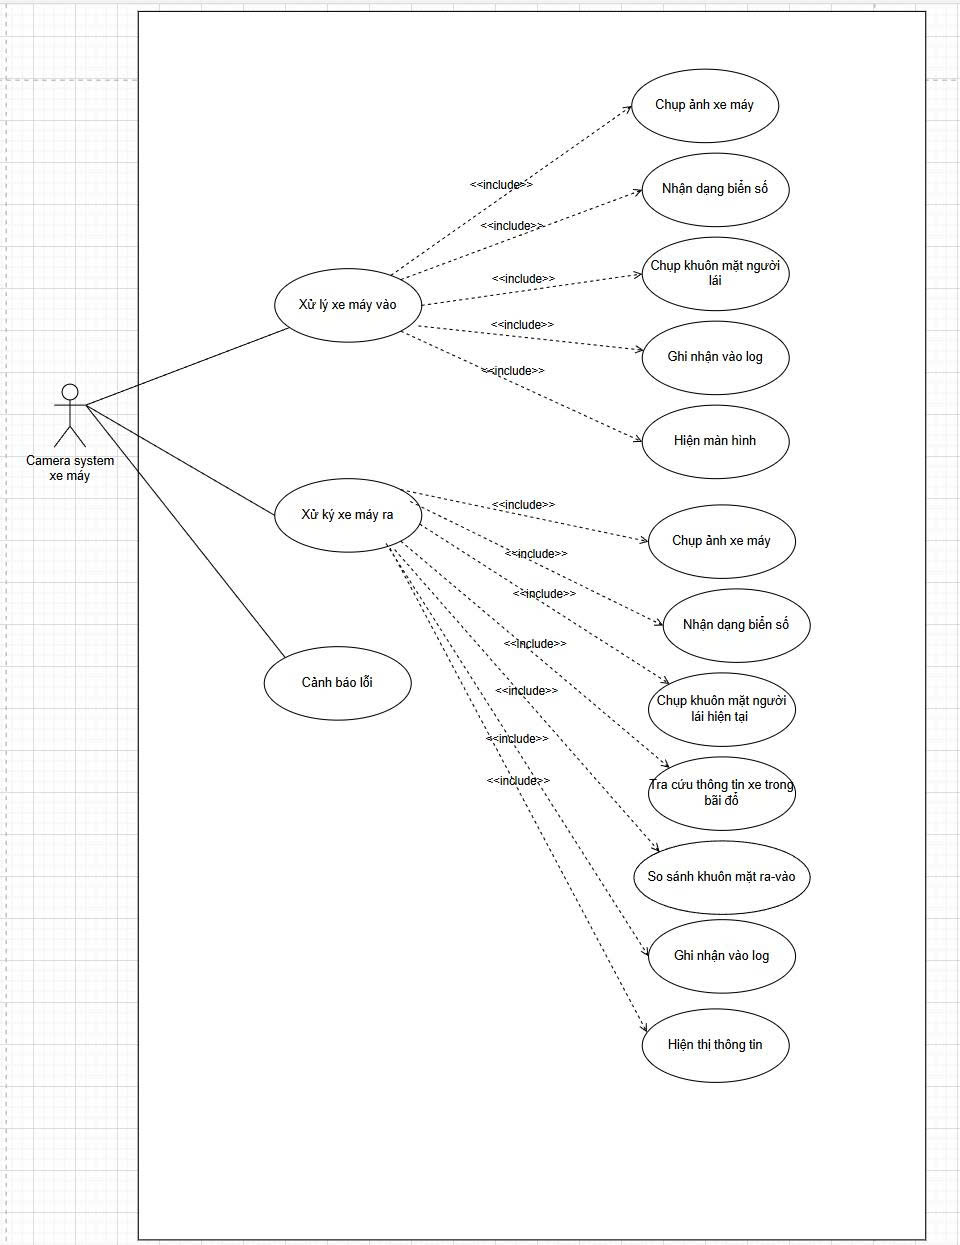
\includegraphics[width=0.85\textwidth]{figures/usecase_xemay.jpg}
    \caption{Sơ đồ Use Case chi tiết cho camera system xe máy }
    \label{fig:usecase_xemay}
\end{figure}
 


\begin{table}[H]
\caption{Đặc tả UC-01 - Xử lý xe máy vào}
\centering
\begin{tabular}{|p{4cm}|p{10cm}|}
\hline
\textbf{Mã Use Case} & UC-01 \\ \hline
\textbf{Tên Use Case} & Xử lý xe máy vào \\ \hline
\textbf{Actor} & Camera System Xe Máy \\ \hline
\textbf{Mô tả} & Hệ thống xử lý xe máy vào bãi đỗ, bao gồm chụp ảnh, nhận dạng biển số, nhận dạng khuôn mặt, ghi nhận vào log và hiển thị thông tin \\ \hline
\textbf{Tiền điều kiện} & Camera hoạt động bình thường, hệ thống AI đã được khởi động \\ \hline
\textbf{Luồng chính} & 
\begin{minipage}[t]{\linewidth}
\begin{enumerate}[leftmargin=*,nosep]
\item Camera phát hiện xe máy tiếp cận
\item Hệ thống chụp ảnh xe máy
\item Nhận dạng biển số xe (include UC-02)
\item Chụp khuôn mặt người lái (include UC-03)
\item Ghi nhận thông tin vào log
\item Hiển thị thông tin trên màn hình
\end{enumerate}
\end{minipage} \\ \hline
\textbf{Luồng thay thế} & Nếu nhận dạng thất bại, hiển thị lỗi và yêu cầu xử lý thủ công \\ \hline
\textbf{Hậu điều kiện} & Thông tin xe được lưu vào database, barrier mở cho xe vào \\ \hline
\end{tabular}
\end{table}


\begin{table}[H]
\caption{Đặc tả UC-02 - Nhận dạng biển số}
\centering
\begin{tabular}{|p{4cm}|p{10cm}|}
\hline
\textbf{Mã Use Case} & UC-02 \\ \hline
\textbf{Tên Use Case} & Nhận dạng biển số \\ \hline
\textbf{Actor} & Hệ thống AI \\ \hline
\textbf{Mô tả} & Sử dụng YOLOv8 và CNN để phát hiện và đọc biển số xe \\ \hline
\textbf{Tiền điều kiện} & Có ảnh xe chất lượng tốt \\ \hline
\textbf{Luồng chính} & 
\begin{minipage}[t]{\linewidth}
\begin{enumerate}[leftmargin=*,nosep]
\item Nhận ảnh từ camera
\item YOLOv8 phát hiện vị trí biển số
\item CNN nhận diện từng ký tự
\item Trả về chuỗi biển số
\end{enumerate}
\end{minipage} \\ \hline
\textbf{Luồng thay thế} & Nếu không phát hiện được biển số hoặc độ tin cậy thấp, trả về lỗi \\ \hline
\textbf{Hậu điều kiện} & Biển số được trích xuất thành công \\ \hline
\end{tabular}
\end{table}

\begin{table}[H]
\caption{Đặc tả UC-03 - Chụp khuôn mặt người lái}
\centering
\begin{tabular}{|p{4cm}|p{10cm}|}
\hline
\textbf{Mã Use Case} & UC-03 \\ \hline
\textbf{Tên Use Case} & Chụp khuôn mặt người lái \\ \hline
\textbf{Actor} & Camera System, Hệ thống AI \\ \hline
\textbf{Mô tả} & Chụp và lưu trữ ảnh khuôn mặt người lái xe để so sánh khi ra \\ \hline
\textbf{Tiền điều kiện} & Camera hoạt động, có người lái trong tầm nhìn \\ \hline
\textbf{Luồng chính} & 
\begin{minipage}[t]{\linewidth}
\begin{enumerate}[leftmargin=*,nosep]
\item Camera chụp ảnh người lái
\item DeepFace phát hiện khuôn mặt
\item Trích xuất embedding khuôn mặt
\item Lưu ảnh và embedding vào database
\end{enumerate}
\end{minipage} \\ \hline
\textbf{Luồng thay thế} & Nếu không phát hiện khuôn mặt, yêu cầu chụp lại \\ \hline
\textbf{Hậu điều kiện} & Ảnh khuôn mặt được lưu thành công \\ \hline
\end{tabular}
\end{table}



\begin{table}[H]
\caption{Đặc tả UC-04 - Xử lý xe máy ra}
\centering
\begin{tabular}{|p{4cm}|p{10cm}|}
\hline
\textbf{Mã Use Case} & UC-04 \\ \hline
\textbf{Tên Use Case} & Xử lý xe máy ra \\ \hline
\textbf{Actor} & Camera System Xe Máy \\ \hline
\textbf{Mô tả} & Hệ thống xử lý xe máy ra khỏi bãi đỗ, kiểm tra xác nhận, so sánh khuôn mặt. \\ \hline
\textbf{Tiền điều kiện} & Xe đang có trong bãi đỗ, camera hoạt động bình thường \\ \hline
\textbf{Luồng chính} & 
\begin{minipage}[t]{\linewidth}
\begin{enumerate}[leftmargin=*,nosep]
\item Camera phát hiện xe máy đến cổng ra
\item Chụp ảnh xe máy
\item Nhận dạng biển số (include UC-02)
\item Chụp khuôn mặt người lái hiện tại (include UC-03)
\item Tra cứu thông tin xe trong bãi đỗ
\item So sánh khuôn mặt ra-vào
\item Ghi nhận vào log
\item Hiển thị thông tin
\end{enumerate}
\end{minipage} \\ \hline
\textbf{Luồng thay thế} & 
\begin{minipage}[t]{\linewidth}
\begin{itemize}[leftmargin=*,nosep]
\item Nếu không tìm thấy xe: Hiển thị lỗi
\item Nếu khuôn mặt không khớp: Tạo cảnh báo (UC-05), chờ xác nhận từ chủ xe
\end{itemize}
\end{minipage} \\ \hline
\textbf{Hậu điều kiện} & Phiên đỗ xe kết thúc, barrier mở, thông tin được cập nhật \\ \hline
\end{tabular}
\end{table}



\begin{table}[H]
\caption{Đặc tả UC-05 - Cảnh báo lỗi}
\centering
\begin{tabular}{|p{4cm}|p{10cm}|}
\hline
\textbf{Mã Use Case} & UC-05 \\ \hline
\textbf{Tên Use Case} & Cảnh báo lỗi \\ \hline
\textbf{Actor} & Camera System Xe Máy \\ \hline
\textbf{Mô tả} & Hệ thống phát hiện bất thường và gửi cảnh báo \\ \hline
\textbf{Tiền điều kiện} & Có sự kiện bất thường xảy ra (nhận dạng thất bại, khuôn mặt không khớp, xe không có trong database) \\ \hline
\textbf{Luồng chính} & 
\begin{minipage}[t]{\linewidth}
\begin{enumerate}[leftmargin=*,nosep]
\item Hệ thống phát hiện bất thường
\item Tạo thông báo cảnh báo
\item Gửi cảnh báo đến bảo vệ và chủ xe
\item Ghi log sự kiện
\item Chờ xử lý thủ công
\end{enumerate}
\end{minipage} \\ \hline
\textbf{Hậu điều kiện} & Cảnh báo được ghi nhận, chờ bảo vệ hoặc chủ xe xử lý \\ \hline
\end{tabular}
\end{table}

\subsection{Sơ đồ Use Case chi tiết cho camera system xe oto }

\begin{figure}[H]
    \centering
    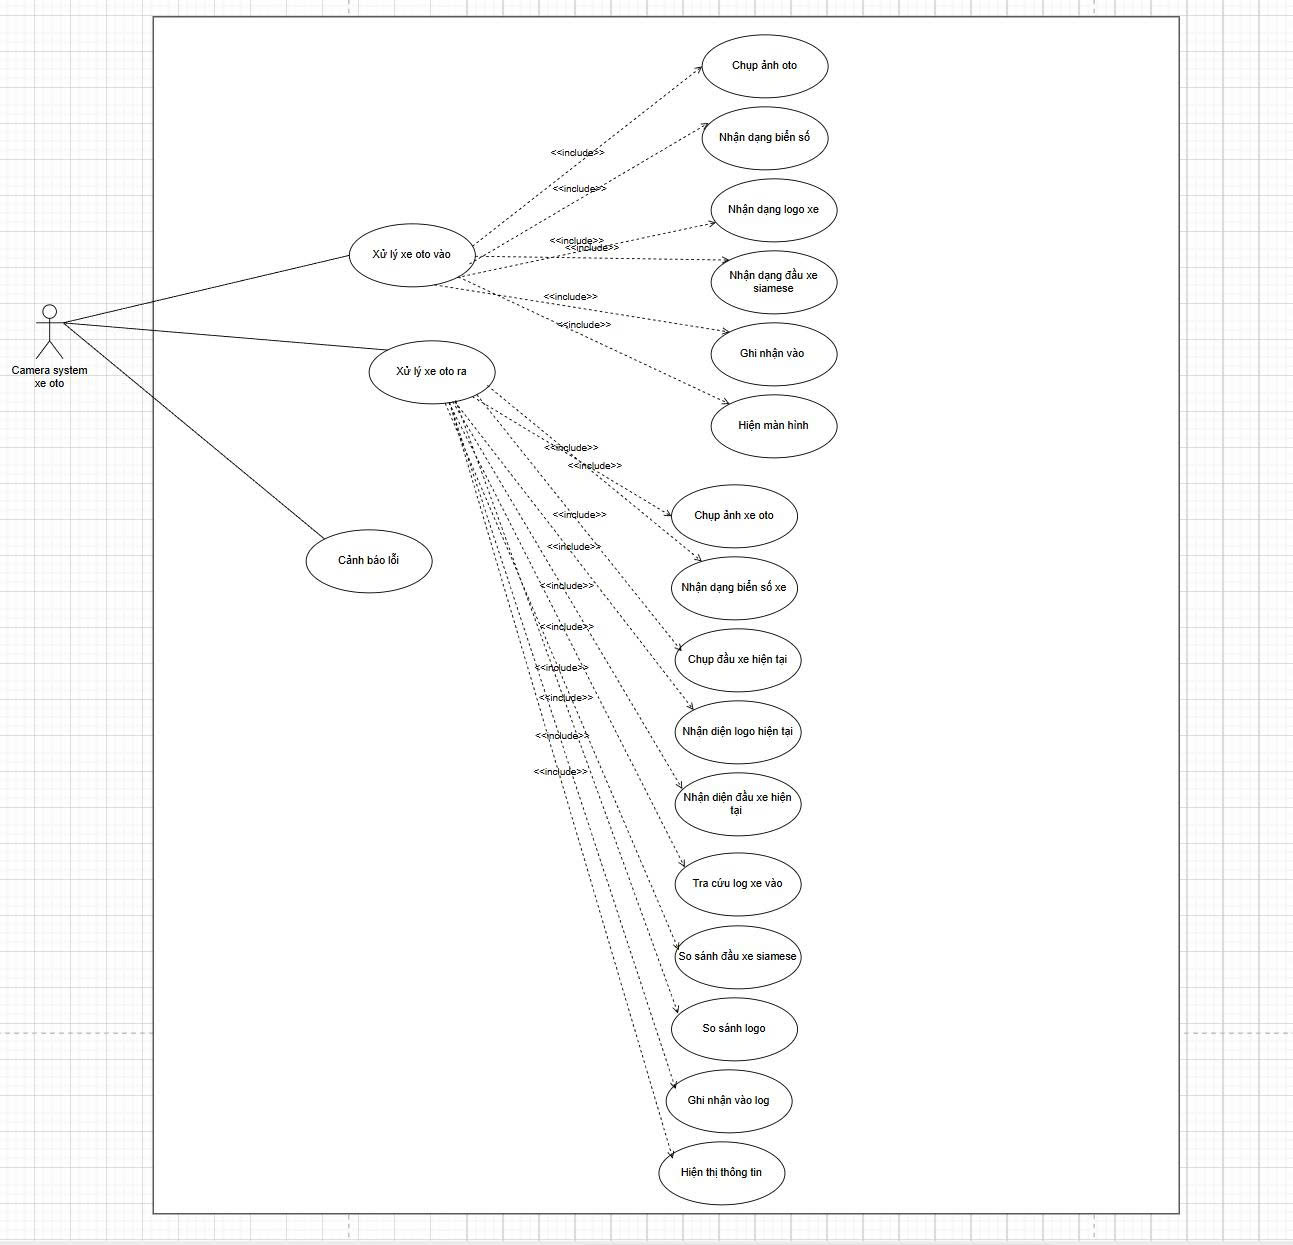
\includegraphics[width=1.0\textwidth]{figures/usecase_xeoto.jpg}
    \caption{Sơ đồ Use Case chi tiết cho camera system xe oto }
    \label{fig:architecture}
\end{figure}




\begin{table}[H]
\caption{Đặc tả UC-06 - Xử lý xe ô tô vào}
\centering
\begin{tabular}{|p{4cm}|p{10cm}|}
\hline
\textbf{Mã Use Case} & UC-06 \\ \hline
\textbf{Tên Use Case} & Xử lý xe ô tô vào \\ \hline
\textbf{Actor} & Camera System Xe Ô Tô \\ \hline
\textbf{Mô tả} & Hệ thống xử lý xe ô tô vào bãi đỗ, bao gồm chụp ảnh, nhận dạng biển số, logo xe, đặc trưng Siamese, ghi nhận vào log và hiển thị thông tin \\ \hline
\textbf{Tiền điều kiện} & Camera hoạt động bình thường, hệ thống AI đã được khởi động \\ \hline
\textbf{Luồng chính} & 
\begin{minipage}[t]{\linewidth}
\begin{enumerate}[leftmargin=*,nosep]
\item Camera phát hiện xe ô tô tiếp cận
\item Hệ thống chụp ảnh ô tô 
\item Nhận dạng biển số 
\item Nhận dạng logo xe 
\item Nhận dạng đặc trưng xe Siamese 
\item Ghi nhận vào log 
\item Hiển thị thông tin trên màn hình 
\end{enumerate}
\end{minipage} \\ \hline
\textbf{Luồng thay thế} & Nếu nhận dạng thất bại, hiển thị lỗi và yêu cầu xử lý thủ công \\ \hline
\textbf{Hậu điều kiện} & Thông tin xe được lưu vào database, ảnh xe được lưu trữ, barrier mở cho xe vào \\ \hline
\end{tabular}
\end{table}


\begin{table}[H]
\caption{Đặc tả UC-07 - Chụp ảnh ô tô}
\centering
\begin{tabular}{|p{4cm}|p{10cm}|}
\hline
\textbf{Mã Use Case} & UC-07 \\ \hline
\textbf{Tên Use Case} & Chụp ảnh ô tô \\ \hline
\textbf{Actor} & Camera System \\ \hline
\textbf{Mô tả} & Chụp ảnh toàn cảnh xe ô tô để lưu trữ và so sánh khi xe ra \\ \hline
\textbf{Tiền điều kiện} & Camera hoạt động, xe trong tầm nhìn camera \\ \hline
\textbf{Luồng chính} & 
\begin{minipage}[t]{\linewidth}
\begin{enumerate}[leftmargin=*,nosep]
\item Camera chụp ảnh xe từ góc phù hợp
\item Kiểm tra chất lượng ảnh
\item Lưu ảnh vào storage
\item Trả về đường dẫn ảnh
\end{enumerate}
\end{minipage} \\ \hline
\textbf{Luồng thay thế} & Nếu ảnh chất lượng kém, chụp lại \\ \hline
\textbf{Hậu điều kiện} & Ảnh xe được lưu thành công \\ \hline
\end{tabular}
\end{table}



\begin{table}[H]
\caption{Đặc tả UC-08 - Nhận dạng biển số xe}
\centering
\begin{tabular}{|p{4cm}|p{10cm}|}
\hline
\textbf{Mã Use Case} & UC-08 \\ \hline
\textbf{Tên Use Case} & Nhận dạng biển số xe \\ \hline
\textbf{Actor} & Hệ thống AI \\ \hline
\textbf{Mô tả} & Sử dụng YOLOv8 và CNN để phát hiện và đọc biển số xe ô tô \\ \hline
\textbf{Tiền điều kiện} & Có ảnh xe chất lượng tốt \\ \hline
\textbf{Luồng chính} & 
\begin{minipage}[t]{\linewidth}
\begin{enumerate}[leftmargin=*,nosep]
\item Nhận ảnh từ camera
\item YOLOv8 phát hiện vị trí biển số
\item CNN nhận diện từng ký tự
\item Trả về chuỗi biển số
\end{enumerate}
\end{minipage} \\ \hline
\textbf{Luồng thay thế} & Nếu không phát hiện được biển số hoặc độ tin cậy thấp, trả về lỗi \\ \hline
\textbf{Hậu điều kiện} & Biển số được trích xuất thành công \\ \hline
\end{tabular}
\end{table}



\begin{table}[H]
\caption{Đặc tả UC-09 - Nhận dạng logo xe}
\centering
\begin{tabular}{|p{4cm}|p{10cm}|}
\hline
\textbf{Mã Use Case} & UC-09 \\ \hline
\textbf{Tên Use Case} & Nhận dạng logo xe \\ \hline
\textbf{Actor} & Hệ thống AI \\ \hline
\textbf{Mô tả} & Sử dụng YOLOv8 để phát hiện và nhận diện logo thương hiệu xe \\ \hline
\textbf{Tiền điều kiện} & Có ảnh xe, logo xe rõ ràng \\ \hline
\textbf{Luồng chính} & 
\begin{minipage}[t]{\linewidth}
\begin{enumerate}[leftmargin=*,nosep]
\item Nhận ảnh xe từ camera
\item YOLOv8 phát hiện vị trí logo
\item Phân loại thương hiệu xe
\item Trả về tên thương hiệu và độ tin cậy
\end{enumerate}
\end{minipage} \\ \hline
\textbf{Luồng thay thế} & Nếu không phát hiện logo hoặc độ tin cậy thấp, bỏ qua bước này \\ \hline
\textbf{Hậu điều kiện} & Thương hiệu xe được xác định  \\ \hline
\end{tabular}
\end{table}


\begin{table}[H]
\caption{Đặc tả UC-10 - Nhận dạng đặc trưng xe Siamese}
\centering
\begin{tabular}{|p{4cm}|p{10cm}|}
\hline
\textbf{Mã Use Case} & UC-10 \\ \hline
\textbf{Tên Use Case} & Nhận dạng đặc trưng xe Siamese \\ \hline
\textbf{Actor} & Hệ thống AI \\ \hline
\textbf{Mô tả} & Sử dụng Siamese Network để trích xuất đặc trưng xe phục vụ so sánh khi xe ra \\ \hline
\textbf{Tiền điều kiện} & Có ảnh xe chất lượng tốt \\ \hline
\textbf{Luồng chính} & 
\begin{minipage}[t]{\linewidth}
\begin{enumerate}[leftmargin=*,nosep]
\item Nhận ảnh xe từ camera
\item Siamese Network trích xuất vector đặc trưng
\item Lưu vector đặc trưng vào database
\item Trả về thông báo thành công
\end{enumerate}
\end{minipage} \\ \hline
\textbf{Luồng thay thế} & Nếu trích xuất thất bại, ghi log lỗi \\ \hline
\textbf{Hậu điều kiện} & Đặc trưng xe được lưu thành công để so sánh sau này \\ \hline
\end{tabular}
\end{table}


\begin{table}[H]
\caption{Đặc tả UC-11 - Xử lý xe ô tô ra}
\centering
\begin{tabular}{|p{4cm}|p{10cm}|}
\hline
\textbf{Mã Use Case} & UC-11 \\ \hline
\textbf{Tên Use Case} & Xử lý xe ô tô ra \\ \hline
\textbf{Actor} & Camera System Xe Ô Tô \\ \hline
\textbf{Mô tả} & Hệ thống xử lý xe ô tô ra khỏi bãi đỗ, so sánh đặc trưng xe, kiểm tra logo \\ \hline
\textbf{Tiền điều kiện} & Xe đang có trong bãi đỗ, camera hoạt động bình thường \\ \hline
\textbf{Luồng chính} & 
\begin{minipage}[t]{\linewidth}
\begin{enumerate}[leftmargin=*,nosep]
\item Camera phát hiện xe ô tô đến cổng ra
\item Chụp ảnh xe ô tô 
\item Nhận dạng biển số xe 
\item Chụp đặc trưng xe hiện tại 
\item Nhận diện logo xe hiện tại 
\item Nhận diện đặc trưng xe hiện tại 
\item Tra cứu thông tin xe vào
\item So sánh đặc trưng xe Siamese 
\item So sánh logo 
\item Ghi nhận vào log 
\item Hiển thị thông tin 
\end{enumerate}
\end{minipage} \\ \hline
\textbf{Luồng thay thế} & 
\begin{minipage}[t]{\linewidth}
\begin{itemize}[leftmargin=*,nosep]
\item Nếu không tìm thấy xe: Hiển thị lỗi
\item Nếu đặc trưng xe không khớp (similarity > 0.5) thì tạo cảnh báo 

\end{itemize}
\end{minipage} \\ \hline
\textbf{Hậu điều kiện} & Phiên đỗ xe kết thúc, barrier mở, thông tin được cập nhật \\ \hline
\end{tabular}
\end{table}



\begin{table}[H]
\caption{Đặc tả UC-12 - So sánh đặc trưng xe Siamese}
\centering
\begin{tabular}{|p{4cm}|p{10cm}|}
\hline
\textbf{Mã Use Case} & UC-12 \\ \hline
\textbf{Tên Use Case} & So sánh đặc trưng xe Siamese \\ \hline
\textbf{Actor} & Hệ thống AI \\ \hline
\textbf{Mô tả} & Sử dụng Siamese Network để so sánh độ tương đồng giữa xe vào và xe ra \\ \hline
\textbf{Tiền điều kiện} & Có ảnh xe vào và xe ra, đã trích xuất được đặc trưng \\ \hline
\textbf{Luồng chính} & 
\begin{minipage}[t]{\linewidth}
\begin{enumerate}[leftmargin=*,nosep]
\item Lấy vector đặc trưng xe vào từ database
\item Trích xuất vector đặc trưng xe ra hiện tại
\item Tính toán độ tương đồng (similarity score)
\item So sánh với ngưỡng (threshold = 0.5)
\item Trả về kết quả khớp/không khớp
\end{enumerate}
\end{minipage} \\ \hline
\textbf{Luồng thay thế} & Nếu similarity > 0.5, trả về không khớp và tạo cảnh báo \\ \hline
\textbf{Hậu điều kiện} & Kết quả so sánh được trả về, quyết định cho xe ra hoặc cảnh báo \\ \hline
\end{tabular}
\end{table}



\begin{table}[H]
\caption{Đặc tả UC-13 - Cảnh báo lỗi}
\centering
\begin{tabular}{|p{4cm}|p{10cm}|}
\hline
\textbf{Mã Use Case} & UC-13 \\ \hline
\textbf{Tên Use Case} & Cảnh báo lỗi \\ \hline
\textbf{Actor} & Camera System Xe Ô Tô \\ \hline
\textbf{Mô tả} & Hệ thống phát hiện bất thường và gửi cảnh báo \\ \hline
\textbf{Tiền điều kiện} & Có sự kiện bất thường xảy ra (đặc trưng xe không khớp, logo không khớp, xe không có trong database) \\ \hline
\textbf{Luồng chính} & 
\begin{minipage}[t]{\linewidth}
\begin{enumerate}[leftmargin=*,nosep]
\item Hệ thống phát hiện bất thường
\item Tạo thông báo cảnh báo chi tiết
\item Gửi cảnh báo đến bảo vệ và chủ xe
\item Ghi log sự kiện
\item Chờ xử lý thủ công
\end{enumerate}
\end{minipage} \\ \hline
\textbf{Hậu điều kiện} & Cảnh báo được ghi nhận, chờ bảo vệ hoặc chủ xe xử lý \\ \hline
\end{tabular}
\end{table}



\subsection{Sơ đồ Use Case chi tiết cho người dùng app mobile }

\begin{figure}[H]
    \centering
    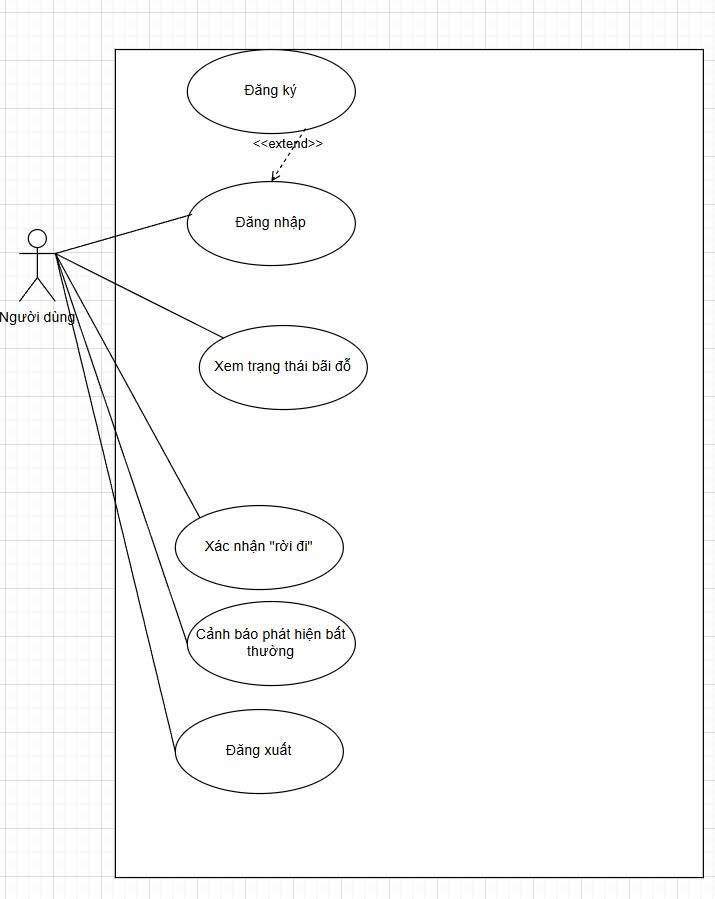
\includegraphics[width=0.95\textwidth]{figures/usecasse_user.jpg}
    \caption{Sơ đồ Use Case chi tiết người dùng app mobile }
    \label{fig:architecture}
\end{figure}




\begin{table}[H]
\caption{Đặc tả UC-14 - Đăng ký}
\centering
\begin{tabular}{|p{4cm}|p{10cm}|}
\hline
\textbf{Mã Use Case} & UC-14 \\ \hline
\textbf{Tên Use Case} & Đăng ký \\ \hline
\textbf{Actor} & Người dùng \\ \hline
\textbf{Mô tả} & Người dùng tạo tài khoản mới trong hệ thống \\ \hline
\textbf{Tiền điều kiện} & Người dùng chưa có tài khoản, có kết nối internet \\ \hline
\textbf{Luồng chính} & 
\begin{minipage}[t]{\linewidth}
\begin{enumerate}[leftmargin=*,nosep]
\item Người dùng mở ứng dụng và chọn "Đăng ký"
\item Nhập thông tin: họ tên, email, mật khẩu
\item Hệ thống kiểm tra tính hợp lệ dữ liệu
\item Hệ thống kiểm tra email đã tồn tại chưa
\item Tạo tài khoản mới
\item Hiển thị thông báo đăng ký thành công
\item Chuyển đến màn hình đăng nhập
\end{enumerate}
\end{minipage} \\ \hline
\textbf{Luồng thay thế} & 
\begin{minipage}[t]{\linewidth}
\begin{itemize}[leftmargin=*,nosep]
\item Nếu email đã tồn tại: Hiển thị lỗi "Email đã được sử dụng"
\item Nếu dữ liệu không hợp lệ: Hiển thị thông báo lỗi cụ thể
\item Nếu mất kết nối: Hiển thị lỗi kết nối
\end{itemize}
\end{minipage} \\ \hline
\textbf{Hậu điều kiện} & Tài khoản mới được tạo trong database \\ \hline
\end{tabular}
\end{table}



\begin{table}[H]
\caption{Đặc tả UC-15 - Đăng nhập}
\centering
\begin{tabular}{|p{4cm}|p{10cm}|}
\hline
\textbf{Mã Use Case} & UC-15 \\ \hline
\textbf{Tên Use Case} & Đăng nhập (extend từ UC-14) \\ \hline
\textbf{Actor} & Người dùng \\ \hline
\textbf{Mô tả} & Người dùng đăng nhập vào hệ thống để sử dụng các chức năng \\ \hline
\textbf{Tiền điều kiện} & Người dùng đã có tài khoản, có kết nối internet \\ \hline
\textbf{Luồng chính} & 
\begin{minipage}[t]{\linewidth}
\begin{enumerate}[leftmargin=*,nosep]
\item Người dùng mở ứng dụng
\item Nhập email và mật khẩu
\item Hệ thống xác thực thông tin
\item Tạo phiên đăng nhập (session/token)
\item Lưu token vào local storage
\item Chuyển đến trang chủ
\end{enumerate}
\end{minipage} \\ \hline
\textbf{Luồng thay thế} & 
\begin{minipage}[t]{\linewidth}
\begin{itemize}[leftmargin=*,nosep]
\item Nếu sai email/mật khẩu: Hiển thị "Thông tin đăng nhập không chính xác"
\item Nếu tài khoản bị khóa: Hiển thị thông báo và hướng dẫn
\item Nếu quên mật khẩu: Chuyển đến màn hình đặt lại mật khẩu
\end{itemize}
\end{minipage} \\ \hline
\textbf{Hậu điều kiện} & Người dùng đăng nhập thành công, có quyền truy cập các chức năng \\ \hline
\end{tabular}
\end{table}



\begin{table}[H]
\caption{Đặc tả UC-16 - Xem trạng thái bãi đỗ}
\centering
\begin{tabular}{|p{4cm}|p{10cm}|}
\hline
\textbf{Mã Use Case} & UC-16 \\ \hline
\textbf{Tên Use Case} & Xem trạng thái bãi đỗ \\ \hline
\textbf{Actor} & Người dùng \\ \hline
\textbf{Mô tả} & Người dùng xem thông tin các xe đang đỗ trong bãi của mình \\ \hline
\textbf{Tiền điều kiện} & Người dùng đã đăng nhập, có ít nhất một xe đã đăng ký \\ \hline
\textbf{Luồng chính} & 
\begin{minipage}[t]{\linewidth}
\begin{enumerate}[leftmargin=*,nosep]
\item Người dùng chọn "Xe của tôi" hoặc "Trạng thái bãi đỗ"
\item Hệ thống lấy danh sách xe đang đỗ của người dùng
\item Hiển thị danh sách: biển số, loại xe, thời gian vào, vị trí
\item Cập nhật real-time khi có thay đổi
\end{enumerate}
\end{minipage} \\ \hline
\textbf{Luồng thay thế} & Nếu không có xe nào đang đỗ: Hiển thị "Bạn chưa có xe nào trong bãi" \\ \hline
\textbf{Hậu điều kiện} & Người dùng xem được thông tin xe đang đỗ \\ \hline
\end{tabular}
\end{table}



\begin{table}[H]
\caption{Đặc tả UC-17 - Xác nhận "rời đi"}
\centering
\begin{tabular}{|p{4cm}|p{10cm}|}
\hline
\textbf{Mã Use Case} & UC-17 \\ \hline
\textbf{Tên Use Case} & Xác nhận "rời đi" \\ \hline
\textbf{Actor} & Người dùng \\ \hline
\textbf{Mô tả} & Người dùng xác nhận sẽ lấy xe ra khỏi bãi đỗ \\ \hline
\textbf{Tiền điều kiện} & Có ít nhất một xe đang đỗ trong bãi \\ \hline
\textbf{Luồng chính} & 
\begin{minipage}[t]{\linewidth}
\begin{enumerate}[leftmargin=*,nosep]
\item Người dùng vào màn hình "Xe của tôi"
\item Chọn xe cần lấy ra
\item Nhấn nút "Xác nhận rời đi"

\item Gửi thông báo đến hệ thống camera
\end{enumerate}
\end{minipage} \\ \hline
\textbf{Luồng thay thế} & 
\begin{minipage}[t]{\linewidth}
\begin{itemize}[leftmargin=*,nosep]
\item Nếu hết thời gian hiệu lực: Yêu cầu xác nhận lại
\item Nếu xe đã được xác nhận: Hiển thị "Xe đã được xác nhận rời đi"
\end{itemize}
\end{minipage} \\ \hline
\textbf{Hậu điều kiện} & Hệ thống ghi nhận xác nhận, cho phép xe ra khi camera phát hiện \\ \hline
\end{tabular}
\end{table}



\begin{table}[H]
\caption{Đặc tả UC-18 - Cảnh báo phát hiện bất thường}
\centering
\begin{tabular}{|p{4cm}|p{10cm}|}
\hline
\textbf{Mã Use Case} & UC-18 \\ \hline
\textbf{Tên Use Case} & Cảnh báo phát hiện bất thường \\ \hline
\textbf{Actor} & Người dùng \\ \hline
\textbf{Mô tả} & Người dùng nhận cảnh báo khi hệ thống phát hiện bất thường về xe của mình \\ \hline
\textbf{Tiền điều kiện} & Hệ thống phát hiện bất thường (khuôn mặt không khớp, xe không khớp, xe vào/ra không xác nhận) \\ \hline
\textbf{Luồng chính} & 
\begin{minipage}[t]{\linewidth}
\begin{enumerate}[leftmargin=*,nosep]
\item Hệ thống phát hiện bất thường
\item Gửi push notification đến điện thoại người dùng
\item Người dùng mở thông báo
\item Hiển thị chi tiết: loại cảnh báo, thời gian, ảnh/video
\item Người dùng xác nhận "Đó là tôi" hoặc "Không phải tôi"
\item Hệ thống ghi nhận phản hồi
\item Cập nhật trạng thái cảnh báo
\end{enumerate}
\end{minipage} \\ \hline
\textbf{Luồng thay thế} & 
\begin{minipage}[t]{\linewidth}
\begin{itemize}[leftmargin=*,nosep]
\item Nếu không phản hồi trong thời gian quy định: Barrier giữ đóng, thông báo bảo vệ
\item Nếu xác nhận "Không phải tôi": Tạo báo cáo khẩn cấp, thông báo bảo vệ
\end{itemize}
\end{minipage} \\ \hline
\textbf{Hậu điều kiện} & Cảnh báo được xử lý, quyết định cho xe ra hoặc giữ lại \\ \hline
\end{tabular}
\end{table}


\begin{table}[H]
\caption{Đặc tả UC-19 - Đăng xuất}
\centering
\begin{tabular}{|p{4cm}|p{10cm}|}
\hline
\textbf{Mã Use Case} & UC-19 \\ \hline
\textbf{Tên Use Case} & Đăng xuất \\ \hline
\textbf{Actor} & Người dùng \\ \hline
\textbf{Mô tả} & Người dùng đăng xuất khỏi ứng dụng \\ \hline
\textbf{Tiền điều kiện} & Người dùng đã đăng nhập \\ \hline
\textbf{Luồng chính} & 
\begin{minipage}[t]{\linewidth}
\begin{enumerate}[leftmargin=*,nosep]
\item Người dùng vào menu "Tài khoản"
\item Chọn "Đăng xuất"
\item Hiển thị xác nhận "Bạn có chắc muốn đăng xuất?"
\item Người dùng xác nhận
\item Hệ thống xóa token khỏi local storage
\item Hủy phiên đăng nhập
\item Chuyển về màn hình đăng nhập
\end{enumerate}
\end{minipage} \\ \hline
\textbf{Luồng thay thế} & Nếu người dùng chọn "Hủy": Quay lại màn hình trước \\ \hline
\textbf{Hậu điều kiện} & Người dùng đã đăng xuất, phải đăng nhập lại để sử dụng \\ \hline
\end{tabular}
\end{table}



\subsection{Sơ đồ Use Case chi tiết cho bảo vệ}
\begin{figure}[H]
    \centering
    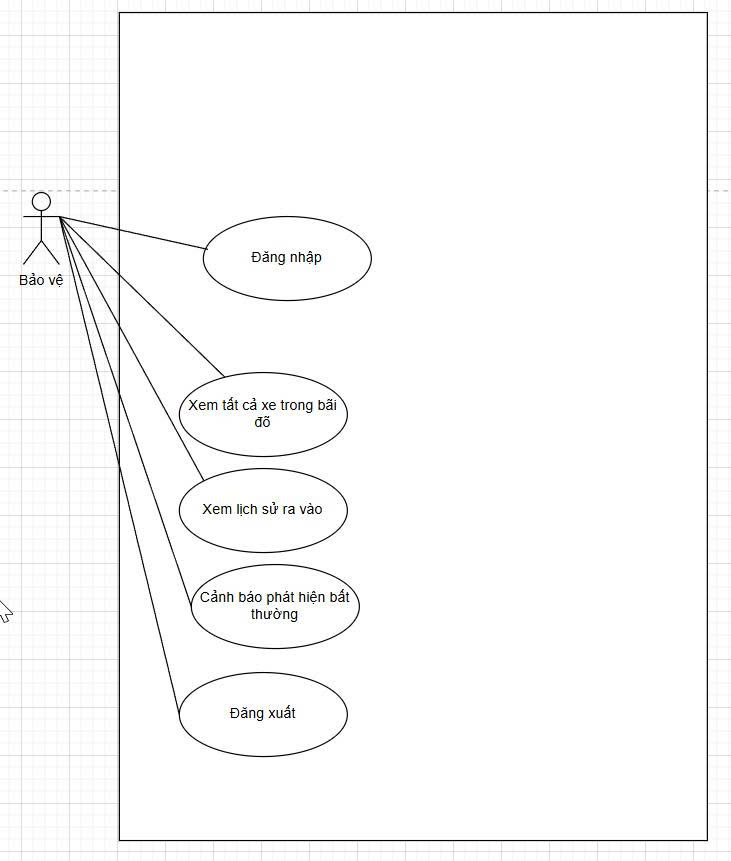
\includegraphics[width=1.0\textwidth]{figures/usecase_baove.jpg}
    \caption{Sơ đồ Use Case chi tiết bảo vệ }
    \label{fig:architecture}
\end{figure}


\begin{table}[H]
\caption{Đặc tả UC-20 - Đăng nhập (Bảo vệ)}
\centering
\begin{tabular}{|p{4cm}|p{10cm}|}
\hline
\textbf{Mã Use Case} & UC-20 \\ \hline
\textbf{Tên Use Case} & Đăng nhập \\ \hline
\textbf{Actor} & Bảo vệ \\ \hline
\textbf{Mô tả} & Bảo vệ đăng nhập vào ứng dụng để giám sát và quản lý bãi đỗ \\ \hline
\textbf{Tiền điều kiện} & Bảo vệ đã có tài khoản được cấp bởi quản trị viên, có kết nối internet \\ \hline
\textbf{Luồng chính} & 
\begin{minipage}[t]{\linewidth}
\begin{enumerate}[leftmargin=*,nosep]
\item Bảo vệ mở ứng dụng
\item Nhập tên đăng nhập và mật khẩu
\item Hệ thống xác thực thông tin
\item Kiểm tra quyền truy cập của bảo vệ
\item Lưu token vào local storage
\item Chuyển đến trang chủ giám sát
\end{enumerate}
\end{minipage} \\ \hline
\textbf{Luồng thay thế} & 
\begin{minipage}[t]{\linewidth}
\begin{itemize}[leftmargin=*,nosep]
\item Nếu sai thông tin đăng nhập: Hiển thị "Thông tin không chính xác"
\item Nếu tài khoản bị khóa: Hiển thị thông báo liên hệ quản trị viên

\end{itemize}
\end{minipage} \\ \hline
\textbf{Hậu điều kiện} & Bảo vệ đăng nhập thành công, có quyền truy cập các chức năng giám sát \\ \hline
\end{tabular}
\end{table}



\begin{table}[H]
\caption{Đặc tả UC-21 - Xem tất cả xe trong bãi đỗ}
\centering
\begin{tabular}{|p{4cm}|p{10cm}|}
\hline
\textbf{Mã Use Case} & UC-21 \\ \hline
\textbf{Tên Use Case} & Xem tất cả xe trong bãi đỗ \\ \hline
\textbf{Actor} & Bảo vệ \\ \hline
\textbf{Mô tả} & Bảo vệ xem danh sách tất cả xe đang đỗ trong bãi với thông tin chi tiết \\ \hline
\textbf{Tiền điều kiện} & Bảo vệ đã đăng nhập \\ \hline
\textbf{Luồng chính} & 
\begin{minipage}[t]{\linewidth}
\begin{enumerate}[leftmargin=*,nosep]
\item Bảo vệ chọn "Xe trong bãi" từ menu chính
\item Hệ thống lấy danh sách tất cả xe đang đỗ
\item Hiển thị thông tin: biển số, loại xe, chủ xe, thời gian vào, vị trí, ảnh xe
\item Cập nhật real-time khi có xe vào/ra
\item Bảo vệ có thể tìm kiếm theo biển số
\item Bảo vệ có thể lọc theo loại xe, khu vực
\item Chọn xe để xem chi tiết
\end{enumerate}
\end{minipage} \\ \hline
\textbf{Luồng thay thế} & 
\begin{minipage}[t]{\linewidth}
\begin{itemize}[leftmargin=*,nosep]
\item Nếu bãi đỗ trống: Hiển thị "Hiện không có xe nào trong bãi"
\item Nếu mất kết nối: Hiển thị lỗi và thử kết nối lại
\end{itemize}
\end{minipage} \\ \hline
\textbf{Hậu điều kiện} & Bảo vệ nắm được tình trạng xe trong bãi đỗ \\ \hline
\end{tabular}
\end{table}


\begin{table}[H]
\caption{Đặc tả UC-22 - Xem lịch sử ra vào}
\centering
\begin{tabular}{|p{4cm}|p{10cm}|}
\hline
\textbf{Mã Use Case} & UC-22 \\ \hline
\textbf{Tên Use Case} & Xem lịch sử ra vào \\ \hline
\textbf{Actor} & Bảo vệ \\ \hline
\textbf{Mô tả} & Bảo vệ tra cứu lịch sử xe vào/ra bãi đỗ theo thời gian \\ \hline
\textbf{Tiền điều kiện} & Bảo vệ đã đăng nhập, hệ thống có dữ liệu lịch sử \\ \hline
\textbf{Luồng chính} & 
\begin{minipage}[t]{\linewidth}
\begin{enumerate}[leftmargin=*,nosep]
\item Bảo vệ chọn "Lịch sử ra vào"
\item Chọn khoảng thời gian (hôm nay, tuần này, tháng này, tùy chỉnh)
\item Hệ thống lấy dữ liệu lịch sử
\item Hiển thị danh sách: biển số, loại xe, thời gian vào, thời gian ra, thời gian đỗ, ảnh
\item Bảo vệ có thể tìm kiếm theo biển số cụ thể
\item Chọn bản ghi để xem chi tiết đầy đủ
\item Xem ảnh/video khi xe vào và ra
\end{enumerate}
\end{minipage} \\ \hline
\textbf{Luồng thay thế} & 
\begin{minipage}[t]{\linewidth}
\begin{itemize}[leftmargin=*,nosep]
\item Nếu không có dữ liệu trong khoảng thời gian: Hiển thị "Không có dữ liệu"
\item Nếu tìm kiếm không có kết quả: Hiển thị "Không tìm thấy xe với biển số này"
\end{itemize}
\end{minipage} \\ \hline
\textbf{Hậu điều kiện} & Bảo vệ xem được lịch sử chi tiết các xe ra vào \\ \hline
\end{tabular}
\end{table}


\begin{table}[H]
\caption{Đặc tả UC-23 - Cảnh báo phát hiện bất thường (Bảo vệ)}
\centering
\begin{tabular}{|p{4cm}|p{10cm}|}
\hline
\textbf{Mã Use Case} & UC-23 \\ \hline
\textbf{Tên Use Case} & Cảnh báo phát hiện bất thường \\ \hline
\textbf{Actor} & Bảo vệ \\ \hline
\textbf{Mô tả} & Bảo vệ nhận và xử lý cảnh báo bất thường từ hệ thống \\ \hline
\textbf{Tiền điều kiện} & Hệ thống phát hiện bất thường (nhận dạng thất bại, xe không khớp, không có xác nhận rời đi) \\ \hline
\textbf{Luồng chính} & 
\begin{minipage}[t]{\linewidth}
\begin{enumerate}[leftmargin=*,nosep]
\item Hệ thống phát hiện bất thường
\item Gửi push notification khẩn cấp đến điện thoại bảo vệ
\item Bảo vệ mở thông báo
\item Hiển thị chi tiết cảnh báo: loại, thời gian, biển số, ảnh/video, độ tương đồng (nếu có)
\item Bảo vệ xem xét thông tin
\item Bảo vệ quyết định: "Cho phép ra" hoặc "Giữ lại xe"
\item Xác nhận quyết định
\item Hệ thống cập nhật trạng thái cảnh báo
\item Gửi lệnh đến barrier (mở/đóng)
\item Ghi log sự kiện
\end{enumerate}
\end{minipage} \\ \hline
\textbf{Luồng thay thế} & 
\begin{minipage}[t]{\linewidth}
\begin{itemize}[leftmargin=*,nosep]
\item Nếu bảo vệ không phản hồi trong 3 phút: Barrier giữ đóng, leo thang cảnh báo
\item Nếu cần thêm thông tin: Gọi điện cho chủ xe để xác minh
\item Nếu phát hiện gian lận: Báo cáo lên cấp trên, giữ xe lại
\end{itemize}
\end{minipage} \\ \hline
\textbf{Hậu điều kiện} & Cảnh báo được xử lý, quyết định cho xe ra hoặc giữ lại được thực hiện, log được ghi nhận \\ \hline
\end{tabular}
\end{table}



\begin{table}[H]
\caption{Đặc tả UC-24 - Đăng xuất (Bảo vệ)}
\centering
\begin{tabular}{|p{4cm}|p{10cm}|}
\hline
\textbf{Mã Use Case} & UC-24 \\ \hline
\textbf{Tên Use Case} & Đăng xuất \\ \hline
\textbf{Actor} & Bảo vệ \\ \hline
\textbf{Mô tả} & Bảo vệ đăng xuất khỏi ca làm việc \\ \hline
\textbf{Tiền điều kiện} & Bảo vệ đã đăng nhập \\ \hline
\textbf{Luồng chính} & 
\begin{minipage}[t]{\linewidth}
\begin{enumerate}[leftmargin=*,nosep]
\item Bảo vệ chọn menu "Tài khoản"
\item Chọn "Đăng xuất"
\item Hiển thị xác nhận "Bạn có chắc muốn kết thúc ca làm việc?"
\item Bảo vệ xác nhận
\item Hệ thống ghi nhận thời gian kết thúc ca
\item Xóa token khỏi local storage
\item Hủy phiên làm việc
\item Chuyển về màn hình đăng nhập
\end{enumerate}
\end{minipage} \\ \hline
\textbf{Luồng thay thế} & 
\begin{minipage}[t]{\linewidth}
\begin{itemize}[leftmargin=*,nosep]
\item Nếu còn cảnh báo chưa xử lý: Cảnh báo "Còn X cảnh báo chưa xử lý"
\item Nếu chọn "Hủy": Quay lại màn hình trước
\end{itemize}
\end{minipage} \\ \hline
\textbf{Hậu điều kiện} & Ca làm việc kết thúc, bảo vệ đã đăng xuất \\ \hline
\end{tabular}
\end{table}


\section{Sơ đồ Activity}
\subsection{Sơ đồ Activity người dùng đăng ký đăng nhập}
\begin{figure}[H]
    \centering
    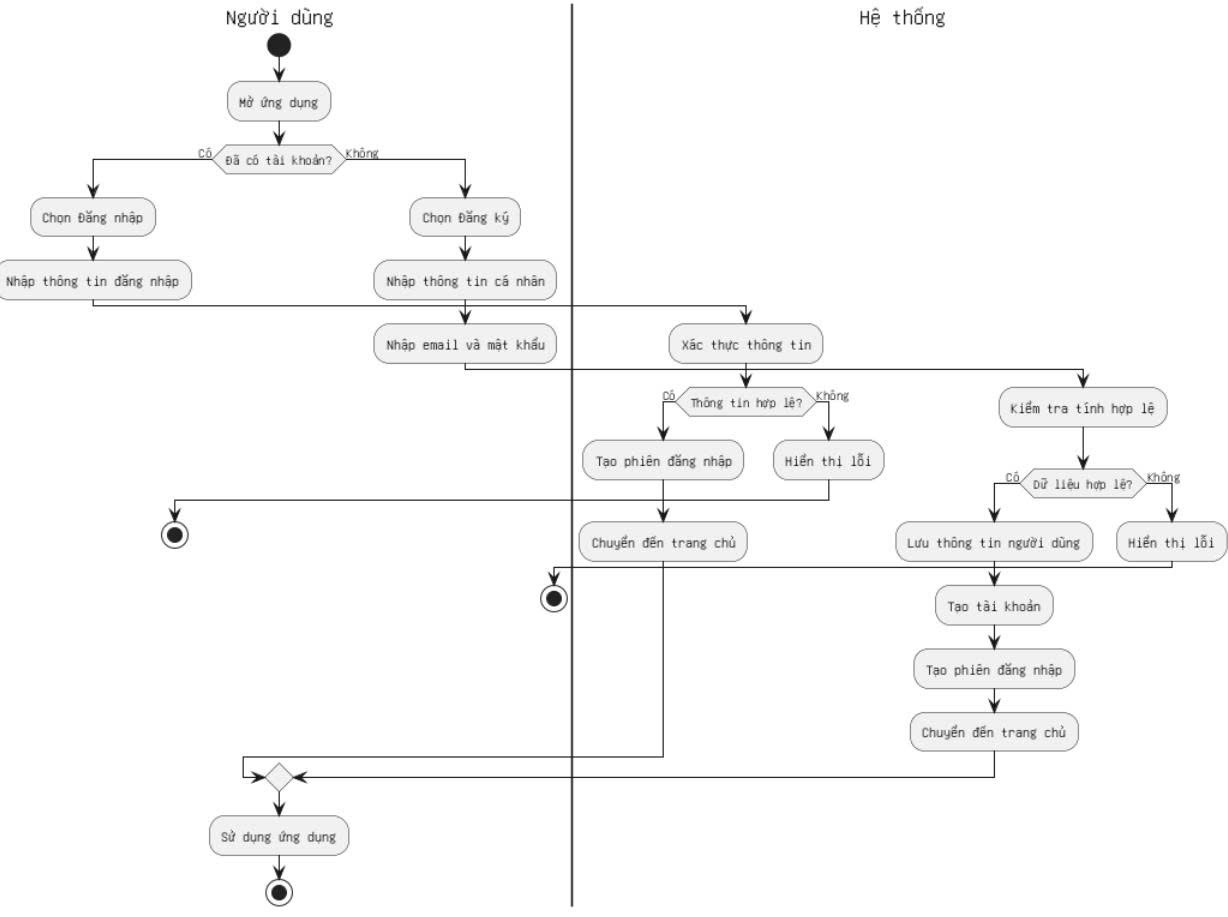
\includegraphics[width=1.0\textwidth]{figures/ac_dkdn.jpg}
    \caption{Sơ đồ Activity người dùng đăng ký đăng nhập}
    \label{fig:architecture}
\end{figure}


Activity diagram mô tả quy trình đăng ký và đăng nhập của người dùng vào hệ thống, bao gồm các bước xác thực thông tin, xử lý dữ liệu và thông báo lỗi.

Luồng xử lý bắt đầu khi người dùng mở ứng dụng và lựa chọn đăng nhập hoặc đăng ký tài khoản.  
Đối với đăng nhập, người dùng nhập email và mật khẩu, hệ thống tiến hành xác thực thông tin. Nếu thông tin hợp lệ, hệ thống tạo phiên đăng nhập và chuyển người dùng đến trang chủ; ngược lại, hệ thống hiển thị thông báo lỗi và yêu cầu nhập lại.

Đối với đăng ký, người dùng nhập thông tin cá nhân cần thiết, hệ thống kiểm tra tính hợp lệ của dữ liệu và xác nhận email chưa tồn tại trong hệ thống. Nếu thỏa điều kiện, hệ thống tạo tài khoản mới, khởi tạo phiên đăng nhập và chuyển đến trang chủ. Trường hợp dữ liệu không hợp lệ hoặc email đã tồn tại, hệ thống hiển thị lỗi và yêu cầu người dùng nhập lại thông tin.

Kết quả cuối cùng của activity là người dùng truy cập thành công vào hệ thống với phiên đăng nhập hợp lệ hoặc nhận thông báo lỗi khi thao tác không thành công.

\subsection{Sơ đồ Activity xử lý xe máy vào bãi đỗ}
\begin{figure}[H]
    \centering
    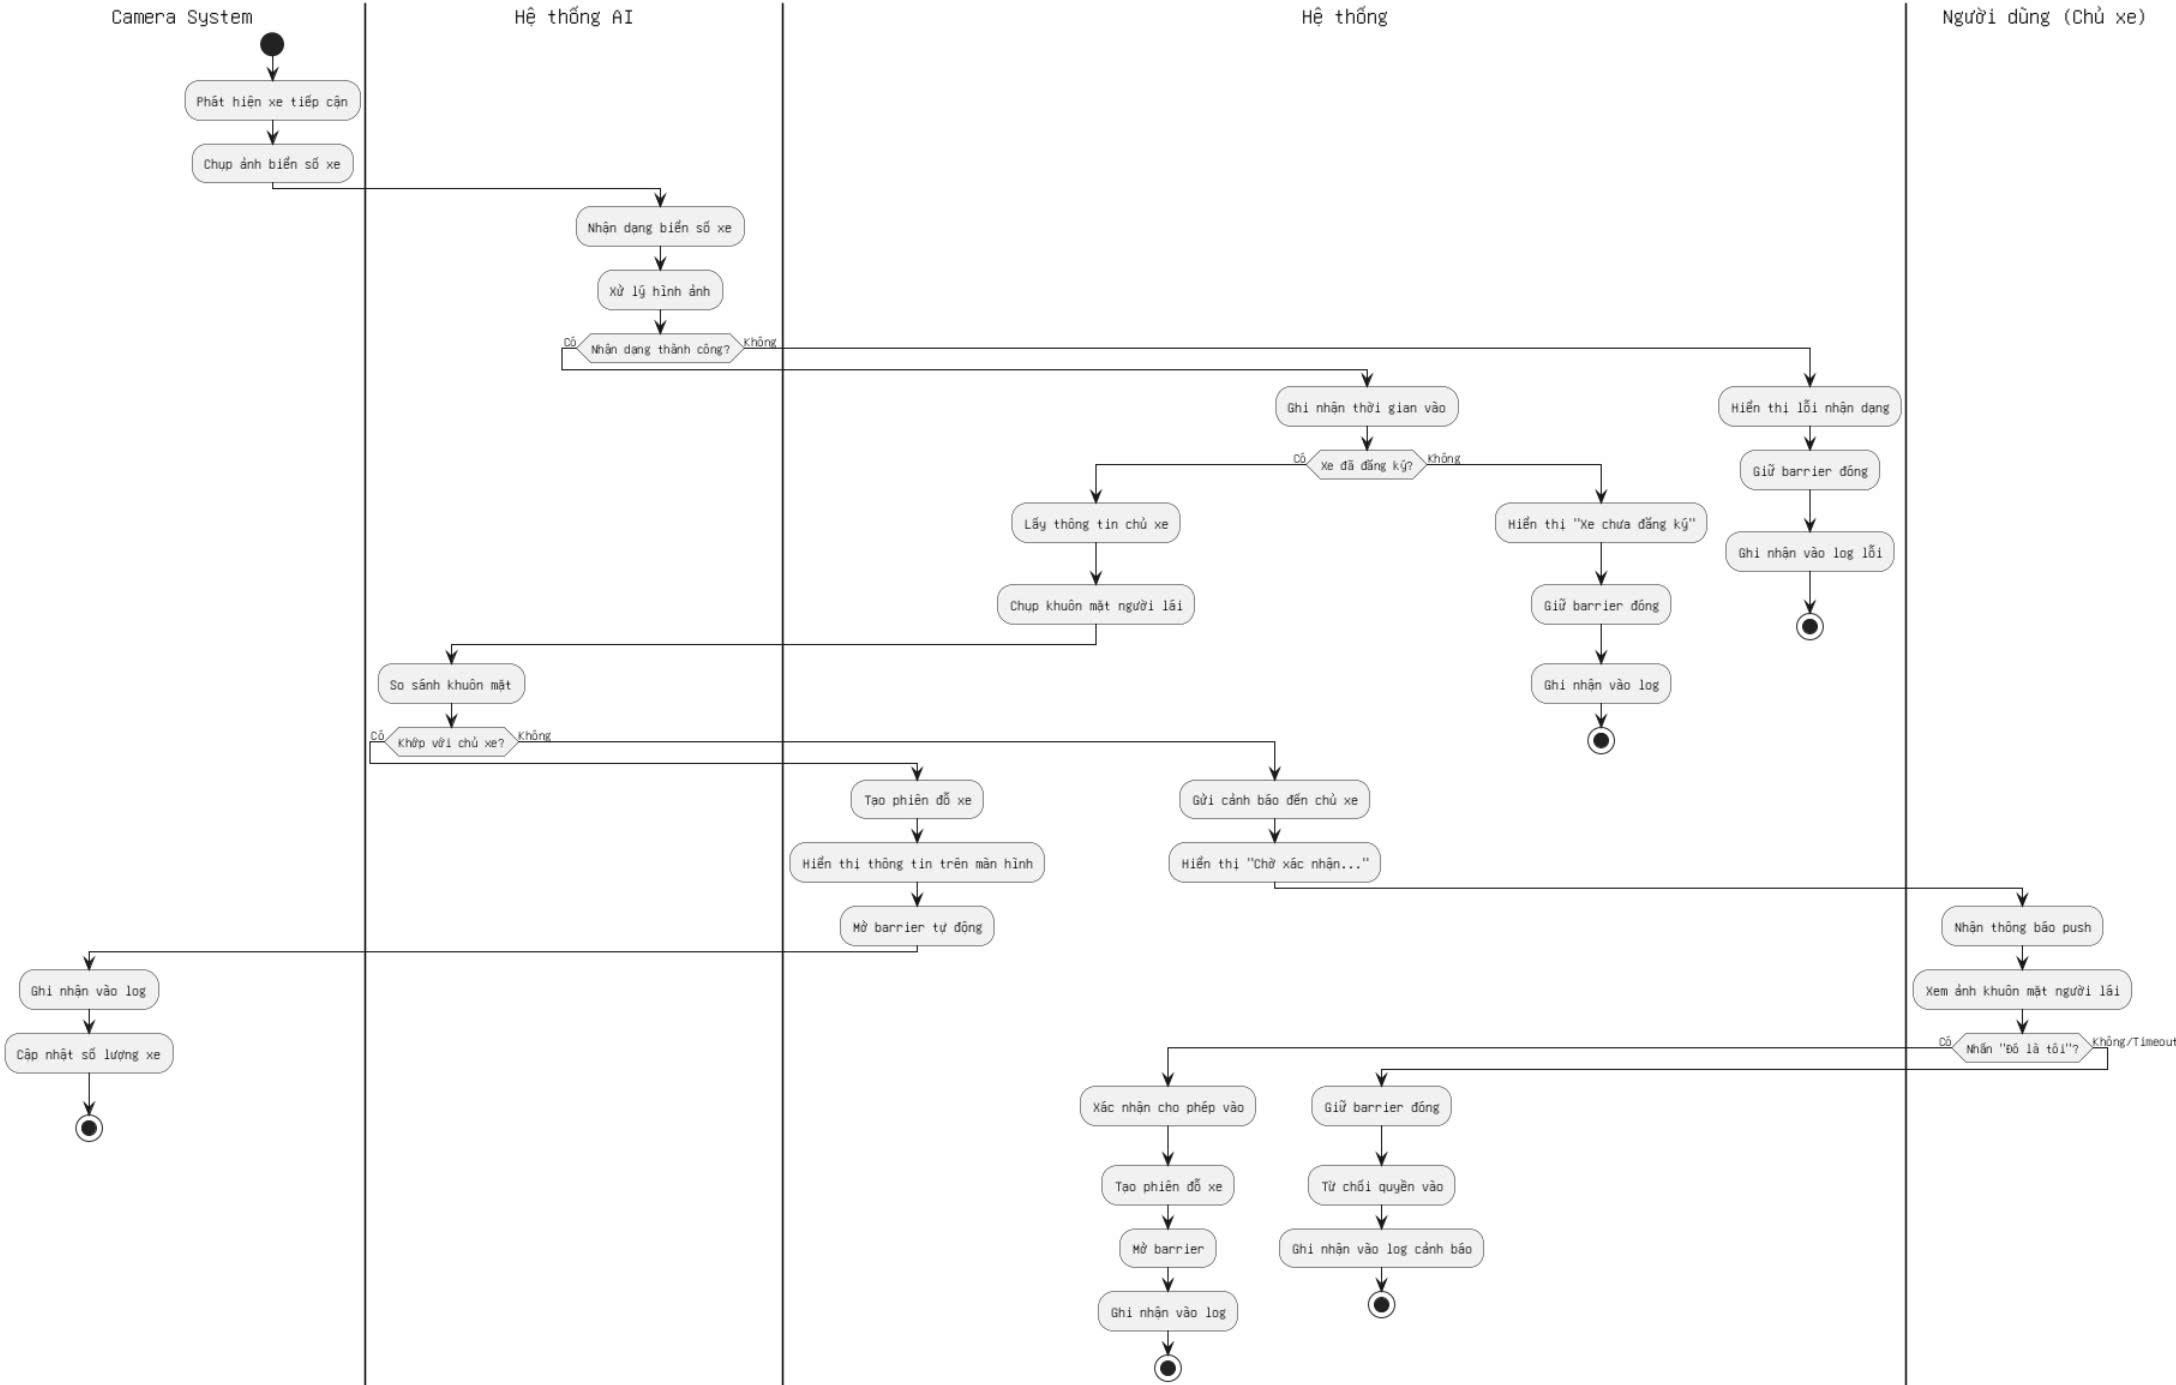
\includegraphics[width=1.0\textwidth]{figures/ac_xemay_vao.jpg}
    \caption{Sơ đồ Activity xử lý xe máy vào bãi đỗ}
    \label{fig:architecture}
\end{figure}
Mục đích: Activity diagram mô tả quy trình xử lý xe máy vào bãi đỗ, bao gồm nhận diện biển số xe, xác thực khuôn mặt người lái và quyết định cho phép xe vào bãi.

Luồng xử lý bắt đầu khi camera phát hiện xe tiếp cận và chụp ảnh biển số. Hệ thống AI tiến hành nhận dạng biển số và kiểm tra tính hợp lệ. Nếu nhận dạng thất bại hoặc xe chưa đăng ký, hệ thống hiển thị lỗi, giữ barrier đóng và ghi nhận log.

Trong trường hợp nhận dạng thành công, hệ thống ghi nhận thời gian vào, lấy thông tin chủ xe và chụp khuôn mặt người lái để so sánh với dữ liệu trong cơ sở dữ liệu. Nếu khuôn mặt khớp với chủ xe, hệ thống tạo phiên đỗ xe và mở barrier tự động.

Nếu khuôn mặt không khớp, hệ thống tạo cảnh báo, gửi thông báo đến chủ xe và yêu cầu xác nhận. Dựa trên phản hồi của chủ xe, hệ thống quyết định cho phép xe vào bãi hoặc từ chối, đồng thời ghi nhận log tương ứng. Quy trình kết thúc khi barrier được mở hoặc giữ đóng và dữ liệu được cập nhật vào hệ thống.


\subsection{Sơ đồ Activity xử lý xe oto vào bãi đỗ}
\begin{figure}[H]
    \centering
    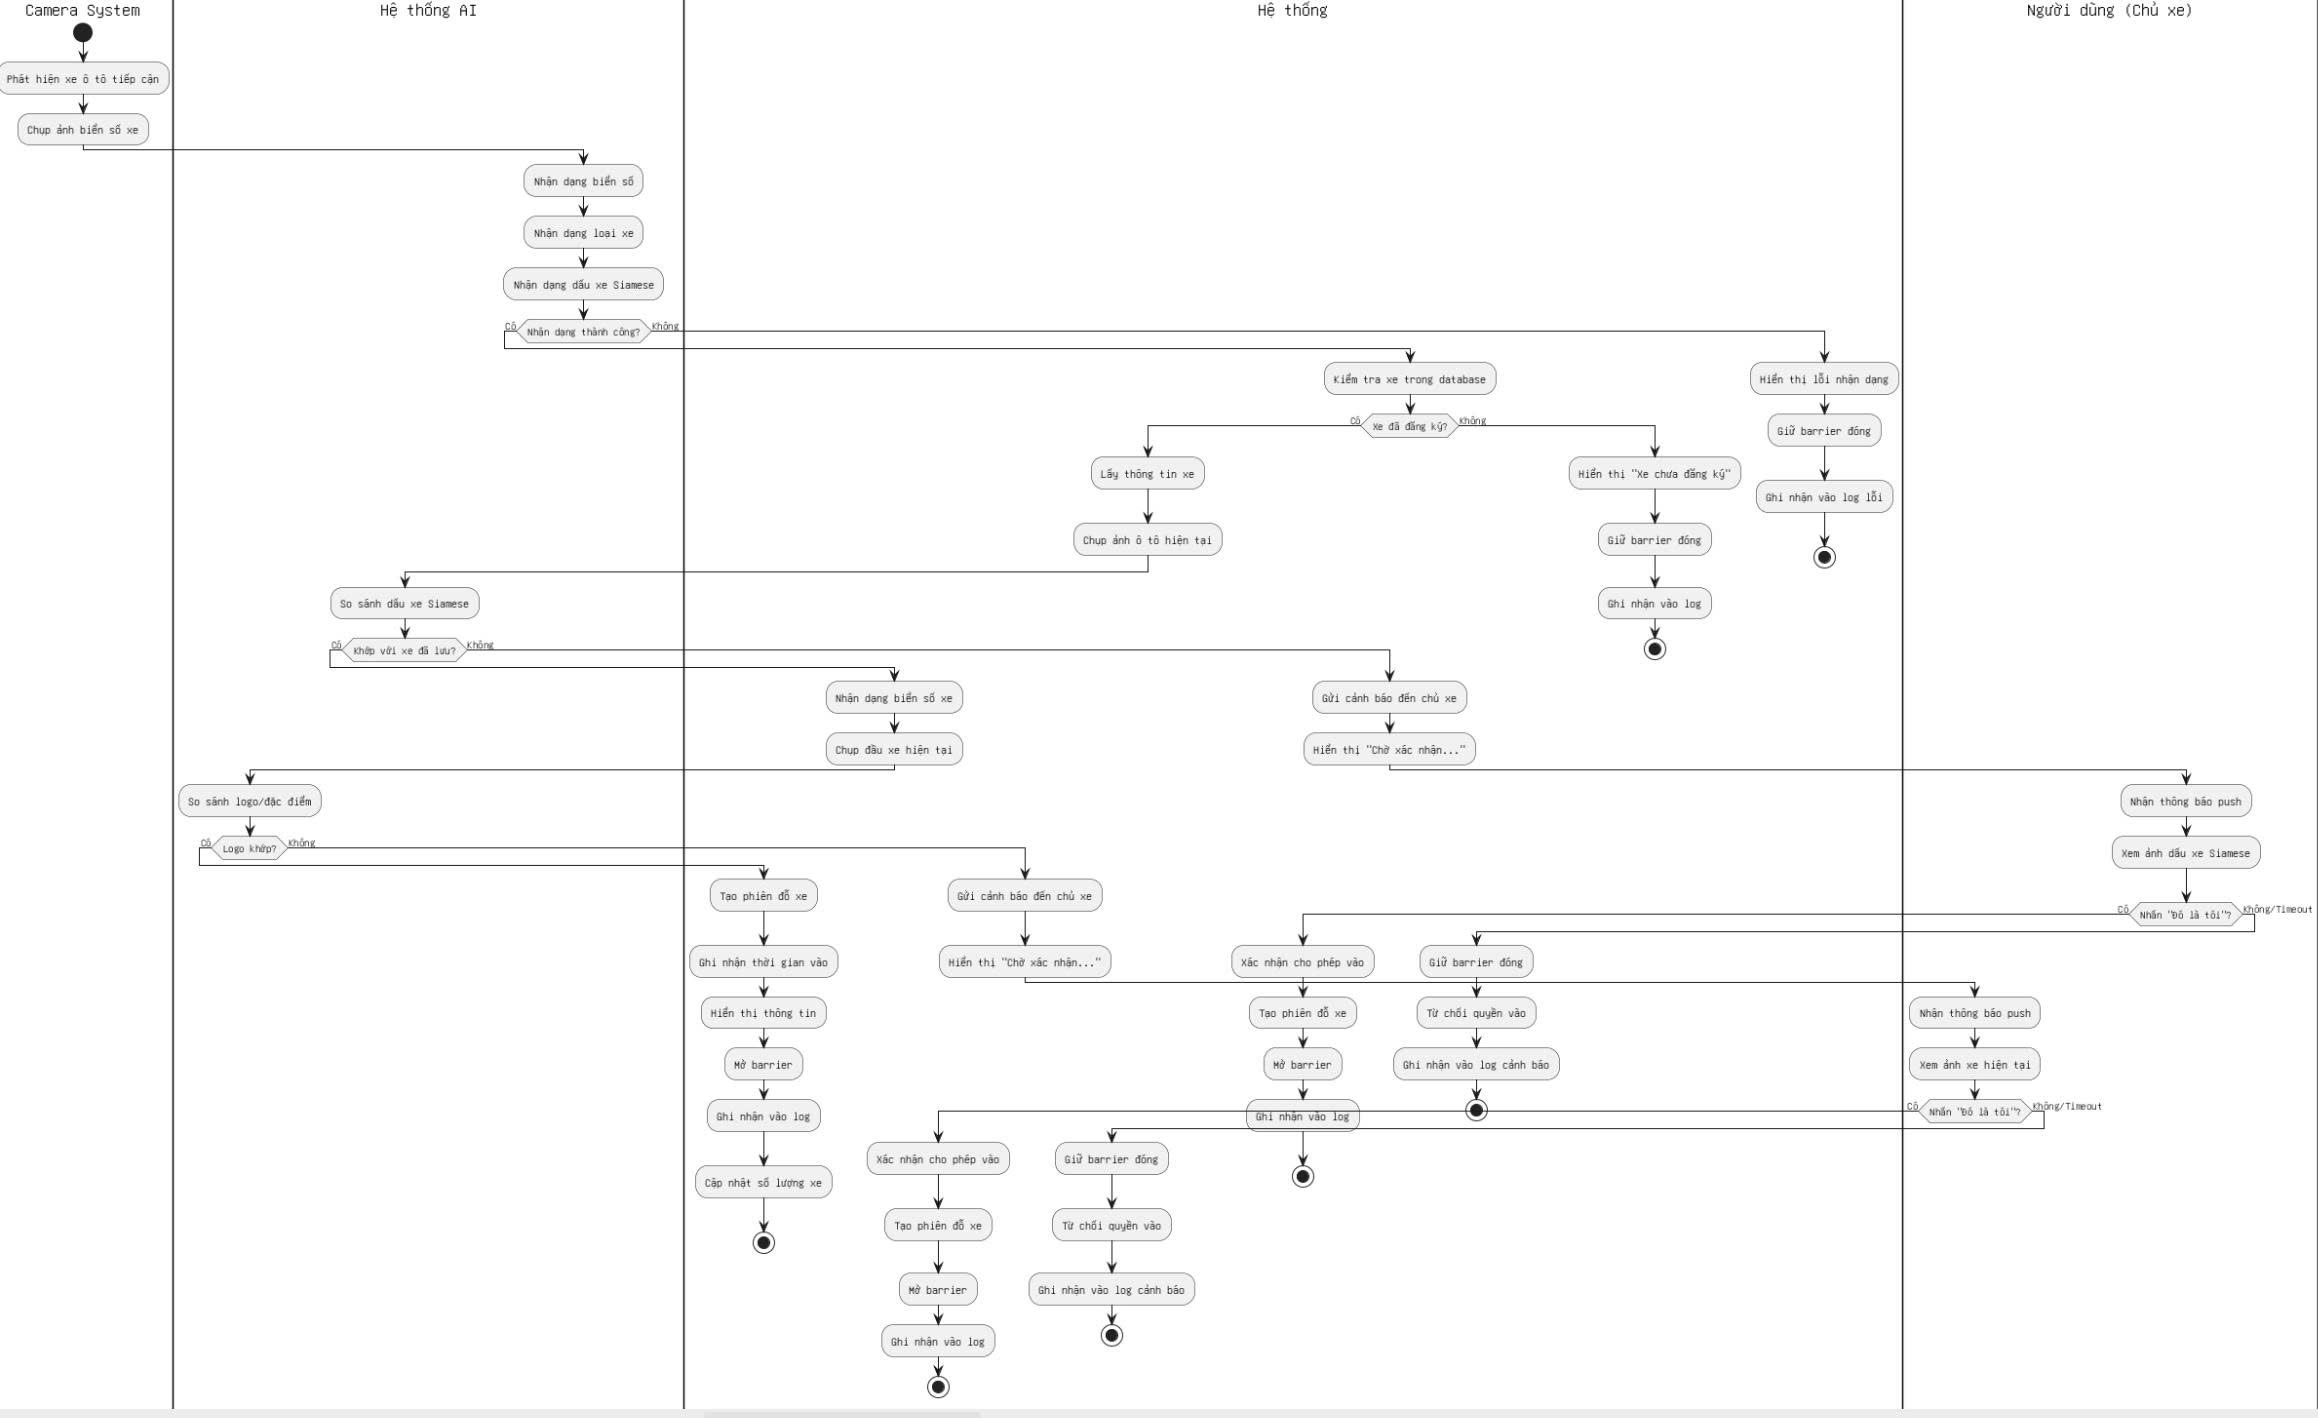
\includegraphics[width=1.0\textwidth]{figures/xeoto_vao.jpg}
    \caption{Sơ đồ Activity xử lý xe oto vào bãi đỗ}
    \label{fig:architecture}
\end{figure}

Mục đích: Activity diagram mô tả quy trình xử lý xe ô tô vào bãi đỗ, bao gồm nhận diện biển số xe, nhận diện logo xe, so sánh hình ảnh xe với cơ sở dữ liệu bằng Siamese Network và tạo phiên đỗ xe.

Quy trình bắt đầu khi camera phát hiện xe ô tô tiếp cận và chụp ảnh. Hệ thống AI tiến hành nhận dạng biển số, logo xe và trích xuất đặc trưng xe để phục vụ so sánh. Nếu nhận dạng thất bại hoặc xe chưa đăng ký trong hệ thống, hệ thống hiển thị lỗi, giữ barrier đóng và ghi nhận log.

Trong trường hợp xe đã đăng ký, hệ thống sử dụng Siamese Network để so sánh hình ảnh xe hiện tại với dữ liệu lưu trữ trong cơ sở dữ liệu. Nếu độ tương đồng vượt ngưỡng cho phép, hệ thống tạo phiên đỗ xe, mở barrier tự động và cập nhật thông tin xe vào hệ thống.

Nếu độ tương đồng không đạt ngưỡng, hệ thống tạo cảnh báo và gửi thông báo đến chủ xe để xác nhận. Dựa trên phản hồi của chủ xe hoặc khi hết thời gian chờ, hệ thống quyết định cho phép xe vào bãi hoặc từ chối, đồng thời ghi nhận log tương ứng. Quy trình kết thúc khi barrier được mở hoặc giữ đóng và dữ liệu được cập nhật.

\subsection{Sơ đồ Activity xử lý xe máy ra bãi đỗ}
\begin{figure}[H]
    \centering
    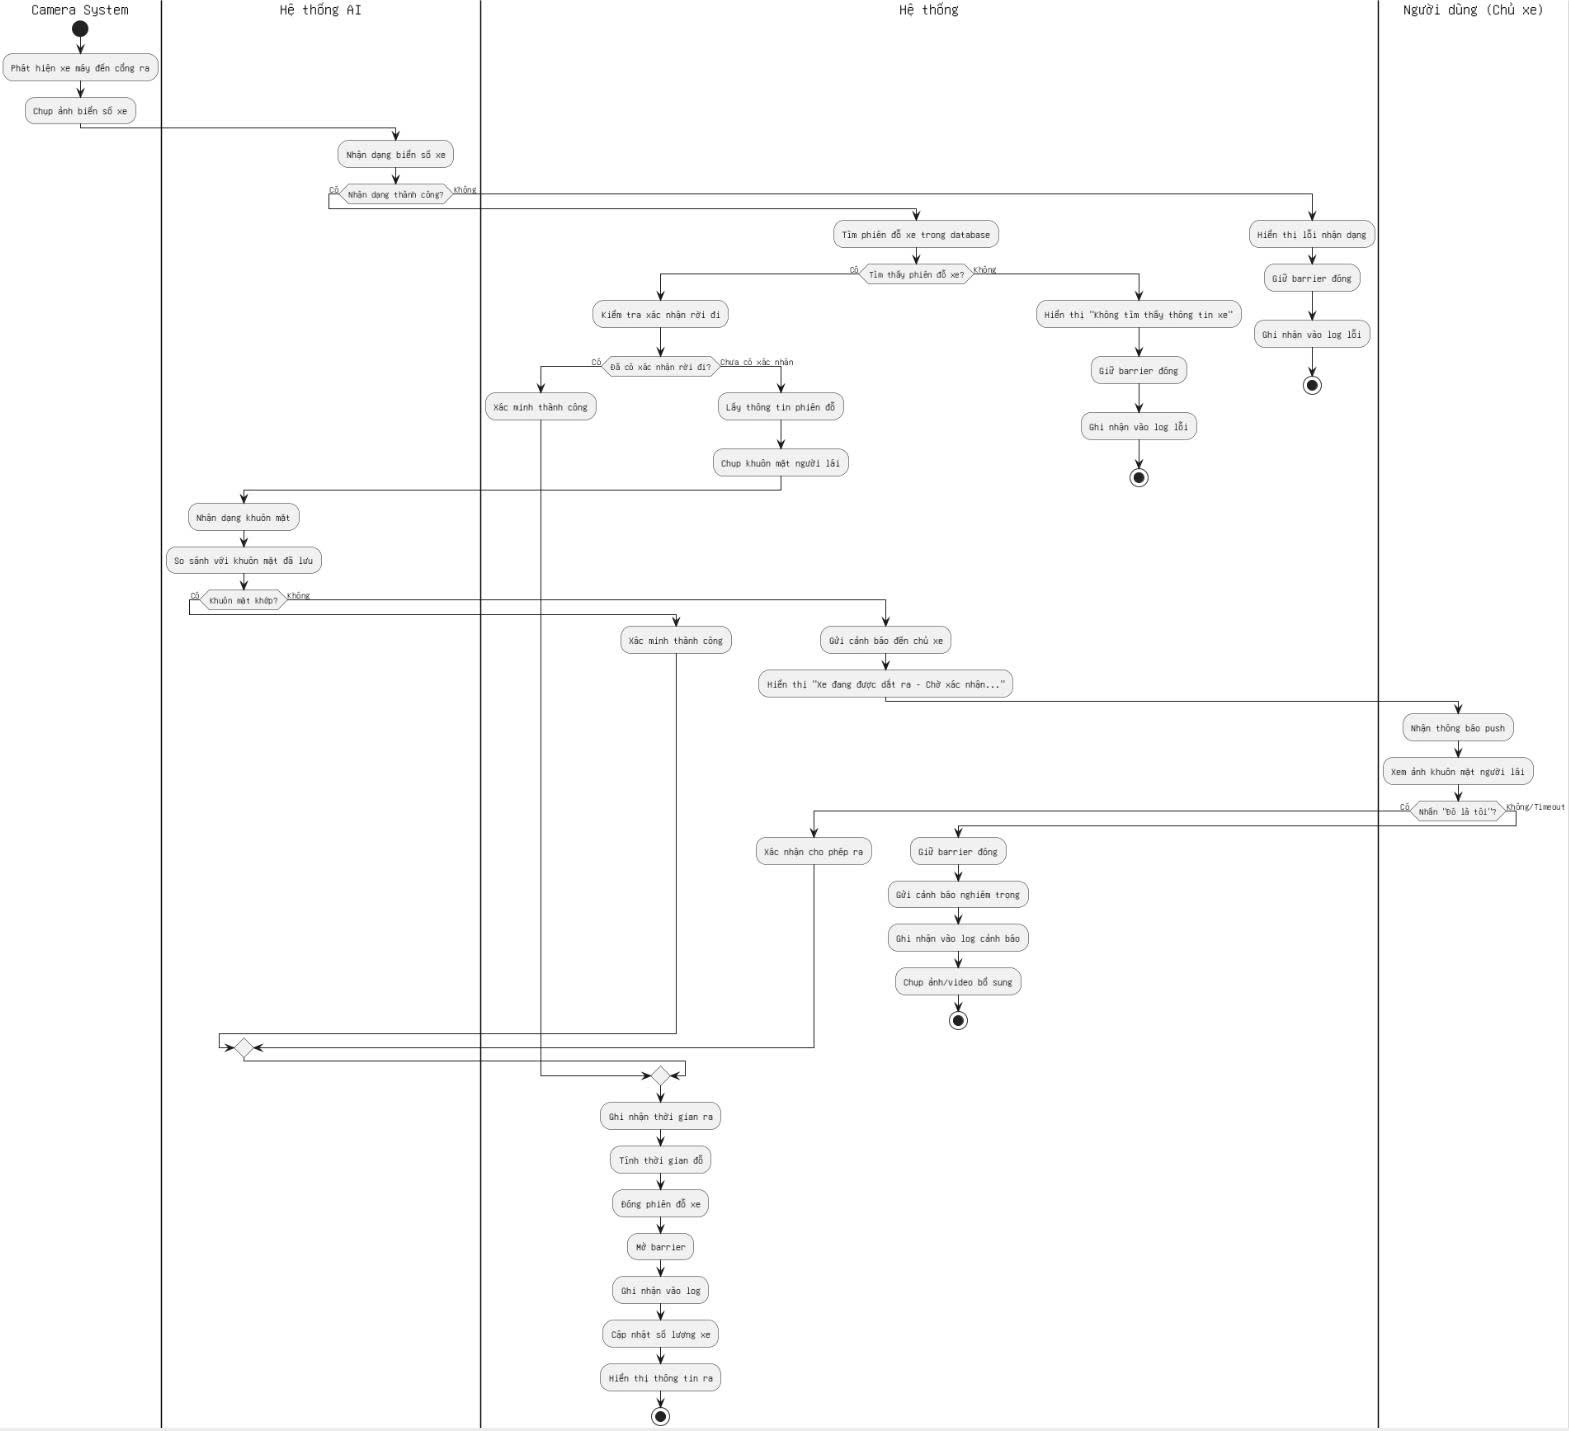
\includegraphics[width=0.95\textwidth]{figures/ac_xemay_ra.jpg}
    \caption{Sơ đồ Activity xử lý xe máy ra bãi đỗ}
    \label{fig:architecture}
\end{figure}


Mục đích: Activity diagram mô tả quy trình xử lý xe máy ra khỏi bãi đỗ, bao gồm nhận diện biển số xe, kiểm tra phiên đỗ xe, xác thực khuôn mặt người lái, kiểm tra xác nhận từ chủ xe.

Quy trình bắt đầu khi camera phát hiện xe máy đến cổng ra và chụp ảnh biển số xe. Hệ thống AI tiến hành nhận dạng biển số xe. Nếu nhận dạng thành công, hệ thống tìm phiên đỗ xe đang hoạt động trong database. Nếu nhận dạng thất bại hoặc không tìm thấy phiên đỗ xe, hệ thống hiển thị lỗi, giữ barrier đóng và ghi nhận log lỗi.

Khi tìm thấy phiên đỗ xe hợp lệ, hệ thống kiểm tra có xác nhận rời đi từ mobile app hay không. Nếu đã có xác nhận, hệ thống chụp khuôn mặt người lái và tiến hành so khớp với cơ sở dữ liệu. Nếu khuôn mặt khớp, hệ thống xác nhận thành công, lấy thông tin thời gian đỗ và chụp khuôn mặt người lái.

Nếu chưa có xác nhận từ mobile app, hệ thống hiển thị thông báo "Chưa có xác nhận từ chủ xe", tạo cảnh báo và gửi thông báo đến chủ xe. Người dùng nhận thông báo  và xác nhận. Dựa trên xác nhận của chủ xe "Người đó là tôi" , hệ thống quyết định cho phép xe ra hoặc giữ barrier đóng.

Quy trình kết thúc khi xe rời khỏi bãi đỗ và thông tin được hiển thị trống ra.
\subsection{Sơ đồ Activity xử lý xe oto ra bãi đỗ}
\begin{figure}[H]
    \centering
    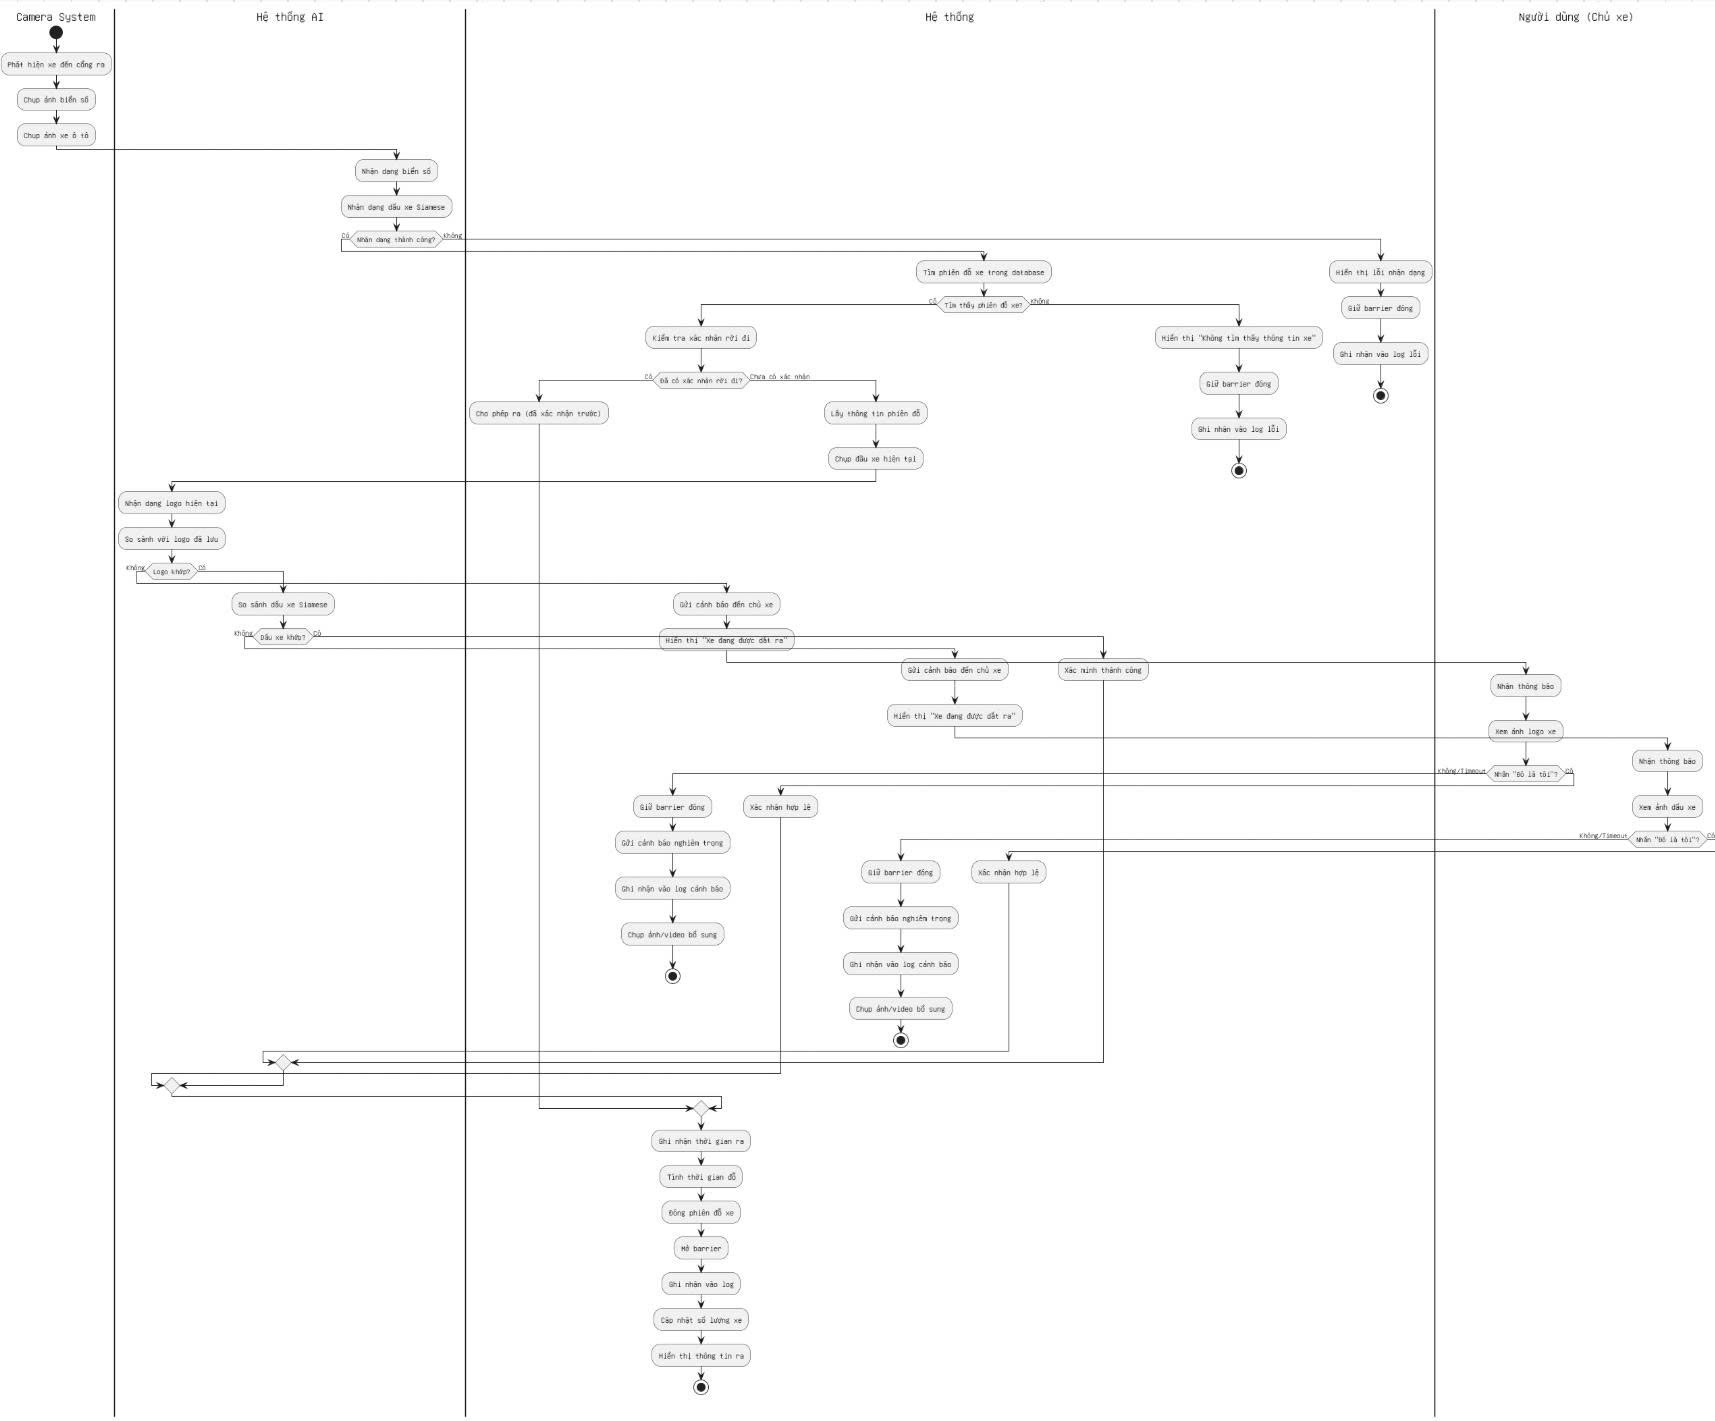
\includegraphics[width=0.95\textwidth]{figures/xeoto_ra.jpg}
    \caption{Sơ đồ Activity xử lý xe oto ra bãi đỗ}
    \label{fig:architecture}
\end{figure}



Mục đích: Activity diagram mô tả quy trình xử lý xe ô tô ra khỏi bãi đỗ, bao gồm nhận diện biển số xe, kiểm tra phiên đỗ xe, so sánh hình ảnh xe với Siamese Network, kiểm tra xác nhận từ chủ xe.

Quy trình bắt đầu khi camera phát hiện xe ô tô đến cổng ra và chụp ảnh biển số xe. Hệ thống AI tiến hành nhận dạng biển số xe. Nếu nhận dạng thành công, hệ thống tìm phiên đỗ xe đang hoạt động trong database. Nếu nhận dạng thất bại hoặc không tìm thấy phiên đỗ xe, hệ thống hiển thị lỗi "Không tìm thấy thông tin xe", giữ barrier đóng và ghi nhận log lỗi.

Khi tìm thấy phiên đỗ xe hợp lệ, hệ thống kiểm tra có xác nhận rời đi từ mobile app hay không. Nếu đã có xác nhận, hệ thống chụp ảnh xe hiện tại và lấy thông tin thời gian đỗ. Camera System ghi nhận khuôn mặt và tiến hành so sánh với khuôn mặt đã lưu sử dụng Siamese Network.

Nếu chưa có xác nhận từ mobile app, hệ thống hiển thị thông báo "Chờ đang được xét ra - Chờ xác nhận", gọi cảnh báo đến chủ xe và chờ phản hồi. Người dùng nhận thông báo báo gộp và xem ảnh đặc trưng xe Siamese. Dựa trên xác nhận "Người đó là tôi" của chủ xe hoặc khi hết timeout, hệ thống quyết định xác nhận cho phép ra hoặc giữ barrier đóng.

Sau khi xác thực thành công qua so sánh Siamese hoặc xác nhận của chủ xe. Hệ thống kết thúc phiên đỗ xe, cập nhật trạng thái trong database, mở barrier cho xe ra, ghi nhận vào log và cập nhật số lượng xe hiện tại trong bãi. Quy trình kết thúc khi xe rời khỏi bãi đỗ và thông tin trống ra được hiển thị.
\subsection{Sơ đồ Activity người dùng sử dụng app mobile }
\begin{figure}[H]
    \centering
    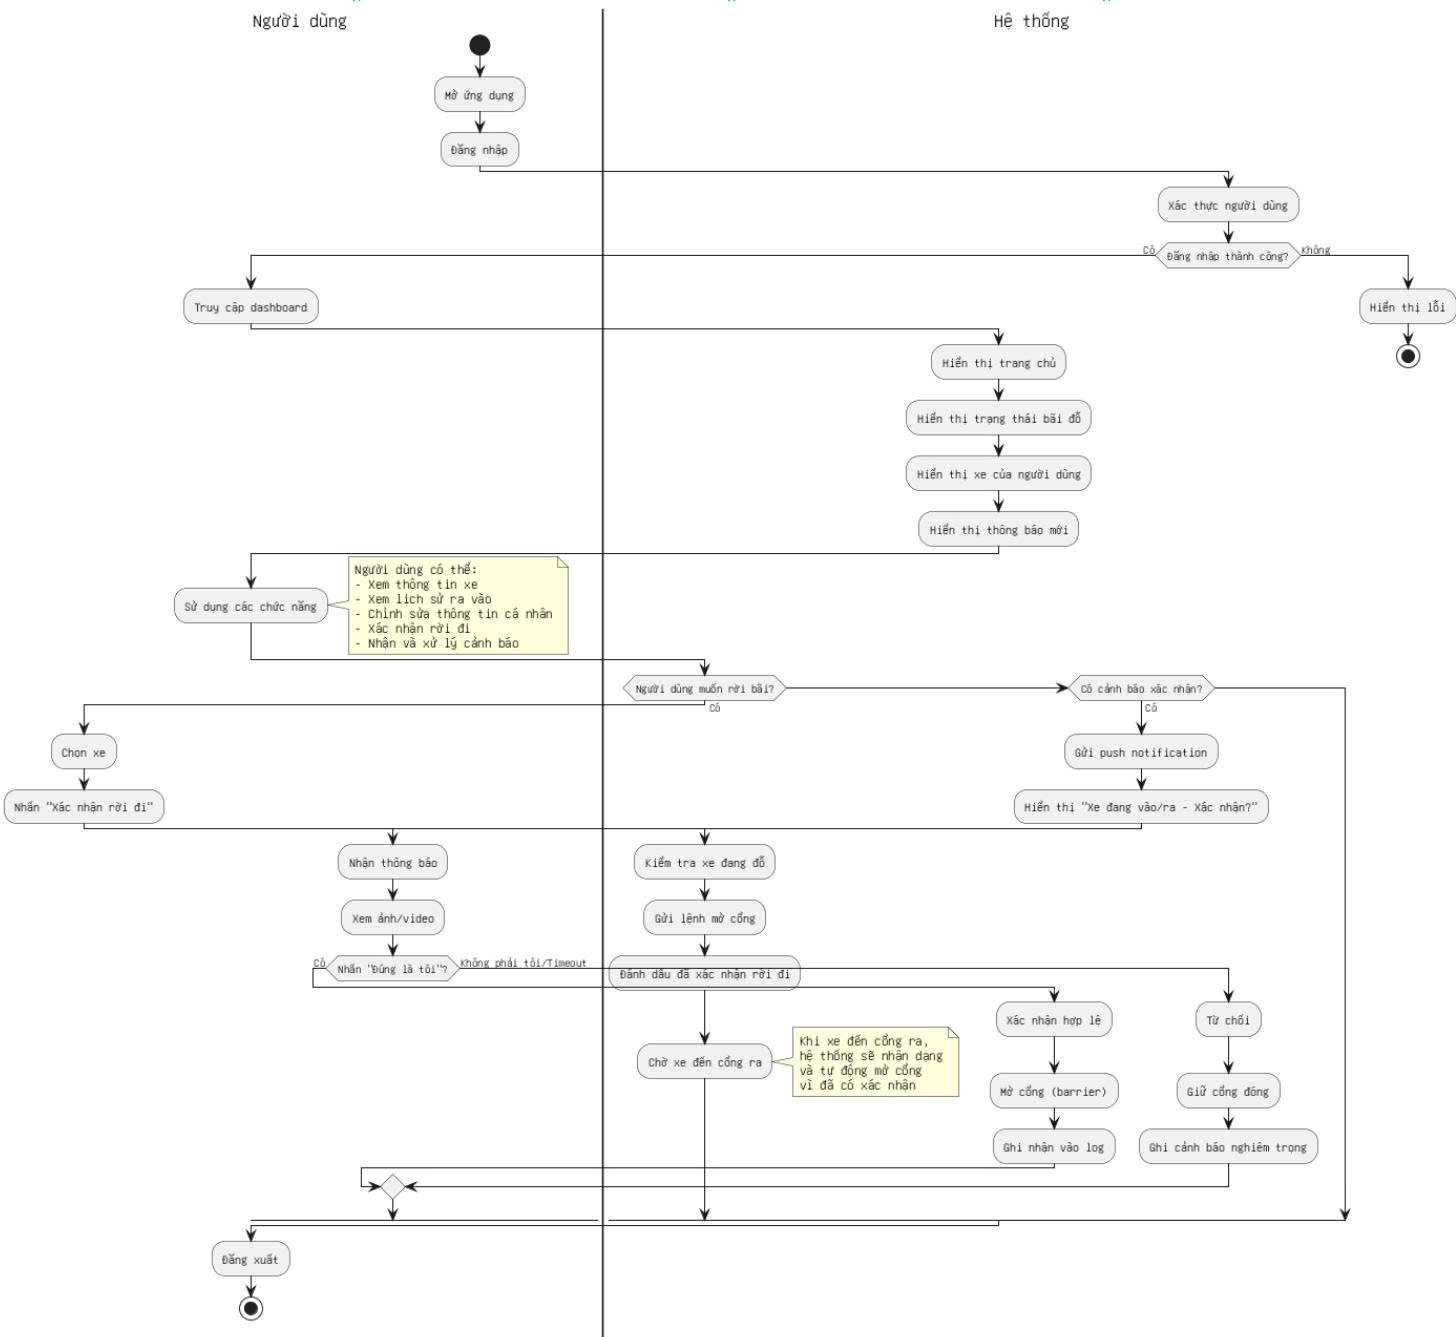
\includegraphics[width=0.95\textwidth]{figures/ac_user.jpg}
    \caption{Sơ đồ Activity người dùng sử dụng app mobile}
    \label{fig:architecture}
\end{figure}
Mục đích: Activity diagram mô tả quy trình người dùng tương tác với ứng dụng mobile để quản lý tài khoản, phương tiện, xác nhận rời bãi đỗ xe và nhận cảnh báo
\subsection{Sơ đồ Activity bảo vệ sử dụng app mobile }
\begin{figure}[H]
    \centering
    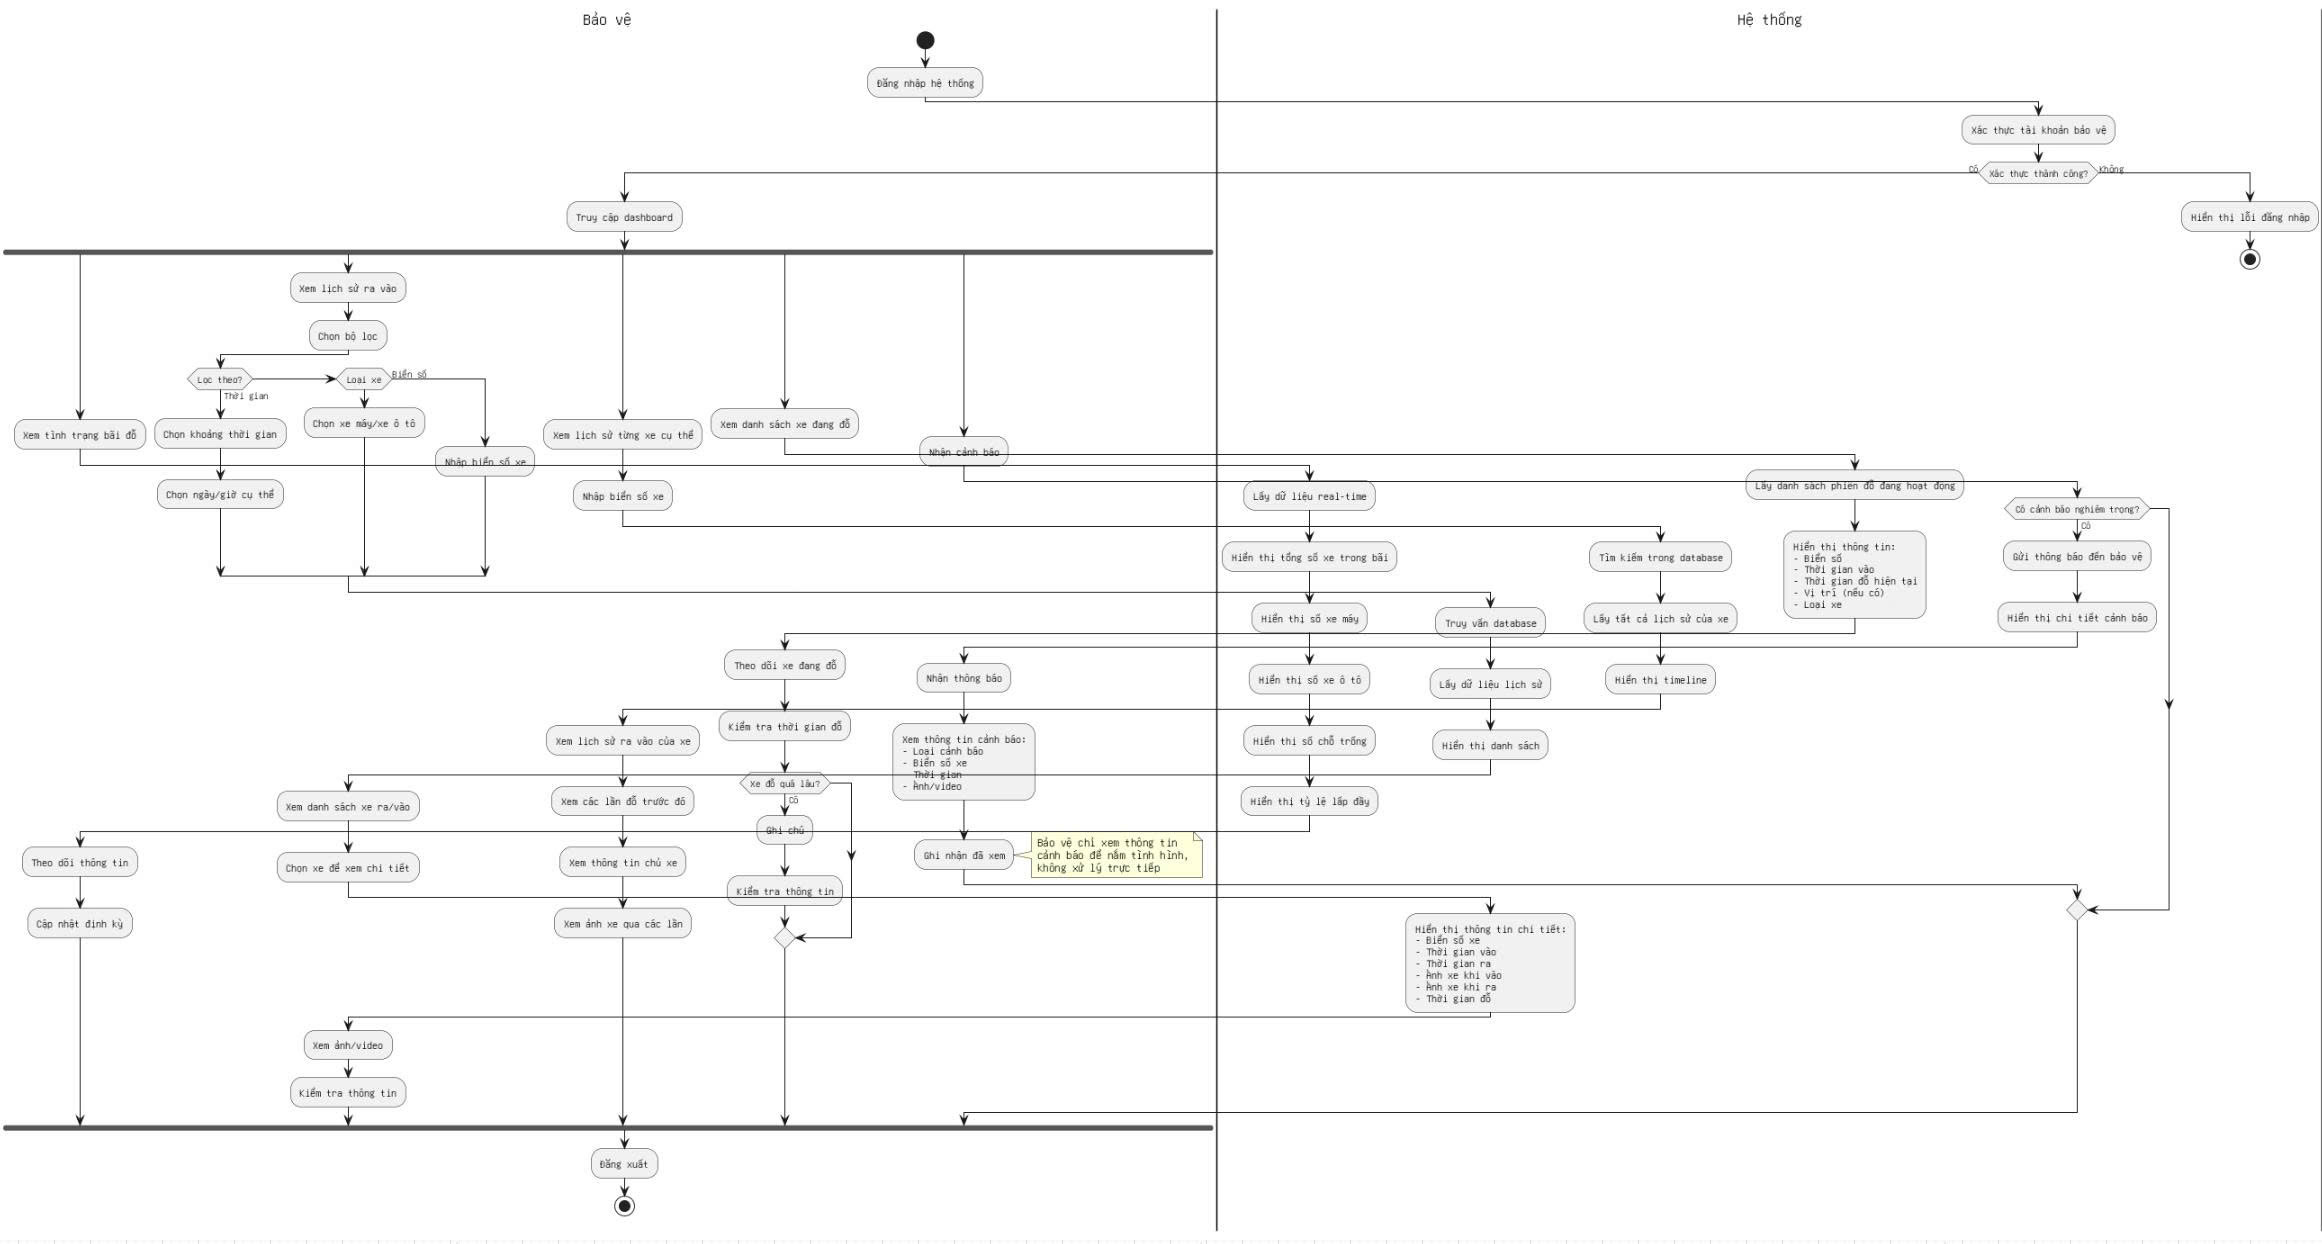
\includegraphics[width=0.95\textwidth]{figures/ac_baove.jpg}
    \caption{Sơ đồ Activity bảo vệ sử dụng app mobile }
    \label{fig:architecture}
\end{figure}
Mục đích: Activity diagram mô tả quy trình nhân viên bảo vệ sử dụng ứng dụng mobile để đăng nhập, giám sát xe trong bãi, xem lịch sử ra vào và xử lý cảnh báo.
\section{Sơ đồ lớp}
\begin{figure}[H]
    \centering
    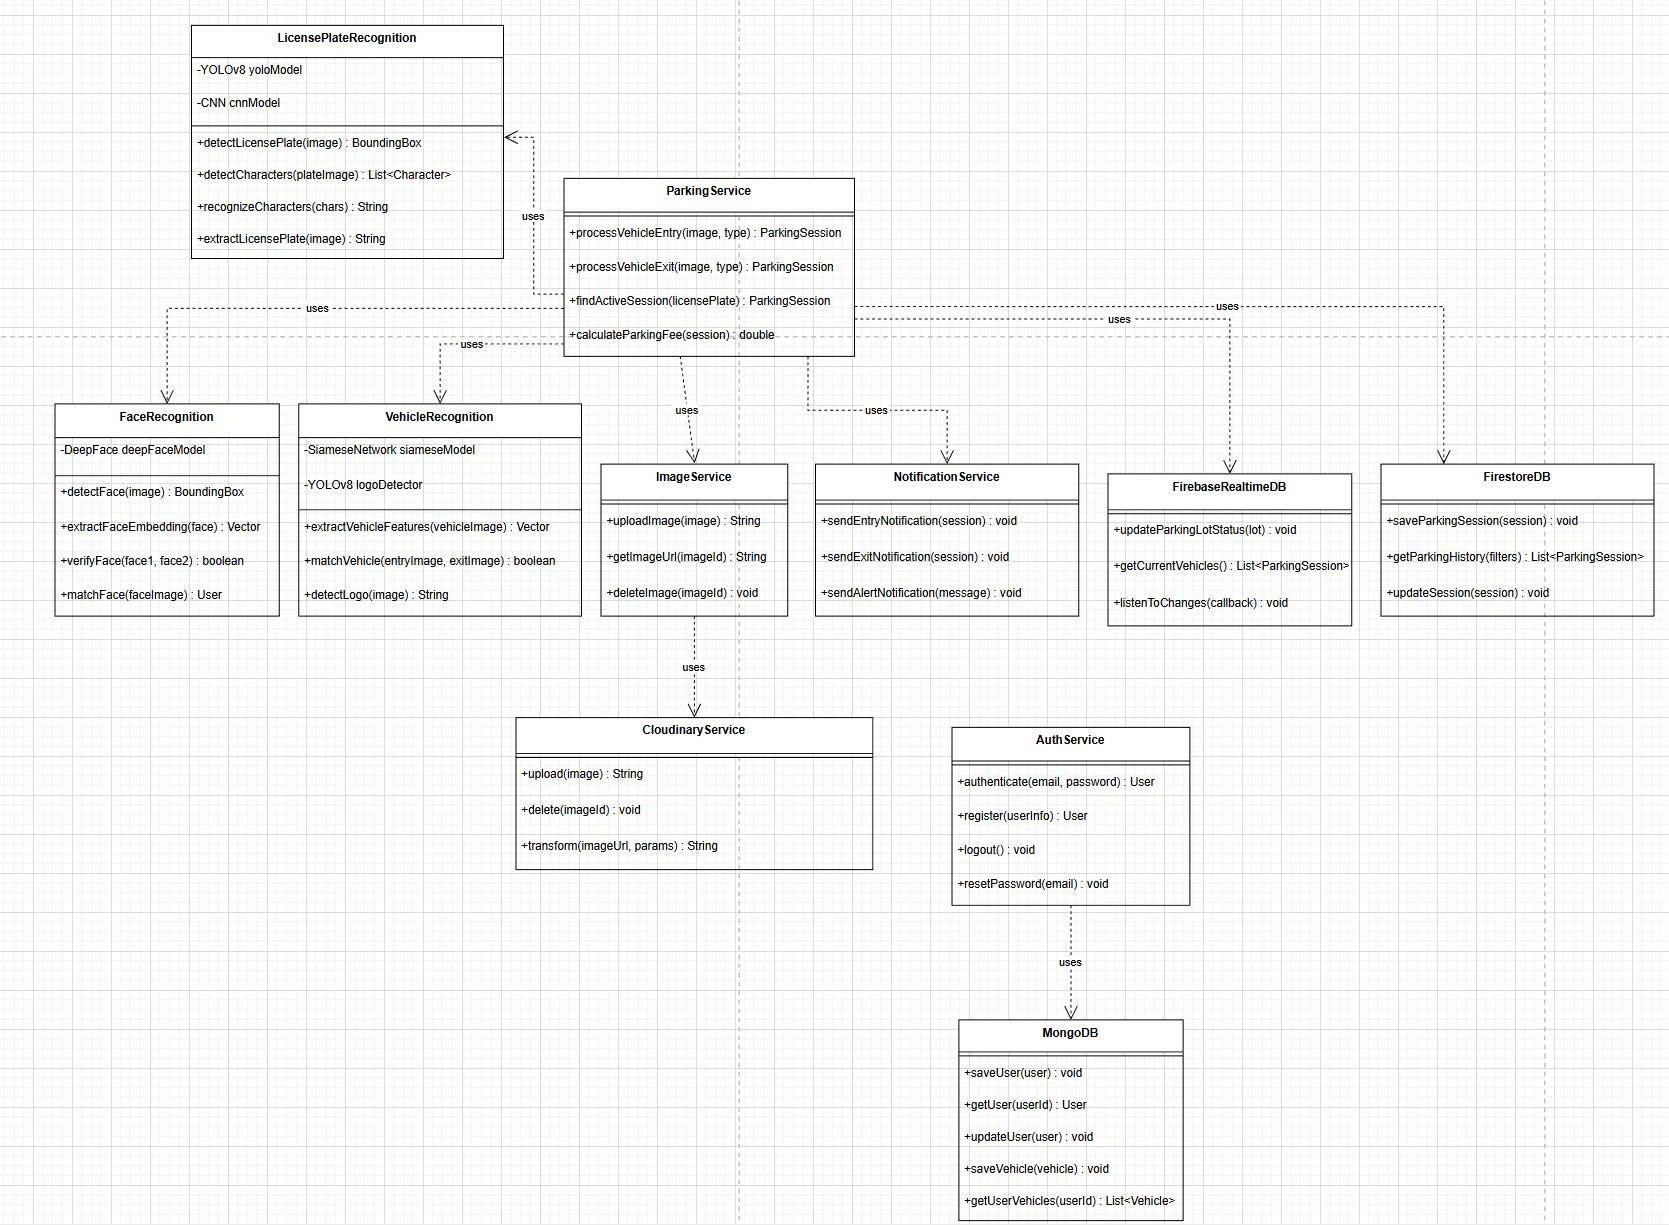
\includegraphics[width=0.85\textwidth]{figures/lop_tq.jpg}
    \caption{Sơ đồ lớp hệ thống quản lý bãi đỗ xe thông minh}
    \label{fig:architecture}
\end{figure}


\subsection{Nhóm AI/Computer Vision}
\subsubsection{License Plate Recognition}

Lớp chịu trách nhiệm nhận diện biển số xe sử dụng hai mô hình AI:
\begin{itemize}
    \item YOLOv8 yoloModel: Phát hiện vị trí biển số trong ảnh
    \item CNN cnnModel: Nhận diện ký tự trên biển số
\end{itemize}
Cung cấp các phương thức:
\begin{itemize}
    \item detectLicensePlate(): Tìm vùng chứa biển số
    \item detectCharacters(): Nhận diện từng ký tự
    \item recognizeCharacters(): Chuyển đổi ký tự thành chuỗi
    \item extractLicensePlate(): Trích xuất kết quả cuối cùng
\end{itemize}

\subsubsection{Face Recognition}
Lớp xác thực khuôn mặt người dùng sử dụng:
\begin{itemize}
    \item DeepFace deepFaceModel: Mô hình nhận diện khuôn mặt
\end{itemize}
Các chức năng chính:
\begin{itemize}
    \item detectFace(): Phát hiện khuôn mặt trong ảnh
    \item extractFaceEmbedding(): Trích xuất đặc trưng khuôn mặt
    \item verifyFace(): So sánh hai khuôn mặt
    \item matchFace(): Tìm khuôn mặt khớp trong cơ sở dữ liệu
\end{itemize}

\subsubsection{Vehicle Recognition}
Lớp nhận diện loại xe:
\begin{itemize}
    \item SiameseNetwork siameseModel: Mạng Siamese để phân loại
    \item YOLOv8 logoDetector: Phát hiện logo xe
\end{itemize}
Phương thức:
\begin{itemize}
    \item extractVehicleFeatures(): Trích xuất đặc trưng xe
    \item matchVehicle(): Khớp với xe trong database
    \item detectLogo(): Nhận diện thương hiệu xe
\end{itemize}

\subsection{Nhóm Service Layer}

Lớp nghiệp vụ chính xử lý logic bãi đỗ xe:
\begin{itemize}
    \item processVehicleEntry(): Xử lý xe vào 
    \item processVehicleExit(): Xử lý xe ra 
    \item findActiveSession(): Tìm phiên đỗ xe đang hoạt động
\end{itemize}

\subsubsection{Image Service}
Quản lý xử lý và lưu trữ ảnh:
\begin{itemize}
    \item uploadImage(): Upload ảnh lên cloud storage
    \item getImageUrl(): Lấy URL ảnh đã lưu
    \item deleteImage(): Xóa ảnh không cần thiết
\end{itemize}

\subsubsection{Notification Service}
Gửi thông báo cho người dùng:
\begin{itemize}
    \item sendEntryNotification(): Thông báo xe vào bãi
    \item sendExitNotification(): Thông báo xe ra 
    \item sendAlertNotification(): Cảnh báo bất thường
\end{itemize}

\subsubsection{Cloudinary Service}
Tích hợp với Cloudinary để lưu trữ ảnh:
\begin{itemize}
    \item upload(): Upload ảnh
    \item delete(): Xóa ảnh
    \item transform(): Chỉnh sửa/tối ưu ảnh
\end{itemize}

\subsubsection{Auth Service}
Xác thực và quản lý người dùng:
\begin{itemize}
    \item authenticate(): Xác thực email/password
    \item register(): Đăng ký tài khoản mới
    \item logout(): Đăng xuất
    \item resetPassword(): Đặt lại mật khẩu
\end{itemize}

\subsection{Nhóm Database}

\subsubsection{Firebase Realtime DB}
Lưu trữ real-time:
\begin{itemize}
    \item updateParkingLotStatus(): Cập nhật trạng thái bãi đỗ
    \item getCurrentVehicles(): Lấy danh sách xe hiện tại
    \item listenToChanges(): Lắng nghe thay đổi real-time
\end{itemize}

\subsubsection{Firestore DB}
Lưu trữ dữ liệu cấu trúc:
\begin{itemize}
    \item saveParkingSession(): Lưu phiên đỗ xe
    \item getParkingHistory(): Lấy lịch sử đỗ xe
    \item updateSession(): Cập nhật thông tin phiên
\end{itemize}

\subsubsection{MongoDB}
Lưu trữ thông tin người dùng:
\begin{itemize}
    \item saveUser(): Lưu thông tin user
    \item getUser(): Lấy thông tin user
    \item updateUser(): Cập nhật user
    \item saveVehicle(): Lưu thông tin xe
    \item getUserVehicles(): Lấy danh sách xe của user
\end{itemize}

\subsection{Luồng Hoạt Động}

\begin{itemize}
    

    \item \textbf{Xe vào}: Camera chụp $\rightarrow$ LicensePlateRecognition (YOLO + CNN) $\rightarrow$ VehicleRecognition $\rightarrow$ ParkingService.processVehicleEntry() $\rightarrow$ ImageService.uploadImage() $\rightarrow$ FirestoreDB.saveParkingSession() + FirebaseRealtimeDB $\rightarrow$ NotificationService.sendEntryNotification()
    
    \item \textbf{Xe ra}: Camera chụp $\rightarrow$ LicensePlateRecognition $\rightarrow$ ParkingService.findActiveSession() $\rightarrow$ ParkingService.calculateParkingFee() $\rightarrow$ FirestoreDB.updateSession() $\rightarrow$ NotificationService.sendExitNotification()
    
    \item \textbf{Xác thực}: FaceRecognition.detectFace() $\rightarrow$ FaceRecognition.verifyFace() $\rightarrow$ AuthService.authenticate() $\rightarrow$ MongoDB.getUser() $\rightarrow$ Cấp quyền truy cập
    
    \item \textbf{Quản lý ảnh}: ImageService $\rightarrow$ Cloudinary.uploadImage() $\rightarrow$ Cloudinary.transformImage() $\rightarrow$ Trả về URL

\end{itemize}
\section{Thiết kế CSDL}
% \subsection{Thiết kế cơ sở dữ liệu}

Hệ thống sử dụng mô hình cơ sở dữ liệu NoSQL nhằm đáp ứng yêu cầu lưu trữ dữ liệu phi cấu trúc, mở rộng linh hoạt và xử lý thời gian thực. Cụ thể, hệ thống kết hợp ba công nghệ: MongoDB, Firebase Firestore và Firebase Realtime Database, trong đó mỗi loại đảm nhiệm một vai trò khác nhau.
\subsection{MongoDB – Quản lý thông tin người dùng và phương tiện}

MongoDB được sử dụng để lưu trữ thông tin người dùng và phương tiện do có cấu trúc dữ liệu rõ ràng, ổn định và phù hợp với các thao tác truy vấn phức tạp. Collection \texttt{User} bao gồm các thông tin như tài khoản người dùng, danh sách phương tiện đăng ký  và các thông tin liên quan khác. 

\subsection{Firestore – Lưu trữ lịch sử hoạt động}

Firebase Firestore được sử dụng để lưu trữ lịch sử hoạt động của hệ thống do khả năng mở rộng tốt và hỗ trợ cấu trúc dữ liệu phân cấp. Dữ liệu lịch sử được tổ chức theo dạng nhiều collection con như sau:

\begin{itemize}
    \item lichsuhoatdong (collection)
    \item Ngày hoạt động (document)
    \item xemay / xeoto (collection)
    \item Biển số xe (document)
    \item timeline (collection)
\end{itemize}

Mỗi document trong collection timeline lưu trữ một lần ra/vào của phương tiện, bao gồm các trường dữ liệu như biển số xe vào/ra, thời gian vào/ra, hình ảnh khuôn mặt và các thông tin xác thực liên quan. Ngoài ra, hệ thống còn lưu số lần ra/vào thông qua các trường solanvao và solanra để phục vụ thống kê và giám sát.

\subsection{Realtime Database – Quản lý trạng thái xe trong bãi}

Firebase Realtime Database được sử dụng để lưu trữ danh sách biển số xe đang có mặt trong bãi đỗ. Cơ sở dữ liệu này hỗ trợ cập nhật và đồng bộ dữ liệu theo thời gian thực, cho phép hệ thống nhanh chóng xác định trạng thái hiện tại của phương tiện (đang trong bãi hoặc đã rời đi), từ đó phục vụ cho việc kiểm soát ra vào và hiển thị thông tin tức thời trên giao diện quản lý.




\section{Thiết kế giao diện}
\subsection{Giao diện chính destop app }
\begin{figure}[H]
    \centering
    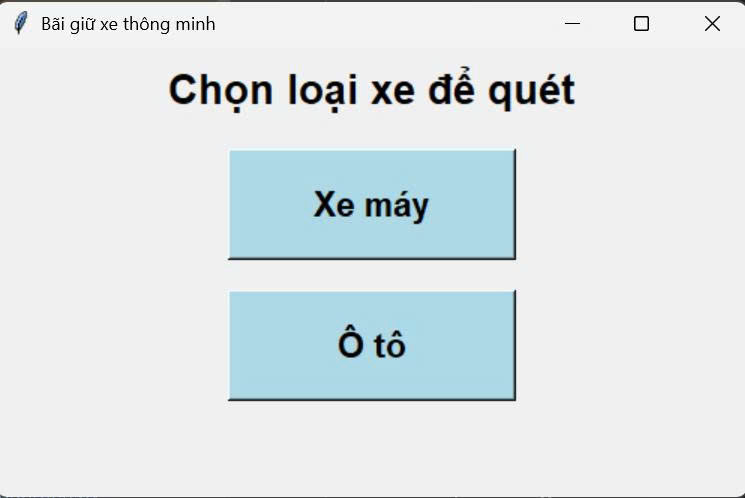
\includegraphics[width=0.5\textwidth]{figures/giaodienchinh.jpg}
    \caption{Giao diện chính desktop app }
    \label{fig:architecture}
\end{figure}
\subsection{Giao diện xử lý xe máy ra vào bãi đỗ}
\begin{figure}[H]
    \centering
    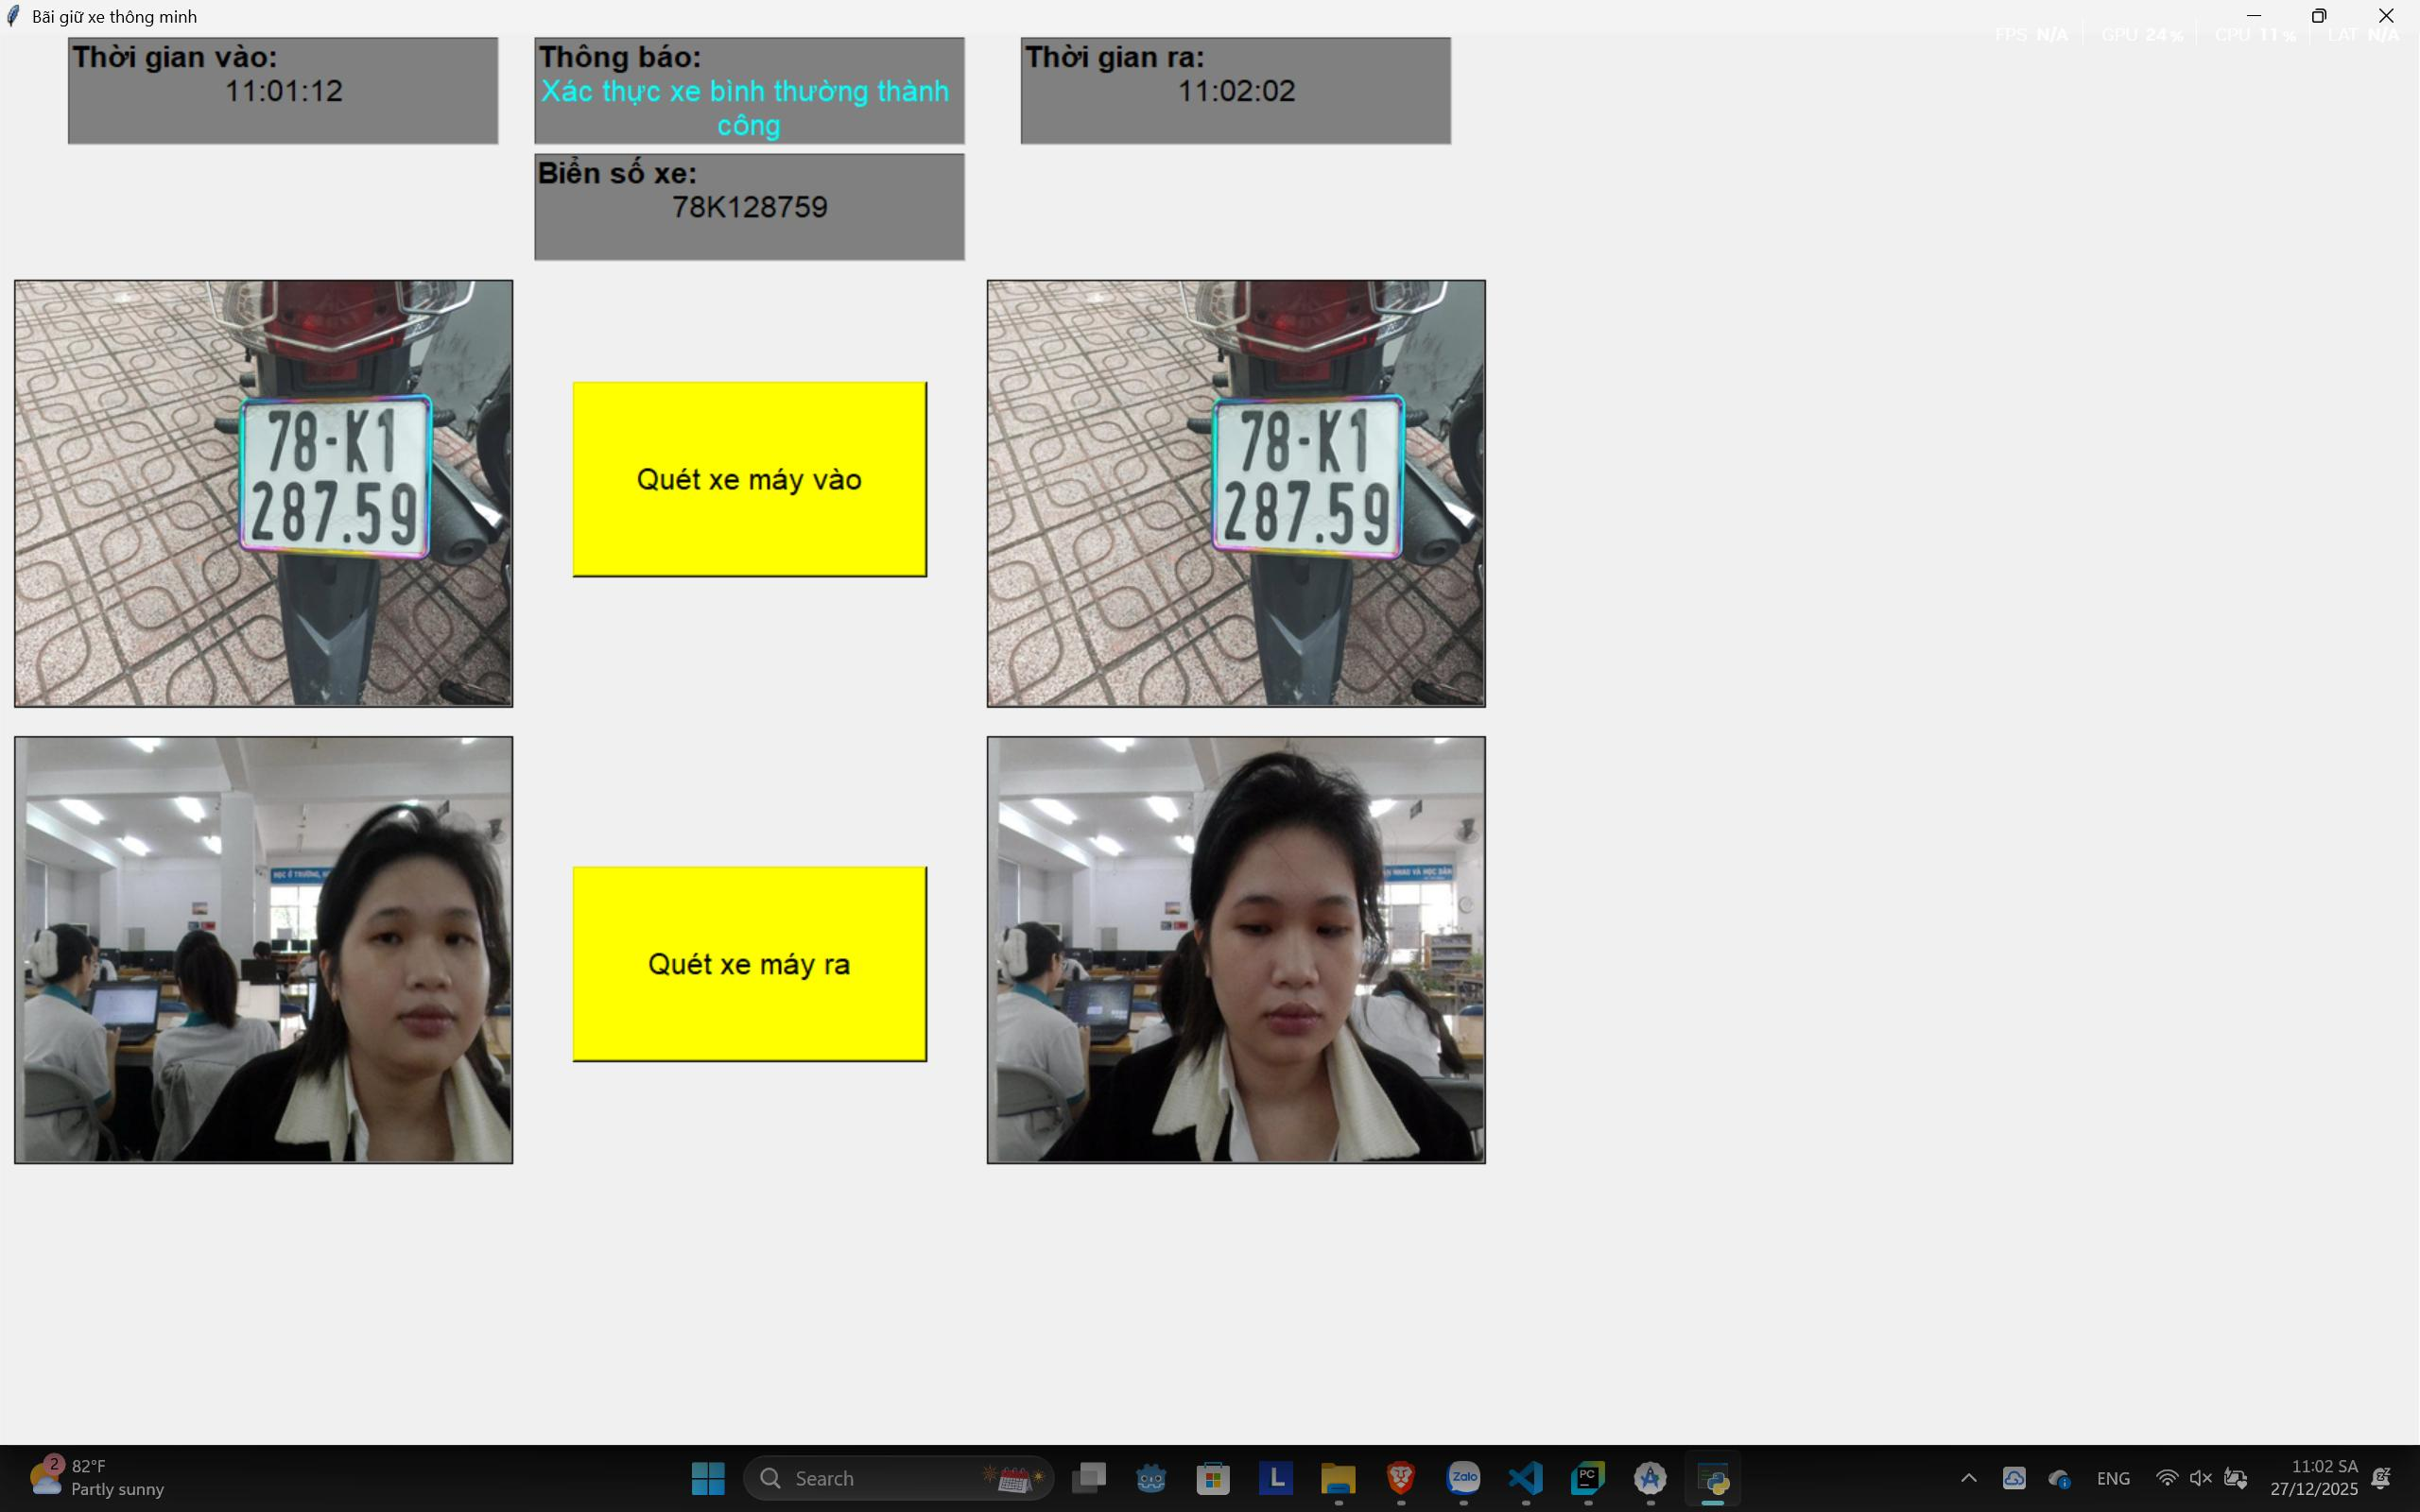
\includegraphics[width=0.85\textwidth]{figures/giaodien_xemay.jpg}
    \caption{Giao diện xử lý xe máy ra vào bãi đỗ}
    \label{fig:parking_interface}
\end{figure}
Hình \ref{fig:parking_interface} mô tả giao diện quét xe máy của hệ thống. Giao diện hiển thị thông tin: thời gian vào , biển số xe , thời gian ra. Bên trái là ảnh xe máy và khuôn mặt khi vào, bên phải là ảnh xe máy và khuôn mặt khi ra, kèm trạng thái xác thực "Quét xe máy vào" và "Quét xe máy ra".
\subsection{Giao diện xử lý xe ô tô ra vào bãi đỗ}
\begin{figure}[H]
    \centering
    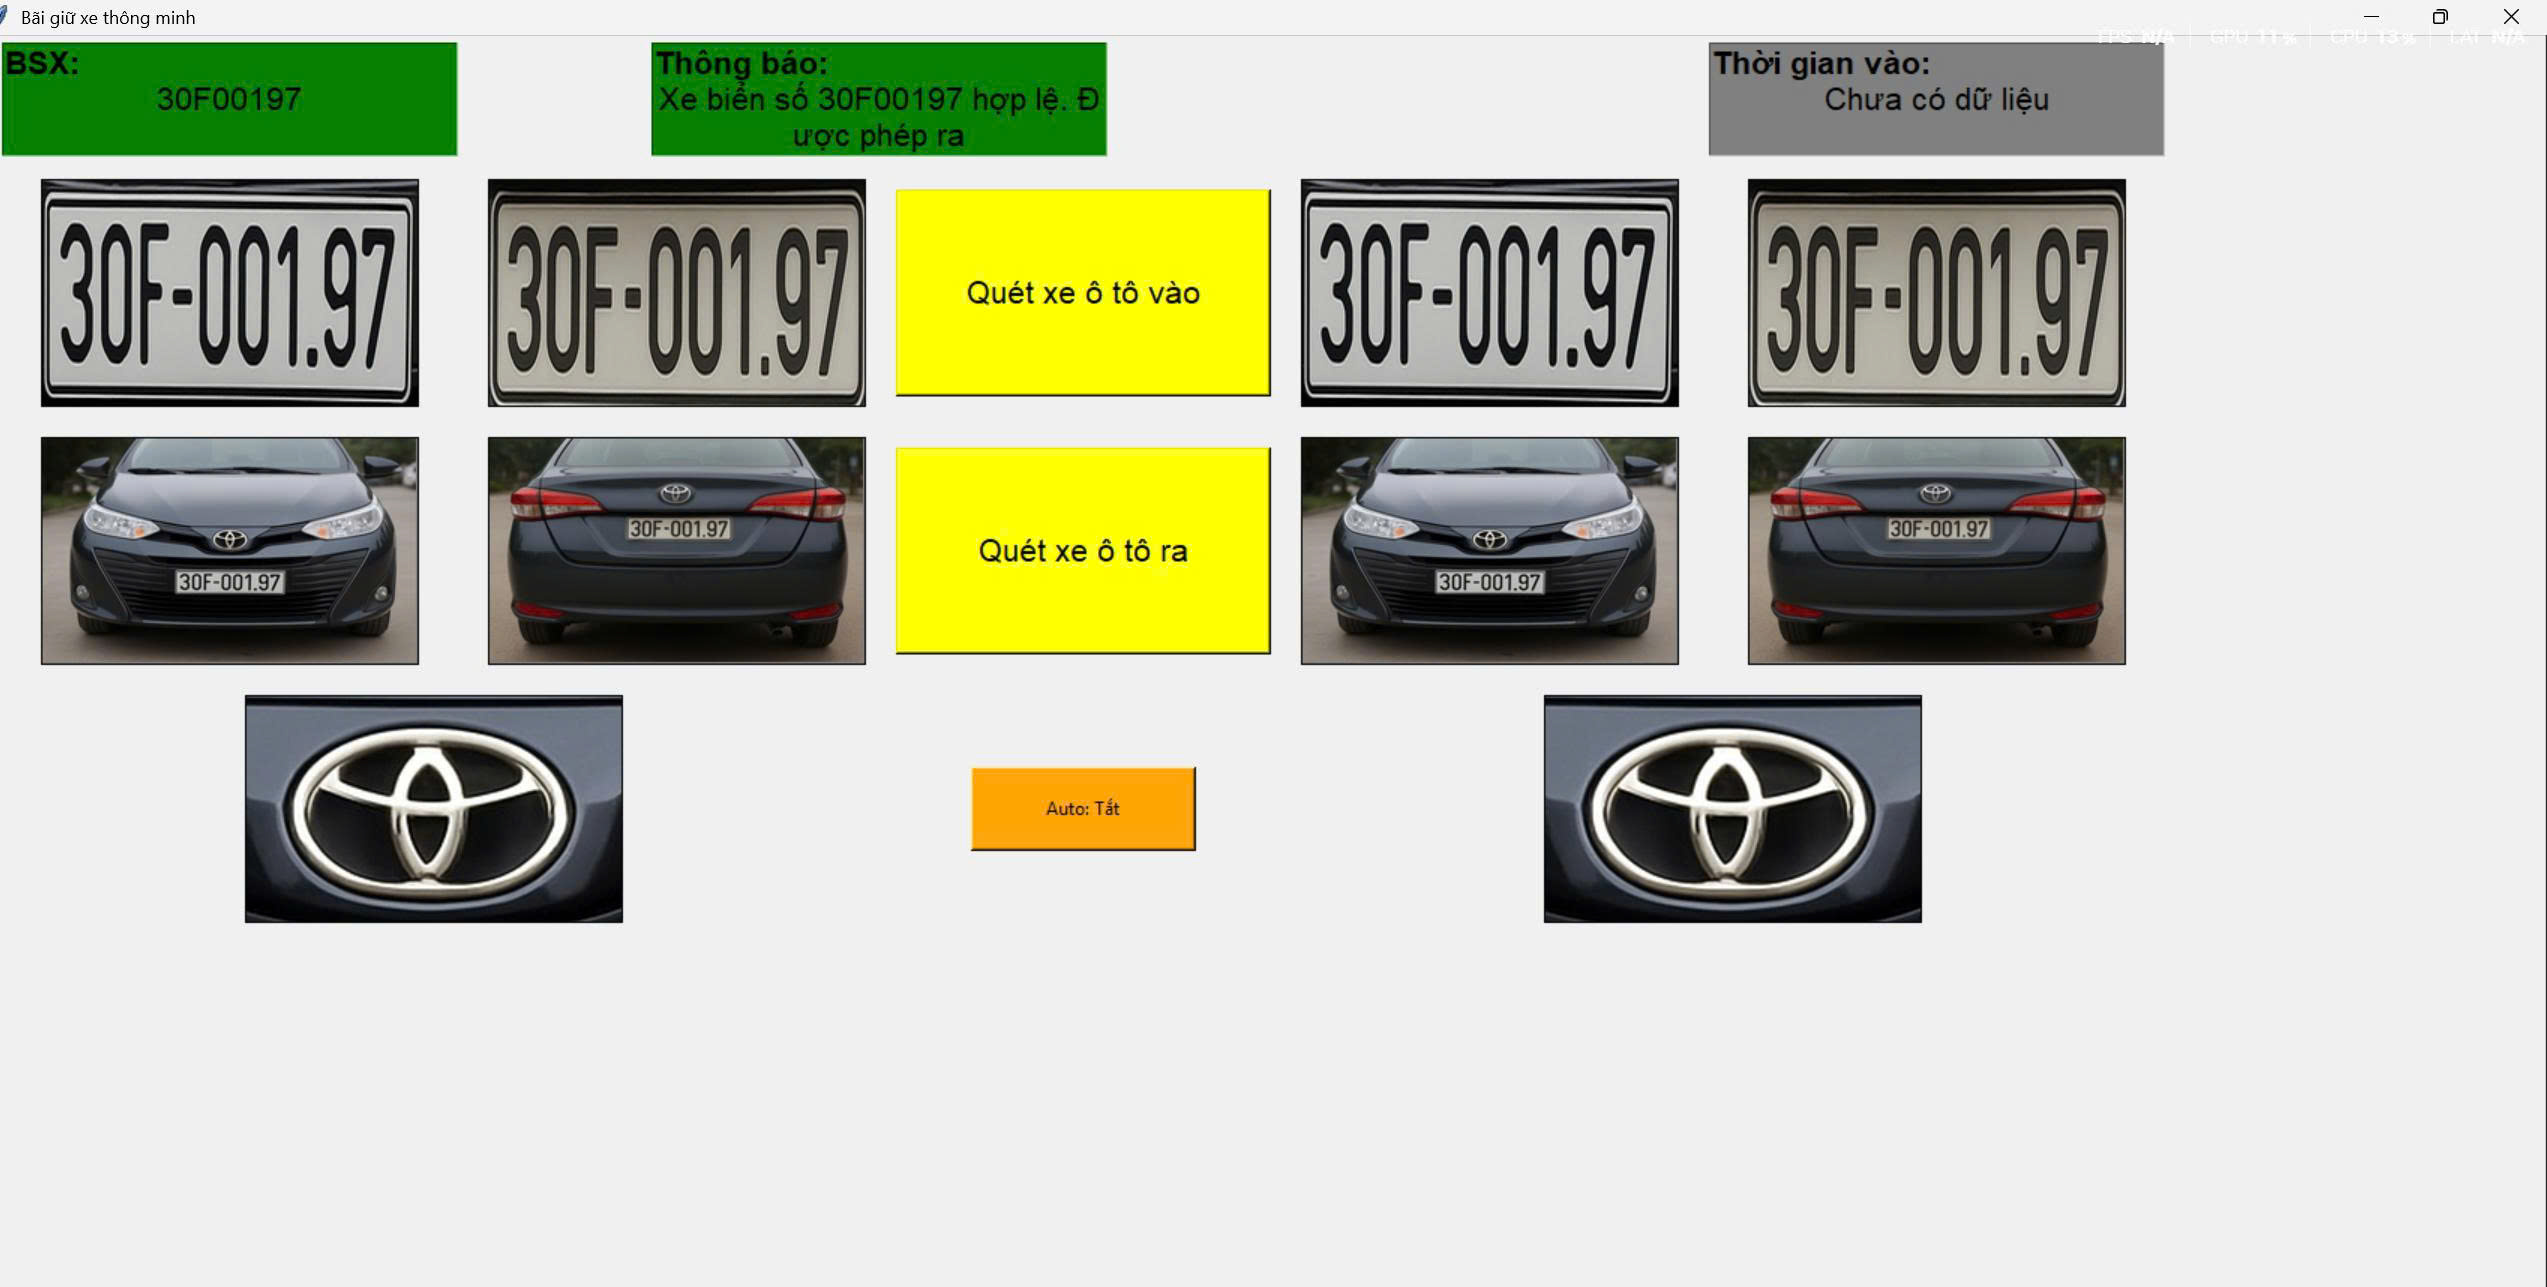
\includegraphics[width=0.8\textwidth]{figures/giaodien_oto.jpg}
    \caption{Giao diện xử lý xe ô tô ra vào bãi đỗ}
    \label{fig:car_parking}
\end{figure}
Hình \ref{fig:car_parking} thể hiện giao diện quét xe ô tô. Hệ thống hiển thị biển số xe và thông báo xe hợp lệ được phép ra. Bên trái là hình ảnh xe vào (biển số, mặt trước và logo), bên phải là hình ảnh xe ra (biển số, mặt sau và logo). Hệ thống sử dụng mạng Siamese để so sánh đặt trừng của đầu xe và so sánh logo xe lúc ra vào.
\subsection{Giao diện mobile app đăng ký}
\begin{figure}[H]
    \centering      
    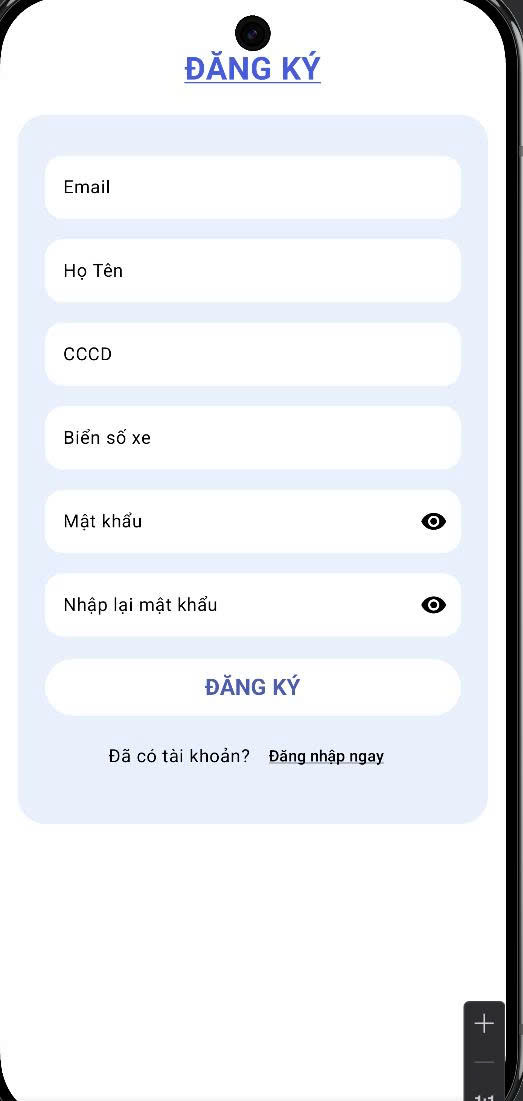
\includegraphics[width=0.5\textwidth]{figures/mh_dk.jpg}
    \caption{Giao diện mobile app đăng ký}
    \label{fig:register}
\end{figure}
Hình \ref{fig:register} hiển thị giao diện đăng ký với các trường thông tin: Email, Họ tên, CCCD, Biển số xe, Mật khẩu và Nhập lại mật khẩu. Người dùng nhấn nút "ĐĂNG KÝ" để hoàn tất hoặc chọn "Đăng nhập ngay" nếu đã có tài khoản.
\subsection{Giao diện mobile app đăng nhập}
\begin{figure}[H]
    \centering      
    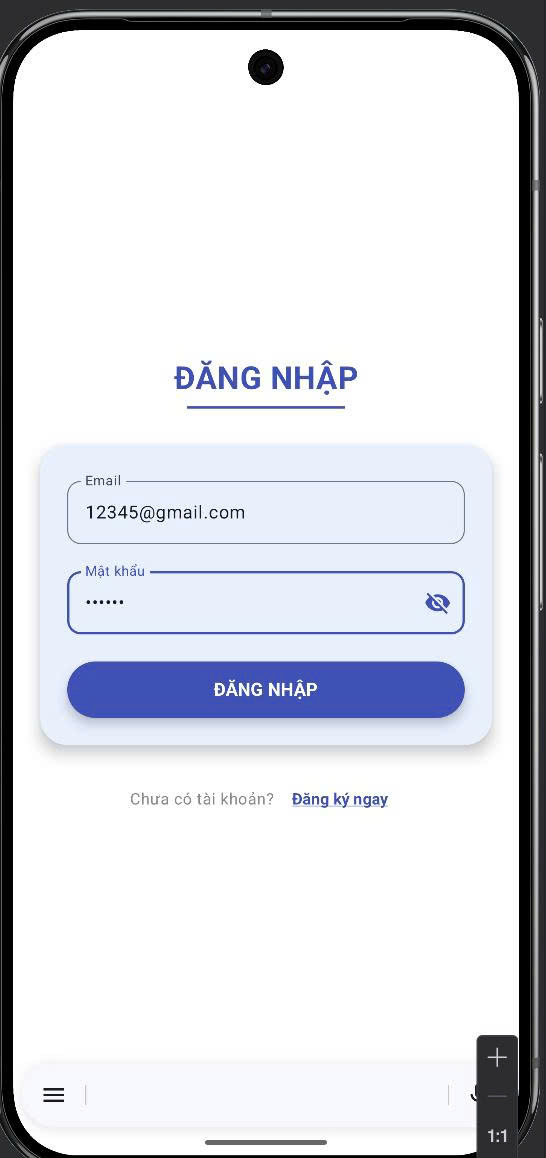
\includegraphics[width=0.5\textwidth]{figures/dang_nhap.jpg}
    \caption{Giao diện mobile app đăng nhập}
    \label{fig:login}
\end{figure}
Hình \ref{fig:login} thể hiện giao diện đăng nhập gồm hai trường Email và Mật khẩu. Người dùng nhấn "ĐĂNG NHẬP" để truy cập hoặc chọn "Đăng ký ngay" để tạo tài khoản mới.
\subsection{Giao diện mobile app người dùng khi chưa đỗ xe}
\begin{figure}[H]
    \centering      
    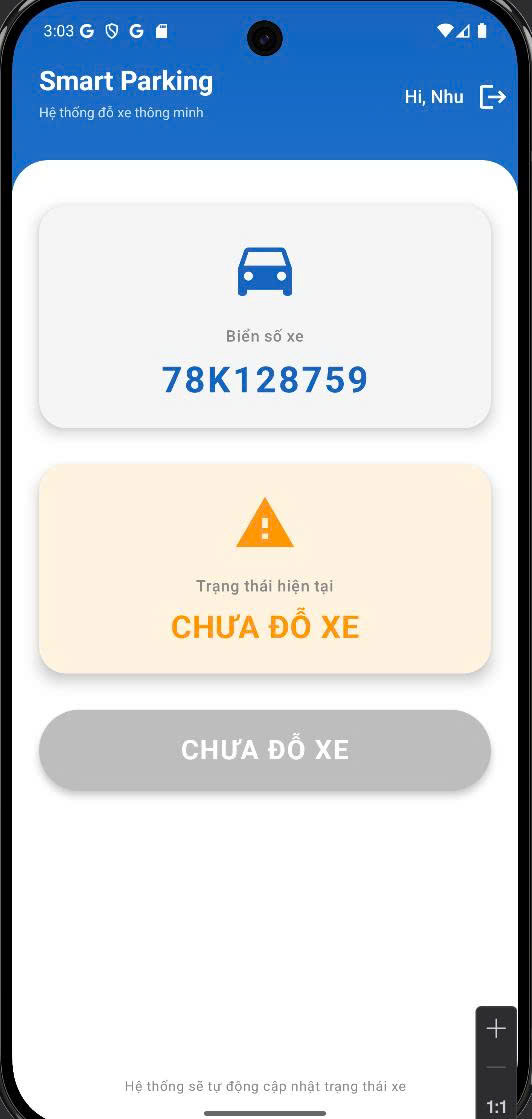
\includegraphics[width=0.5\textwidth]{figures/mah_user_chua_do.jpg}
    \caption{Giao diện mobile app người dùng khi chưa đỗ xe}
    \label{fig:not_parked}
\end{figure}

\subsection{Giao diện mobile app người dùng khi đã đỗ xe}
\begin{figure}[H]
    \centering      
    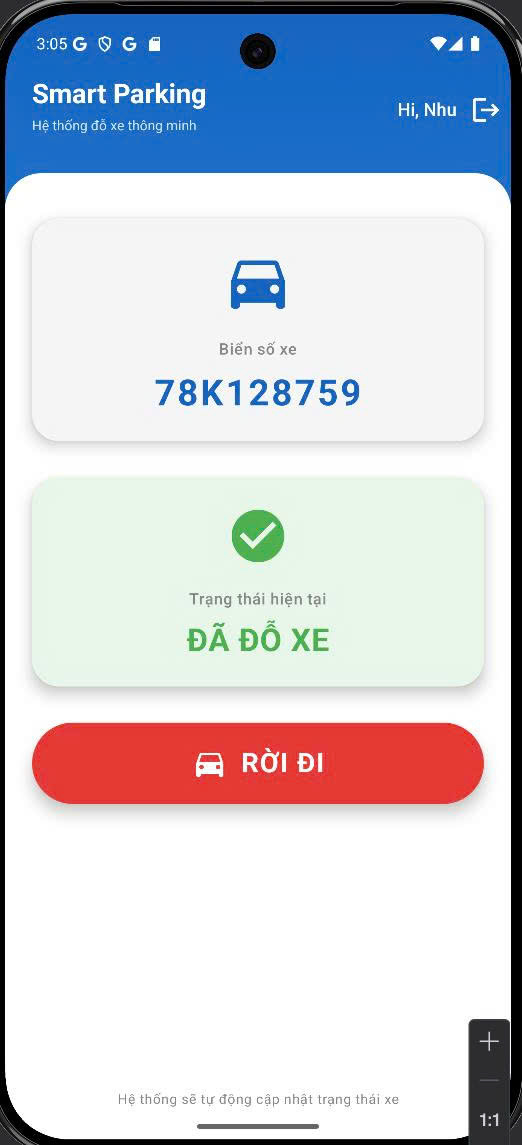
\includegraphics[width=0.5\textwidth]{figures/da_do.jpg}
    \caption{Giao diện mobile app người dùng khi đã đỗ xe}
    \label{fig:architecture}
\end{figure}
\subsection{Giao diện mobile cảnh báo gửi đến người dùng}
\begin{figure}[H]
    \centering      
    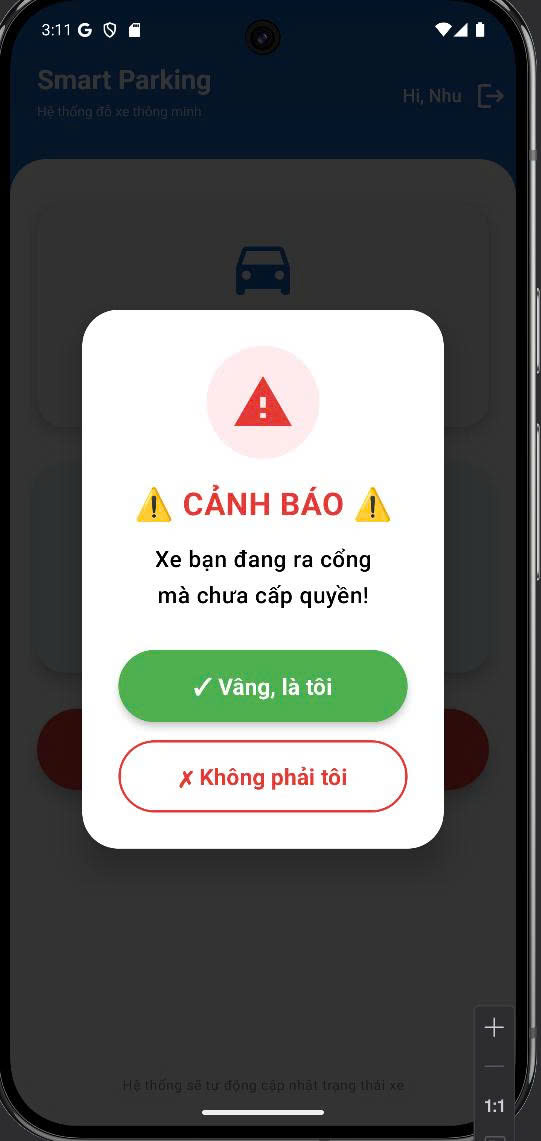
\includegraphics[width=0.5\textwidth]{figures/canh_bao.jpg}
    \caption{Giao diện mobile cảnh báo gửi tới người dùng}
    \label{fig:warning}
\end{figure}
Hình \ref{fig:warning} hiển thị hộp thoại cảnh báo "Xe bạn đang ra cổng mà chưa cấp quyền!" với hai tùy chọn: "Vâng, là tôi" để xác nhận  hoặc "Không phải tôi" để từ chối.
\subsection{Giao diện mobile app bảo vệ}
\begin{figure}[H]
    \centering      
    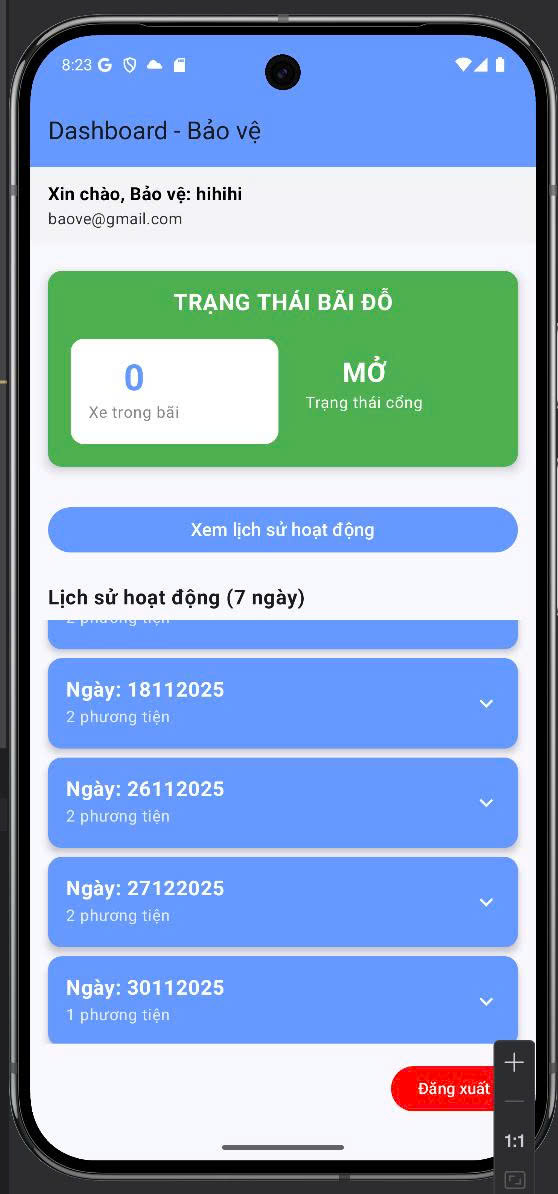
\includegraphics[width=0.5\textwidth]{figures/bao_ve.jpg}
    \caption{Giao diện mobile app bảo vệ}
    \label{fig:dashboard}
\end{figure}
Hình \ref{fig:dashboard} mô tả dashboard của bảo vệ hiển thị trạng thái bãi đỗ (0 xe trong bãi, cổng MỞ) và lịch sử hoạt động 7 ngày gần nhất với số lượng phương tiện ra vào theo từng ngày.


% 13. CHƯƠNG 3

\chapter{CÀI ĐẶT VÀ KIỂM THỬ}

\section{Môi trường và công cụ}


% 14. KẾT LUẬN
\chapter{KẾT LUẬN VÀ HƯỚNG PHÁT TRIỂN}

\section{Kết quả đạt được}

Đề tài đã xây dựng thành công hệ thống quản lý bãi đỗ xe thông minh ứng dụng trí tuệ nhân tạo, đáp ứng các mục tiêu nghiên cứu và yêu cầu thực tiễn đặt ra.

\begin{itemize}
    \item Xây dựng hệ thống nhận diện biển số xe sử dụng YOLO, đạt độ chính xác mAP@50--95 = 91.35\%, đáp ứng yêu cầu bài toán.
    \item Mô hình YOLO nhận diện vùng ký tự trên biển số đạt độ chính xác 66.3\%, cho thấy khả năng phát hiện tốt nhưng vẫn còn hạn chế với các ký tự nhỏ và nhiễu.
    \item Bài toán nhận diện logo xe đạt độ chính xác 35\% (mAP@50--95), phản ánh tính phức tạp cao do kích thước logo nhỏ và sự đa dạng về hình dạng.
    \item Mô hình CNN đọc ký tự đạt độ chính xác 99.7\%, đảm bảo độ tin cậy cao trong giai đoạn nhận dạng ký tự.
    \item Ứng dụng Siamese Network để so sánh và xác thực phương tiện, đạt độ chính xác 100\% trên tập dữ liệu thử nghiệm.
    \item Phát triển hệ thống phần mềm hoàn chỉnh gồm ứng dụng desktop, backend server và mobile app, đáp ứng yêu cầu xử lý real-time.
    \item Tự động hóa quy trình xe vào/ra bãi, giảm thiểu can thiệp thủ công và nâng cao mức độ an toàn, bảo mật hệ thống.
    \item Hệ thống hoạt động ổn định trong điều kiện mạng 4G và WiFi với thời gian phản hồi đáp ứng yêu cầu thực tế.
\end{itemize}




\section{Hướng phát triển}

Trong thời gian tới, hệ thống có thể được tiếp tục phát triển theo các hướng sau:

    \begin{itemize}
        \item Mở rộng và cải thiện dữ liệu huấn luyện nhằm nâng cao độ chính xác nhận diện trong các điều kiện phức tạp.
        \item Tối ưu mô hình và khai thác GPU để cải thiện hiệu năng xử lý thời gian thực.
        \item Tích hợp các chức năng thanh toán tự động và đăng ký phương tiện trực tuyến.
        \item Xây dựng dashboard web cho quản trị viên để quản lý tập trung và theo dõi hệ thống.
        \item Phát triển hệ thống theo kiến trúc linh hoạt, hỗ trợ mở rộng quy mô và quản lý đa bãi đỗ.
    \end{itemize}

Với các kết quả đạt được cùng định hướng phát triển rõ ràng, hệ thống quản lý bãi đỗ xe thông minh có tiềm năng ứng dụng thực tiễn cao, góp phần nâng cao hiệu quả quản lý và cải thiện trải nghiệm người dùng.


% 15. TÀI LIỆU THAM KHẢO
\clearpage
\begin{thebibliography}{99}
\addcontentsline{toc}{chapter}{TÀI LIỆU THAM KHẢO}

\bibitem{siamese_gfg}
GeeksforGeeks, ``Siamese neural network in deep learning,'' \textit{GeeksforGeeks}, 2024. [Online]. Available: https://www.geeksforgeeks.org/nlp/siamese-neural-network-in-deep-learning/. Accessed: Dec. 20, 2024.

\bibitem{yolov8_ultralytics}
Ultralytics, ``YOLOv8 models,'' \textit{Ultralytics Documentation}, 2024. [Online]. Available: https://docs.ultralytics.com/vi/models/yolov8/. Accessed: Dec. 20, 2024.

\bibitem{siamese_hackernoon}
A. Rosebrock, ``One-shot learning with siamese networks in PyTorch,'' \textit{HackerNoon}, 2021. [Online]. Available: https://hackernoon.com/one-shot-learning-with-siamese-networks-in-pytorch-8ddaab10340e. Accessed: Dec. 20, 2024.

\bibitem{cnn_linkedin}
LinkedIn Learning, ``How can you train a convolutional neural network,'' \textit{LinkedIn}, 2023. [Online]. Available: https://www.linkedin.com/advice/3/how-can-you-train-convolutional-neural-network-dtcye. Accessed: Dec. 20, 2024.

\bibitem{deepface_viso}
Viso.ai, ``DeepFace: Face recognition with deep learning,'' \textit{Viso.ai Computer Vision Blog}, 2023. [Online]. Available: https://viso.ai/computer-vision/deepface/. Accessed: Dec. 20, 2024.

\bibitem{jetpack_compose_mvvm}
T. Gis, ``Creating lists in Android Jetpack Compose using MVVM with ViewModel in Kotlin,'' \textit{Medium}, Aug. 2023. [Online]. Available: https://tomasgis.com/creating-lists-in-android-jetpack-compose-using-mvvm-with-viewmodel-in-kotlin-dcfc76945ae7. Accessed: Dec. 20, 2024.

\bibitem{flask_restful_api}
Auth0, ``Developing RESTful APIs with Python and Flask,'' \textit{Auth0 Blog}, 2023. [Online]. Available: https://auth0.com/blog/developing-restful-apis-with-python-and-flask/. Accessed: Dec. 20, 2024.

\end{thebibliography}

\end{document}